\documentclass[
  hyper,    
  lang=cn,
  class=book,
  mathSpec={envStyle=leftbar, alias},
  toc={redef, 2column}
]{zlatex}
\zlatexColorSetup{
  % link        = teal,
  definition  = blue
}
\indexsetup{level=\chapter}
\usepackage{ztikz}
\ztikzLoadModule{cache, wolfram, python, gnuplot, zdraw}
\usepackage{expl3}
\usepackage{xfp}
\usepackage{zhnumber}
\usetikzlibrary{calc}

% optional 
\usepackage{pdfpages}
\usepackage{booktabs}
\usepackage{longtable}
\usepackage{verbatim}
\usepackage{pifont}
\usepackage{multicol}
\usepackage{framed}
\usepackage[bottom]{footmisc}
% TeX logo
\usepackage{xltxtra} 
% minted setup
\usepackage{minted}
\definecolor{bg}{rgb}{0.95,0.95,0.95}
\setminted{
  fontsize=\small,
  bgcolor=bg, 
  breaklines=true, 
  tabsize=2,
  breakanywhere=true,
  breakanywheresymbolpre=,
  breaksymbolleft=,
}
% print macro
\let\cmd\zlatexVerb
\newcommand{\Footnote}[1]{\stepcounter{footnote}\footnote[\thefootnote]{#1}}
\zlatexFramed{leftbar}[gray]
\newcommand{\zkey}[1]{\texttt{<#1>}}
\def\mstyle#1{\noindent\lower.25ex\hbox{\ding{224}}\;\textbf{#1}\par}

% index make
\makeindex[title=部分命令/名词索引, columns=2]


\title{zTikZ manual}
\author{Eureka}
\date{\today}
\begin{document}
\maketitle
\frontmatter
\tableofcontents
\mainmatter
\part{Document}
\chapter{z\LaTeX{}文档类}\label{start-use-class}
\section{基本介绍}
z\LaTeX{}文档类默认基于article文档类,但是你仍然可以在加载本文档类时选择加载其他的文档类,通过设置选项\zkey{class}的值为 
article 或者是 ctexbook 即可. 通过更换默认的文档类,从而满足使用者的不同需求,目前本模板可以用于以下场景:
\begin{itemize}
  \item 撰写书籍或者笔记
  \item 讨论班的Slide制作(可以和article无缝切换)
\end{itemize}

z\LaTeX{}的制作初衷便是:让使用者可以方便进行书籍和笔记的撰写以及日常汇报slide的无缝切换.z\LaTeX{}全部由\LaTeX3进行编写,
采用\cmd{key-value}的方式进行选项配置,对于作者来说:方便后续的模板拓展和维护;对于用户来说:使用键值对可以减轻用户记忆命令参数这一负担,
方便用户使用命令. 如果使用者熟悉\LaTeX{},那么花费不到10min的时间,你便可以轻松使用本文档类完成如上任务,减少不必要的工作.

\section{Set Up z\LaTeX{}}
\subsection{兼容情况}
目前本文档类 z\LaTeX{} 还没有登陆CTAN,未来可能也没有这个打算,本模板还没有完全开发完成.由于本文档类使用的部分
\LaTeX3 命令在老版本下并不存在,所以如果你的 \TeX{}Live 过于老旧,则可能出现无法编译的情况.目前已知
z\LaTeX{}文档类在各平台的兼容情况为:

\hspace*{10em}\parbox{8cm}{
\begin{itemize}
  \item[Windows]: \TeX{}Live最低版本2022
  \item[Linux]: \TeX{}Live最低版本2022
  \item[MacOS]: 兼容Mac{}\TeX{}2024(老版也应兼容) 
\end{itemize}}

\subsection{加载z\LaTeX{}}
由于z\LaTeX{}还没有传入CTAN(未来可能会考虑),所以想要使用此文档类,可以有如下的两种方法:
\begin{itemize}
    \item 把此文档类-\cmd{zlatex.cls}放入当前项目文件夹下
    \item 在命令行运行命令: \cmd{kpsewhich -var-value=TEXMFHOME}, 然后把\cmd{zlatex.cls}放入此路径下的
        \cmd{tex/latex/}子目录下. 在Windows上一般是: \cmd{C:/Users/<name>/texmf/}, 在Linux下一般是
        \cmd{~/texmf/},具体路径以自己的实际情况为准.
\end{itemize}

\subsection{额外设置}
z\LaTeX{}默认只加载部分的基础宏包,所以想要实现其它的功能还请自行引入相关的宏包;
z\LaTeX{}引入的宏包机制请参见\cref{tab:basic-package}.在默认情况下本模板即可呈现一个比较好的
效果,所以不熟悉\LaTeX{}的用户不用担心本模板配置选项过于复杂. 想要马上开始体验? 请参
见``\cref{最小工作示例}''的最小写作示例.

\subsection{最小工作示例}\label{最小工作示例}
z\LaTeX{}的最小工作示例如下\Footnote{导言区的配置可能需要根据自己的实际情况加以调整,详细配置请参见后文}.
首先是中文写作示例,默认加载 {article} 文档类,如果喜欢使用 {book} 文档类,可以在加载文档类时
指定\cmd{class=book}.

\begin{minted}{latex}
% compile engine: xelatex 
\documentclass[lang=cn]{zlatex}

\begin{document}
% some preface
% \tableofcontents

% wrting your document here ...
\end{document}
\end{minted}

其次是英文写作示例(此时为{book}文档类),你需要修改的地方只有两处;首先就是把语言选项改为\cmd{lang=en},
其次便是把编译方式改为{pdflatex}.

\begin{minted}{latex}
% compile engine: pdflatex 
\documentclass[class=book]{zlatex}

\title{<title>}
\author{<author>}
\date{<date>}
\begin{document}
\maketitle
\frontmatter
% some preface
% \tableofcontents
% some claim etc.
\mainmatter

% wrting your document here ...
\end{document}
\end{minted}

\subsection{在线体验}
为了让部分用户可以直接体验到 z\LaTeX{},免去``繁杂''的环境配置.我已将本模板部署在 Overleaf 上,
地址为:\href{https://www.overleaf.com/project/661fd2772cafbff9df5e6fb4}{Overleaf ZLaTeX Project},
直接打开此地址即可体验.Overleaf上的项目内容为本手册的源码,不含有 zTikZ 文档. 由于部分的技术原因,zTikZ 
请在本地体验.

\section{宏包机制}
z\LaTeX{}文档类会根据用户指定的选项自动处理和加载对应的宏包,所以z\LaTeX{}文档类在不同的导言区选项声明下
加载的宏包和命令是不同的.本文档类内置导言区选项输出命令:\cmd{\zlatexOptions}\index{\cmd{\zlatexOptions}},
用于打印此时文档类z\LaTeX{}接收到的选项. 比如此时文档类接收到的选项为: 
\begin{center}
    \zlatexOptions
\end{center}

以下为详细的宏包加载信息:

\subsection{基本宏包}
基本宏包\index{basic packages},意味着不管你的导言区如何的配置,这些宏包都是会加载的. 宏包列表如下:

\begin{table}[H]
    \centering{
    \begin{tabular}{p{3cm}p{3cm}p{3cm}p{3cm}}
        \toprule
        expl3 & l3keys2e & framed & geometry \\
        fancyhdr & amsfonts & amsmath & amsthm  \\
        xcolor & biblatex & indextools & sidenotes \\ 
        cleveref & graphicx & float & titletoc \\
        titlesec & esint &  \\
        \bottomrule
    \end{tabular}}
    \caption{z\LaTeX{}文档类基本宏包}
    \label{tab:basic-package}
\end{table}

\subsection{语言类宏包}
根据不同的文档类语言,z\LaTeX{}会加载不同的和语言相关的宏包\index{language packages},在\cmd{lang=en(cn)}
下的宏包加载列表分别为:

\begin{table}[H]
    \centering{
    \begin{tabular}{p{2cm}p{4cm}p{2cm}p{2cm}p{2cm}}
        \toprule
        {\rmfamily lang=en} & inputenc(pdftex) & fontenc \\
        {\rmfamily lang=cn} & fontspec & ctex \\
        \bottomrule
    \end{tabular}}
    \caption{z\LaTeX{}文档类语言宏包}
    \label{tab:lang-package}
\end{table}

在\LaTeX{}排版中,正确使用{\bf 引号}的方法是分别使用\cmd{`}和\cmd{'}排版单引号`和',
分别用\cmd{``}和\cmd{''}排版双引号``和''.\cmd{``}和\cmd{`}会被转换成opening quotation marks,后两者会被转化成
closing quotation marks.另外,在排版要求中,当两层双引号嵌套使用时,其外层需要使用{\bf 双引号},而内层则应该使用{\bf 单引号},
并且不同的语言中,用于表示引号的字符也不完全一致.为解决这些排版中的问题,可以使用 {csquotes} 宏包实现引号的灵活排版
\Footnote{本内容摘自\href{https://wenda.latexstudio.net/article-5042.html}{latexstudio}},比如要使用双引号文本,那么此时
你就可以使用命令\cmd{\enquote{<your text>}}.

\begin{leftbar}
  但是你也可以直接在源文件中输入对应的unicode,如果你使用的是Xe\TeX{}或者是加载了inputenc的utf8选项.
\end{leftbar}

\subsection{数学字体类宏包}
本模板会根据导言区选项加载不同的数学字体. 为方便新手较使用不同数学字体,本模板预设了几个简单的数学字体.
用户只需配置导言区即可实现不同数学字体的加载. 具体的宏包\index{math packages}加载规则如下:
\begin{itemize}
    \item \cmd[F]{mathSpec={font=<none>}}: 不加载任何的数学字体宏包,采用默认数学字体
    \item \cmd[F]{mathSpec={font=newtx}}: 加载宏包 {newtxmath}
    \item \cmd[F]{mathSpec={font=euler}}: 加载命令 \cmd[F]{\RequirePackage[OT1, euler-digits]{eulervm}}
    \item \cmd[F]{mathSpec={font=mtpro2}}: 加载命令 \par
        \cmd[F]{\RequirePackage[lite,subscriptcorrection,slantedGreek,nofontinfo]{mtpro2}}
    \item \cmd{font=mathpazo}: 加载命令 \cmd[F]{\RequirePackage{mathpazo}},同时保留了文档类默认的正文字体样式.
\end{itemize}

如果使用者在导言区还指定了选项\cmd{mathSpec={alias=true}}, 那么z\LaTeX{}此时还会额外加载
的宏包\index{optional packages}:{amssymb, mathtools, bm}.

除此之外, z\LaTeX{} 还默认加载了宏包{esint}, 用于提供部分积分符号变体.下面仅举几例,更多的人信息请参见{esint}宏包文档:
\[
  \iiint\qquad 
  \idotsint\qquad
  \ointclockwise\qquad
  \fint\qquad
  \landdownint
\]

其实还有一个包和 {esint} 类似,叫做 {pdfMsym}. 关于后者的使用请参见 pdfMsym 官方文档:\href{https://mirror-hk.koddos.net/CTAN/macros/generic/pdfmsym/pdfmsym-doc.pdf}{pdfMsym}.

\begin{leftbar}
如果用户想自己设置文档的数学字体,那么请参见"字体配置\cref{font-config}"中的数学字体配置部分.
\end{leftbar}

\subsection{超链接宏包}
z\LaTeX{}文档类现在不默认加载宏包 hyperref, 但是在加载文档类时指定\cmd{hyper=true}即可加载此宏包以及对应的配置.其实还是考虑
到编译速度的问题,一般在初稿阶段:作者是不需要这部分超链接功能的,此宏包引入后需要的多次编译也十分不必要,所以我便把 hyperref
从基本宏包中移除.

\section{文档类选项与命令}
本模板具有丰富的配置选项\index{配置选项}, 采用键值对\cmd{[<key 1>=<value 1>, <key 2>=<value 2>]}的形式对各个选项就行指定, 和具体的指定顺序无关, 
具体的可配置项和可用的配置值参见本节的后续内容以及\cref{fig:zlatex-options}. 现在先简要说明z\LaTeX{}文档类的主要配置内容:

\begin{itemize}
    \item 模板语言\index{模板语言}:目前本模板类仅支持中文和英文两种语言.
    \item 文档类选择\index{文档类选择}:可以在加载本文档类时指定 {article, book, ctexbook}.
    \item 展示方式\index{slide mode}: 默认情况下以普通的文档展示,也可以指定\cmd{layout={slide}}
      选项后把文档转化为 beamer,详细使用请参见:\cref{sec:slide-mode}.
    \item 页面设置\index{页面设置}:页边距,版心,页眉页脚等的指定;目前本模板还未整理好对应的接口,但用户可以通过
      geometry/fancyhdr 宏包提供的接口进行设置.
    \item 边注\index{边注}(marging):包含编注图片或文字注释,其中边注图片依赖宏包\cmd{sidenotes}.
    \item 数学字体\index{数学字体}:本模板预设了5种数学字体配置.
    \item 字体配置\index{字体配置}:用户可根据自己喜好配置相应的中英文字体,具体配置方法参见:\cref{font-config}.
\end{itemize} 


\subsection{导言区}
目前 z\LaTeX{} 的配置选项可以在文档类加载时指定,也可以通过命令 \cmd{\zlatexSetup}进行指定.键值对被划分为两个层级:第一级
中主要的键为:\zkey{layout, mathSpec, font, bib, classOption, lang, toc}. 其中前四个键(key)具有自己的独立的子键(sub-key),
后两者不具有自己的子键,直接指定即可. 关于各层 key-value 的关系请见\cref{fig:zlatex-options}.

\begin{figure}[!htb]
    \centering
    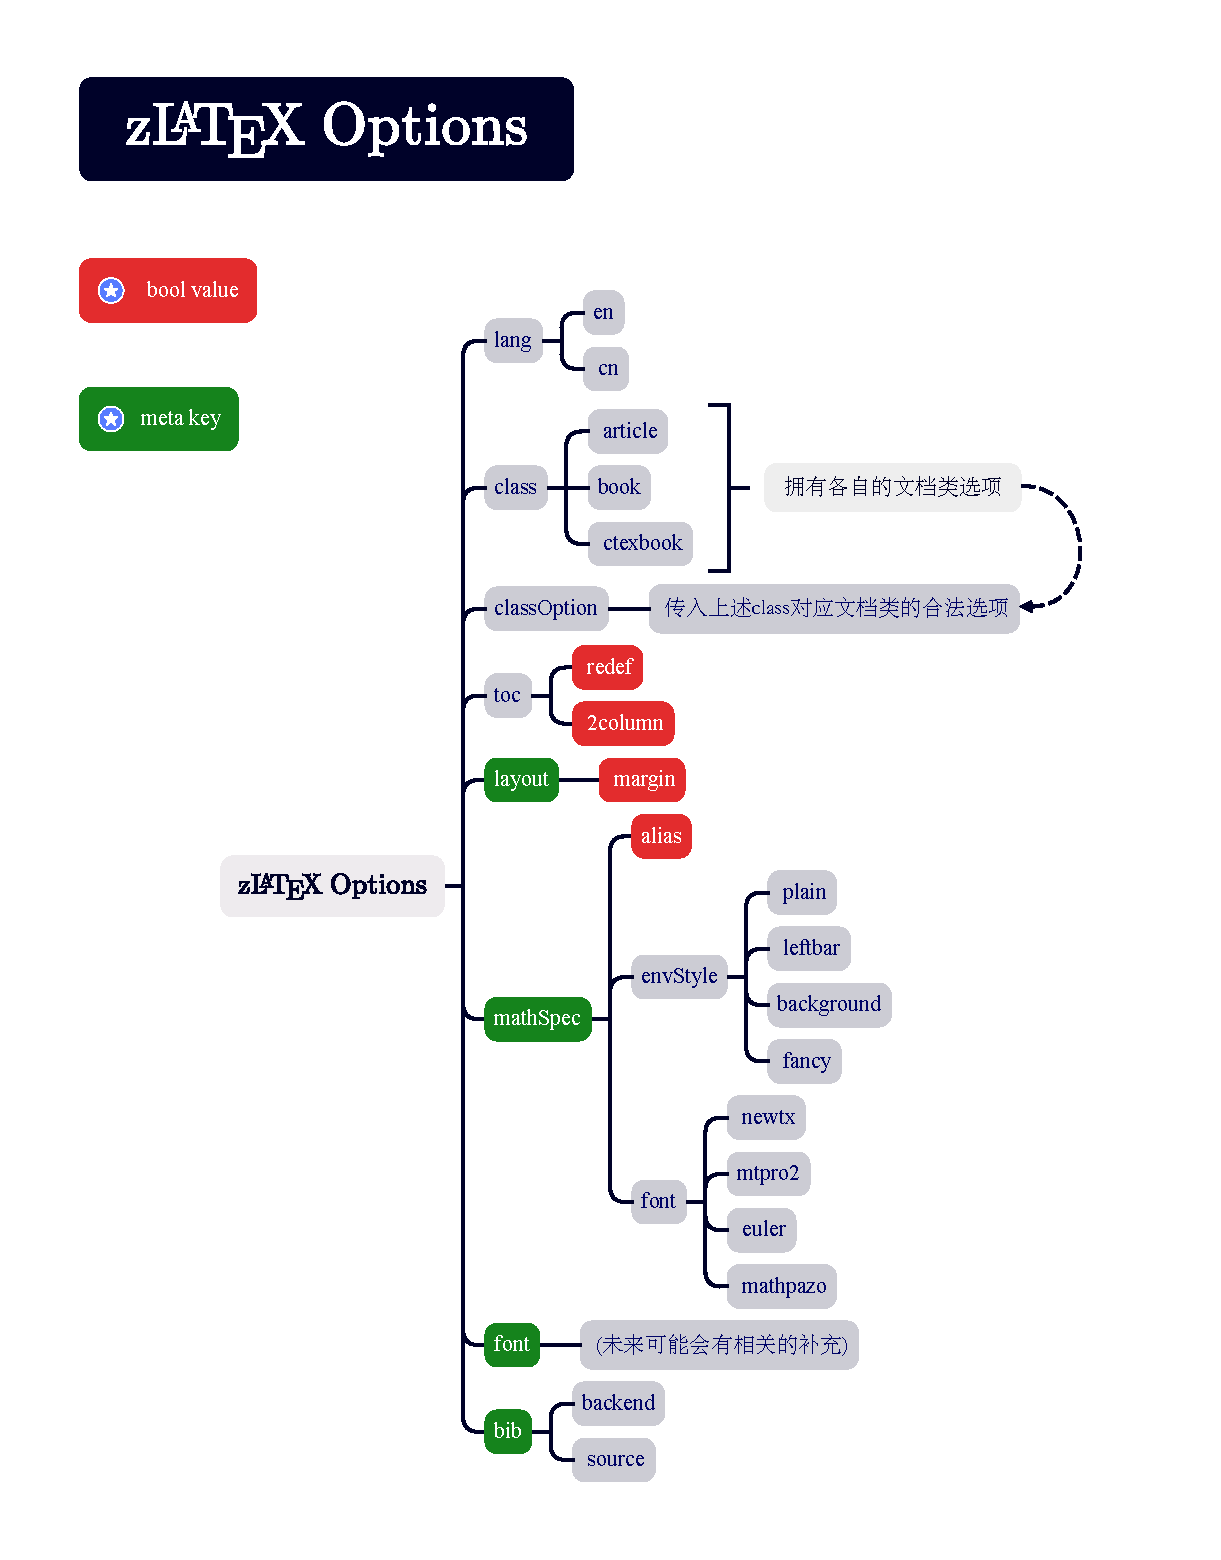
\includegraphics[width=.9\linewidth]{./pics/zlatex_options.pdf}
    \caption{zlatex options map}
    \label{fig:zlatex-options}
\end{figure}

从\cref{fig:zlatex-options}可以看出,z\LaTeX{} 的配置是比较复杂的,但是刚接触本文档类时,用户也不必担心,默认的选项配置下
已经能够得到一个效果比较好的文档了.下面详细说明各个键的指定方式和作用. 

\mstyle{classOption}
这里的\zkey{classOption}表示你加载的对应文档类的合法 options. 比如 {article} 文档类,合法的一个设置为:\cmd{classOption
={10pt, oneside, fleqn}}. 如果你在加载文档类时指定的\zkey{class}为 {ctexbook},那么此时你可以在\zkey{classOption}
中填入如下像:\cmd{zihao=5, 12pt, heading=false, linespread=1.3} 等 {ctex} 手册中说明的合法选项. 若对于默认的 article,
book 文档类不熟悉,可以参见:\href{https://texblog.org/2013/02/13/latex-documentclass-options-illustrated/}{latex-documentclass-options}.

\mstyle{lang}
键\zkey{lang}的合法值为 {en, cn}; 第二个关于文档语言的指定是比较容易理解的,但是还是得说明对应的一些注意事项.\cmd{lang=cn}或者\cmd{class=ctexbook}时
仅支持为\hologo{XeLaTeX}编译;在指定\cmd{lang=en}时, \hologo{pdfLaTeX}, \hologo{XeLaTeX} 二者都是可以接受的,但是建议使用 \hologo{pdfLaTeX}. 因为在指定\cmd{lang=en}时部分的西文宏包
可能会有冲突的危险.当指定\cmd{lang=en}, 并且采用 \hologo{pdfLaTeX} 进行编译时,z\LaTeX{}会引入宏包 {inputenc}, 然而此宏包对 \hologo{XeLaTeX} 是
没有适配的.

\mstyle{toc}
键\zkey{toc}的合法值为\cmd{redef, 2column},这一选项主要用于文档的目录格式设置,可以设置目录页对应的标题,目录的栏数.
\zkey{toc}\index{\cmd{toc}}选项可以同时指定\cmd{redef, 2column},分别代表重定义目录名(居中加粗),以及排版双栏目录.
后续可能会把这个键\zkey{toc}放入\zkey{layout}中.所以目前此接口还不稳定, 请谨慎使用.

\mstyle{bib}
本模板的默认参考文献后端为 {biber},可以在导言区通过\cmd{backend=bibtex}来更改默认后端为\cmd{bibtex}.这说明,在默认配置下,
你编译文档时应在命令行使用 {biber} 命令, 而非 {bibtex} 命令. 同样的,可以通过\zkey{bib}的子键\zkey{source}来指定参考文献对应的文件名,
默认文件名为: {ref.bib}. 

\mstyle{layout}\label{sec:slide-mode}
\zkey{layout} 键可用于指定整个文档布局:版心,页边距,边注间距等,也可以指定文档最终的呈现方式:普通的文档,还是展示所用的slide.
目前模板提供子键\zkey{margin, slide}用于设置对应布局. 此键合法值为bool值, 指定方式如下:
\begin{minted}{latex}
% {margin} <=> {margin=true}
\documentclass[
    layout={margin, slide}
]{zlatex}
\end{minted}

默认情况下\zkey{margin}的值为\cmd{false}. 如果使用了上述键值指定,那么此时的文档就会产生一个边注. 一般情况下,如果不是撰写相应的书籍,
使用者是不需要加载这个选项的. \textbf{需要注意}:\cmd{margin=false} 只有在\cmd{oneside} 时才有效,否则会抛出警告. 如果原文档中含有\cmd{\marginpar}
命令,那么在指定\cmd{margin=false}后,对应的\cmd{\marginpar}环境,会被替换为\cmd{framed}宏包提供的\cmd{leftbar}环境.

\begin{remark}
默认情况下 \cmd{twoside} 选项对应的 margin 和 \cmd{margin} 选项对于的 margin 宽度是不同的,后者比前者宽一些.
\end{remark}

如果你需要将最终的文档编译为演示文档, 除了必须加载\zkey{slide}选项外,你还可以指定幻灯片比例, 使用\zkey{aspect}子键进行设置,
默认的比例为\cmd{16:9},默认的长度单位为厘米(cm). 如果你想要设置幻灯片的比例为12:9,那么导言区按照如下设置即可:
\begin{minted}{latex}
\documentclass[
  layout={slide, aspect=12|9},
]{zlatex}
\end{minted}

也就是使用符号``|''进行两个维度上距离的分割. 关于slide 模式下的主题:目前还不支持自定义,后续可能会进行拓展. 如果仅仅只是想要修改
slide 中不同元素对应的颜色,那么只需重新定义如下三个颜色:
\begin{itemize}
  \item \cmd{slideRed}: \block{slideRed}
  \item \cmd{slideGray}: \block{slideGray}
  \item \cmd{slideWhite}: \block{slideWhite}
\end{itemize} 

下面为一默认 slide 模式样例:
\begin{figure}[!htb]
  \centering
  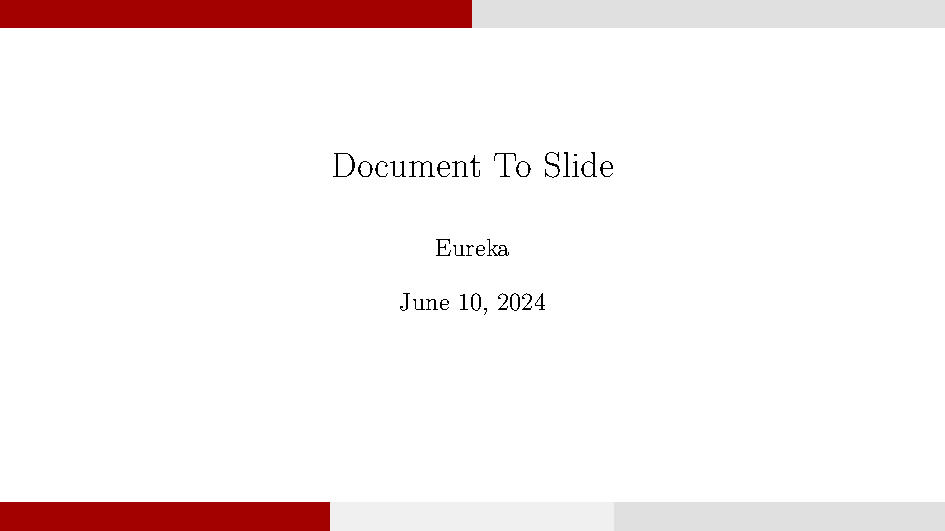
\includegraphics[width=.45\linewidth]{./pics/doc2slide_1.pdf}
  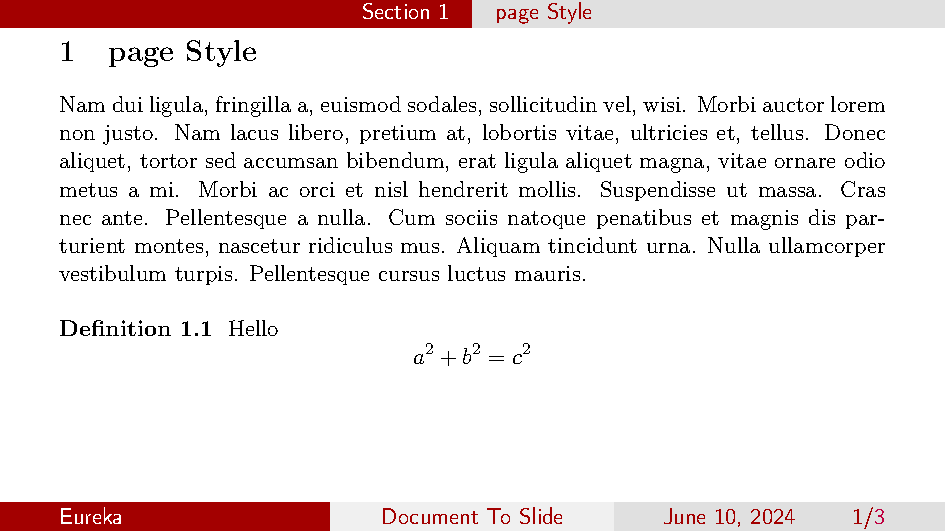
\includegraphics[width=.45\linewidth]{./pics/doc2slide_2.pdf}
  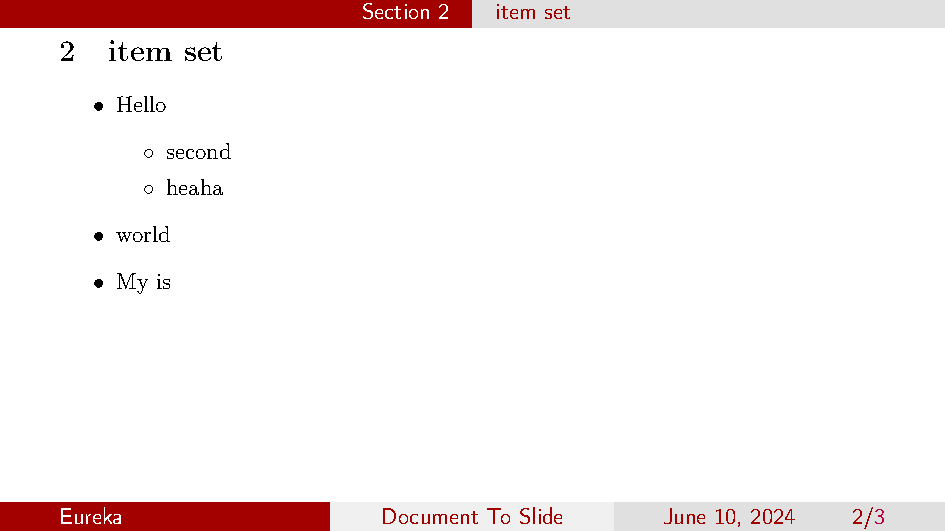
\includegraphics[width=.45\linewidth]{./pics/doc2slide_3.pdf}
  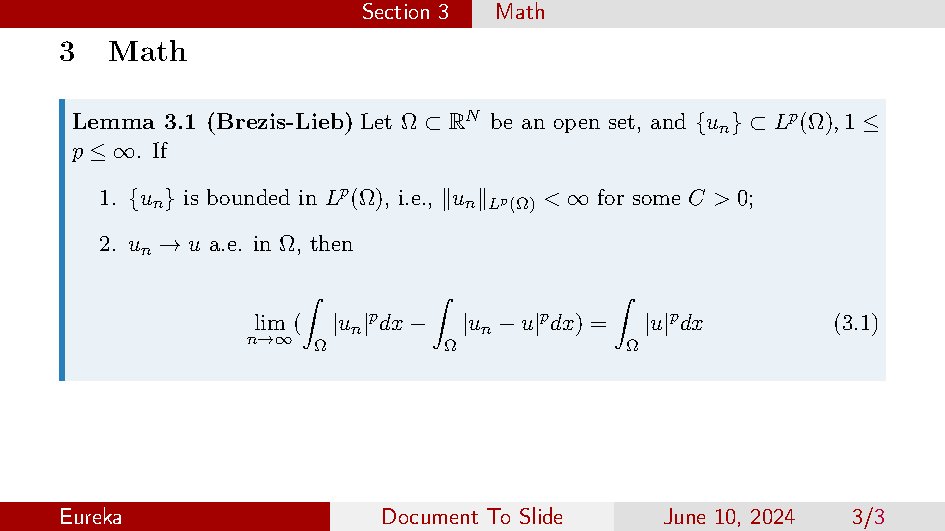
\includegraphics[width=.45\linewidth]{./pics/doc2slide_4.pdf}
  \caption{Slide 样例}
  \label{fig:slide-example}
\end{figure}

\begin{leftbar}
目前 slide 模式还处于一个很不成熟的阶段,请谨慎使用. 在正式场合请使用默认的 beamer 文档类.
\end{leftbar}

\begin{remark}
由于本模板可以切换单双面布局,所以为了保证 titlepage 中文字的正确居中,本文档类对原始命令:\cmd{\maketitle} 进行了重定义.
除了本文档类定义的 \cmd{\maketitle} 命令外,本文档类还提供了命令 \cmd{\Maketitle} 用于排印简洁的封面页,效果相当于原始{\bfseries 命令+居中}.
本模板保留原始命令为 \cmd{\orimaketitle}, 那么这三个命令到底该怎么用?  下面给出一个情况下的应用规则:
\begin{itemize}
  \item 在 slide mode 下使用 \cmd{\orimaketitle} 命令
  \item 在 oneside 布局下使用 \cmd{\maketitle, \maketitle} 均可
  \item 在 twoside 布局下使用 \cmd{\Maketitle} 命令排印原始封面页+居中+换页,\cmd{\maketitle}命令排印自定义的封面页+换页
\end{itemize}
\end{remark}

\mstyle{mathSpec}
此选项可用于设置文档类对应的数学字体等内容, 本文档类预设了几种数学字体和定理环境样式以及部分数学命令别称. 详细信息如下:
\begin{itemize}
    \item 数学字体(\cmd{font=name}):可用\cmd{name}:\cmd{newtx, mtpro2, euler, mathpazo}
    \item 定理类环境样式(\cmd{envStyle=name}):可用\cmd{name}:\cmd{plain, leftbar, background, fancy}
    \item 字体命令 alias 加载(\zkey{alias}):可以直接输入\cmd{alias, alias=false}或者是输入\cmd{alias=true, alias=false}
\end{itemize}

一个简单的例子:如果你想设置键(\zkey{mathSpec})对应子键:\cmd{font, envStyle, alias}的值(value), 其中最后一个 key 为 bool 值.
那么你可以在导言区中这样设置:

\begin{minted}{latex}
\documentclass[
    mathSpec={
        alias,
        envStyle=background,  
        font=newtx
    },
]{zlatex}
\end{minted}

上述的声明表示,文档类的定理类数学环境样式为:\cmd{background},数学字体为\cmd{newtxmath}. 同时加载了数学命令别名.
其实所谓的命令别名就是如下常用命令的缩写:
\begin{minted}{latex}
\mathbb{X}    \mathcal{X}    \mathrm{X}   ...
\end{minted}

可以替换为如下更加简洁的形式:
\begin{minted}{latex}
\B{X}    \C{X}    \R{X}    ...
\end{minted}

对于\LaTeX{}, 新手千万不要秉持着:``少些就是赚到'' 的观念,你保持不住. 但是你完全可以定义空格为你的 delimiter,以此来划分你的宏参数. 
所以你可以写这种东西:
\begin{minted}{latex}
% define macro
\def\upb#1 #2 {\mathbb{#1}^{#2}}
% use macro
\upb R N^2 = \upb R N \times \upb R N \cdots
\end{minted}

这个结果和你添加括号无异, 但是一旦你落下了某个重要的空格,那么轻则编译结果不正确,重则编译不通过.

关于 \cmd{alias} 配置的详细声明细节,请参见章节"快捷命令\cref{快捷命令}". \cmd{alias} 选项可根据个人习惯进行选择加载,默认
情况下并不会加载.但在加载此选项后,默认的两个\LaTeX{} 宏 \cmd{\S, \ll} 会被重定义,分别被更名为 \cmd{\ss, \LL}:(\ss, $\LL$). 

需要注意:本模板提供的部分数学字体并不一定符合每人审美,且由于本模板在 Linux 环境下开发,所以在平台迁移后部分字体可能会有细微的差别.
其中的 {mtpro2} 字体并非免费字体, 请不要用于任何的商业用途. 若用户想自己配置数学字体,那么可以参见后文``Unicode-math:\cref{数学字体}''

\begin{leftbar}
关于\cmd{envStyle}的详细信息请参见:"常用数学环境\cref{常用数学环境}"
\end{leftbar}

\subsection{快捷命令}\label{快捷命令}
在你决定加载选项\cmd{alias}\index{\cmd{alias}}前的进一步说明:默认自定义命令并不一定符合你的习惯,所以请一定谨慎加载此选项.
在\cmd{alias=true}后,z\LaTeX{}会进行如下命令的声明/重定义,以及部分宏包的加载:
\begin{minted}{latex}
\RequirePackage{amssymb, mathtools}
\RequirePackage{bm}          
% Math Font 
\newcommand{\dd}{\mathrm{d}}
\newcommand{\C}[1]{\ensuremath{\mathcal{#1}}}
\let\ss\S
\renewcommand{\S}[1]{\ensuremath{\mathscr{#1}}}
\newcommand{\B}[1]{\ensuremath{\mathbb{#1}}}
\newcommand{\FF}[1]{\ensuremath{\mathbf{#1}}}
\newcommand{\F}[1]{\ensuremath{\bm{#1}}}
\newcommand{\R}[1]{\ensuremath{\mathrm{#1}}}
\newcommand{\K}[1]{\ensuremath{\mathfrak{#1}}}
% Math Arrow 
\newcommand{\lr}{\ensuremath{\longrightarrow}}
\let\LL\ll
\renewcommand{\ll}{\ensuremath{\longleftarrow}}
\newcommand{\equ}{\ensuremath{\Longleftrightarrow}\,}
\newcommand{\sr}{\ensuremath{\longmapsto}}
\newcommand{\lrr}[2][]{\ensuremath{\xRightarrow[#1]{#2}}}
\renewcommand{\lll}[2][]{\ensuremath{\xLeftarrow[#1]{#2}}}
\newcommand{\ns}{\ensuremath{\varnothing}}
\newcommand{\A}{\ensuremath{\forall}}
% Math Operator
\newcommand{\alt}{\ensuremath{\mathrm{Alt}\;}}
\newcommand{\sgn}{\ensuremath{\mathrm{sgn}\;}}
\newcommand{\curl}{\ensuremath{\mathrm{curl}\;}}
\newcommand{\grad}{\ensuremath{\mathrm{grad}\;}}
\newcommand{\trace}{\ensuremath{\mathrm{trace}\;}}
\renewcommand{\div}{\ensuremath{\mathrm{div}\;}}
\end{minted}

若用户认为上述的某些数学运算符声明并不是那么规范,如果有必要,可以自行进行修改,可参见
命令\cmd{\DeclareMathOperator}, \cmd{\DeclareMathAlphabet}.

\subsection{zlatexSetup}
本模板同样也提供了命令\cmd{\zlatexSetup}用于在导言区对整个文档进行设置,其使用方法和前面的几乎是一致的. 如下
两段声明等价:
\begin{minted}{latex}
\documentclass[
    mathSpec={envStyle=background, alias, font=mathpazo},
    toc={redef, 2column},
    bib={backend=bibtex}
]{zlatex}
\end{minted}

\begin{minted}{latex}
\zlatexSetup{
    mathSpec={
        envStyle=background,
        font=mathpazo, 
        alias
    },
    toc={redef, 2column},
    bib={backend=bibtex}
}
\end{minted}

但是命令\cmd{\zlatexSetup}并不能对所有键进行指定,如\zkey{class}, \zkey{lang} 这两者只能在加载文档类时声明, 不能在后续
使用此命令声明. 同时,本命令不包含本文档类的颜色主题设置,和颜色主题设置相关类容请参见命令:\cmd{\zlatexColorSetup},关于
本文档类的默认色彩设置请参见``模板配色\cref{模板配色}''. 

如果你加载了宏包 {ctex},那么此时你也可以使用此宏包提供的命令\cmd{\ctexset}进行对应元素的设置.

\subsection{zlatexColorSetup}\label{模板配色}
z\LaTeX{}提供了命令\cmd{\zlatexColorSetup}\index{\cmd{\zlatexColorSetup}}用于整个模板的配色设置,
可供用户配置的选项:
\begin{itemize}
    \item hyperref 宏包对应的颜色,对应的键:\zkey{link, url, cite}, 三者颜色默认不同.
    \item chapter 章节计数器颜色,对应的键:\zkey{chapter}.
    \item chapter 章节 chapter ruler 的前景色,对应键:\zkey{chapter-rule}.
    \item 所有数学环境对应的颜色,对应的键:\zkey{math-env-name}, 如\zkey{axiom, definition, theorem, remark}等.
\end{itemize}

下面给出一个设置文档类配色的示例代码:
\begin{minted}{latex}
\zlatexColorSetup{
    link            = purple,
    chapter-rule    = black,
    axiom           = purple,
    definition      = blue
}
\end{minted}

本文档类的默认配色如下:
\begin{table}[H]
    \centering
    \begin{tabular}{ccccccccc}
        \toprule
        结构元素 & chapter & chapter-rule & link & url & cite \\
        \midrule 
        颜色 & \block{RoyalRed} & \block{black} & \block{purple}& \block{RoyalRed} & \block{blue}\\
        \midrule
        数学环境 & axiom & definition & theorem & lemma & corollary & proposition & remark & \\  
        \midrule 
        颜色 & \block{mathaxiomColor} & \block{mathdefinitionColor} & \block{maththeoremColor} & \block{mathlemmaColor}& \block{mathcorollaryColor}& \block{mathpropositionColor}& \block{mathremarkColor}\\
        \bottomrule
    \end{tabular}
    \caption{z\LaTeX{}文档类默认配色}
    \label{tab:zlatex-default-color}
\end{table}


\subsection{zlatexFramed}
目前本模板还提供了命令\cmd{\zlatexFramed{<name>}[<color>]}\index{\cmd{\zlatexFramed}}用于创建类似 MarkDown
的引用环境. 参数中\zkey{name}表示声明环境名称\footnote{如果此环境已存在,那么该环境会被 Override},
\zkey{color} 表示此环境的背景颜色.一个简单的使用样例如下:

\begin{minted}{latex}
% 环境 'refer' 声明
\zlatexFramed{refer}[orange]
% 使用环境 'refer'
\begin{refer}%
% something wrting here
\end{refer}
\end{minted}

\zlatexFramed{refer}[orange]
\begin{refer}%
As any dedicated reader can clearly see, the Ideal of practical
reason is a representation of, as far as I know, the things in themselves;

劳仑衣普桑,认至将指点效则机,最你更枝.想极整月正进好志次回总般,段然取向
使张规军证回,世市总李率英茄持伴.
\end{refer}

\begin{leftbar}
  在上面的refer环境开始时插入一个\%可以用于消除多余空格
\end{leftbar}

\section{z\LaTeX{}接口}
z\LaTeX{} 的接口正在不断的完善中,所以目前的接口可能并不是那么稳定(我已然尽力). 

\subsection{命令声明}
后续可能会考虑声明一个用于定义键值对命令的接口,而不是默认的位置参数或者是 xparse 提供的可选参数等.
依托于 \LaTeX3 的 {key-value}模块,这样的接口会更加的灵活,更加的方便用户使用.


\subsection{盒子接口}
通过\LaTeX3 的盒子接口进行接口的定制可能并不是后续的一个模板开发重点. 如果要开发,也是主要基于宏包 {xcoffins} 已提供命令的再次封装, 在万不得已时
我不会做这部分的底层工作. 一般情况下有了 {xcoffins} 宏包后便可以进行大部分的操作了,如果使用者还需要绘制部分复杂的图形只能够借用 {tikz}
宏包,不妨先在另一个文档类中生成对应的 pdf 文件,然后在正文中直接插入 pdf 即可. 目前 xcoffins 宏包的接口已经稳定,详细信息请参见
\begin{itemize}
    \item \href{https://ctan.org/pkg/l3experimental}{l3experimental}
    \item \href{https://tex.stackexchange.com/a/397835/294585}{interface of xcoffins}
\end{itemize}

一般盒子操作对于 \LaTeX{} 的普通使用者来说可能难度比较大,所以要提供一个便于用户使用,同时还要保证接口的统一性的系列命令是不容易
的,所以 z\LaTeX{} 盒子接口还没有开始编写. 其实如果用户能够完成盒子的声明,盒子(join box)简单拼接等操作,那么这就已经足够了.
更进一步,若用户能够对盒子进行一些常规的操作:包括盒子的 resize, scale, rotate. 那么大部分的复杂操作你都能够自己实现了 (除去少部分
必须使用tikz).


\subsection{绘图接口}
本文档类在将来并不打算引入 {tikz} 宏包,一方面个人觉得 tikz 宏包过于庞大, 很多功能并不都是一个文档类所应必须拥有的.
也许会在后续引入 {l3draw}\index{\cmd{l3draw}} 模块用于替代部分的 tikz 命令. 

因为本文档类可能会抛弃 {tikz, tcolorbox} 等宏包,所以在后续版本中可能需要加入 \cmd{xcoffins, l3draw, l3opacity}
等隶属于 l3experimental 的宏包. 基于这些宏包定制属于 z\LaTeX{} 的接口,从而提供对应的用户接口, 完善图形绘制功能等.
这些宏包大部分还处于 experiment 阶段,自然 z\LaTeX{} 的这部分接口自然也可能会在不久的将来改变, 请见谅. 同样的,
\cmd{l3draw} 其实还不能完全实现 PGF 的功能,如 shade 操作.

\begin{leftbar}
本文档类配套的 {zTikZ} 模块(宏包)提供了丰富功能:如 TikZ绘图,数值计算,符号计算以及部分的图像处理功能. 具体使用请参见
ztikz\_manual.pdf.
\end{leftbar}

\subsection{算法与数据结构}
在 \LaTeX{}3 中其实已经提供了很多的常用数据结构:列表(token list, sequence, clsit), 字典(prop list), 整形数组(int array), 
浮点数组(fp array). 其实其中也提供了基本的堆,栈,队列等常用数据结构.使用已有的这些元素来构造如: 图, 树等结构也不是特别困难的.

在\LaTeX3中实现常用的算法可以么? 当然可以,而且有了 \LaTeX3 的宏展开机制,相较于在原本的 \LaTeX 2e 中实现,在现阶段要简单很多.
但是可能需要稍微深入理解 \LaTeX3 的宏展开机制. 所以最好还是从命令 \cmd{\expandafter} 以及 \TeX 的 token 处理上手吧 \cmd{>_<}.
其实也不用深入到 \TeX{} 的 token 处理. 

\subsection{计数器}
当用户在 z\LaTeX{} 中加载不同的文档类,如 article, book, ctexbook 后,本文档类自动继承了这一部分计数器. 至于定义环境部分,则是使
用 {amsthm}\index{\cmd{amsthm}} 宏包所定义的数学环境计数器,如 theorem, definition, corollary, example, axiom, remark 等. 
用户在使用过程中可以按照自己的需要重定义这部分计数器.

z\LaTeX{} 提供命令\cmd{\zlatexUpdateCounterAfter}\index{\cmd{\zlatexUpdateCounterAfter}} 用于设置
计数器的更新,使用格式为:
\begin{minted}{latex}
\zlatexUpdateCounterAfter{<child>}{<father>}
\end{minted}

也就是让上述的\zkey{child}计数器随着\zkey{father}父计数器的更新而更新,本命令原始声明:
\begin{minted}{latex}
\NewDocumentCommand{\zlatexUpdateCounterAfter}{mm}{
    \@addtoreset{#1}{#2}
}
\end{minted}

本文档类的公式计数器默认跟随 {section} 计数器进行更新,在 z\LaTeX{} 中源码声明为:
\begin{minted}{latex}
\counterwithin{equation}{section}
\end{minted}

\subsection{接口完善}
目前 z\LaTeX{} 接口还没有稳定,尤其是其中的 \cmd{Hook}(钩子) 声明部分还没有完全的处理妥当.但是一般情况下,用户需要配置的选项是比较少的,
只要能够把导言区设置规范,那么剩下的内容就交给 z\LaTeX{} 罢.


\section{自定义}
\subsection{封面}
本文档类并没有内建复杂的封面格式,只是简单的重定义了\cmd{\maketitle}命令用于生成封面. 
声明如下:
\begin{minted}{latex}
\renewcommand{\maketitle}{
    \begin{titlepage}
        \vfill\vspace*{40pt}
        \noindent\hspace*{134pt}\rule[-75pt]{6pt}{95pt}{\hspace*{10pt}\leavevmode\parbox[t]{25em}{\fontsize{25}{25}\selectfont\bfseries\@title}}\par
        \vspace*{-15pt}
        \noindent\hspace*{150pt}{\leavevmode\parbox[t]{20em}{\Large\bfseries\@author}}\par
        \vfill
        \noindent\hspace*{150pt}{\Large\textcolor{gray}{\@date}}
    \end{titlepage}} 
\end{minted}

如果使用者想要使用更加美观的封面,请手动加载\cmd{tikz}宏包,然后重定义上述的\cmd{\maketitle}命令,以此实现自己的定制目标.

\subsection{目录}
\mstyle{自定义 toc}
尽管在前面的 ``z\LaTeX{}的加载选项'' 一节便已经说明了 z\LaTeX{} 文档类的部分页面元素格式.但 z\LaTeX{} 提供的加载选项\zkey{toc} 以及
的其可选值\cmd{redef, 2column} 其实并不是由 {titletoc} 宏包提供. 但是用户仍然可以将其用于目录的格式定制, 只是在本文档类中并没有
采用其提供的命令而已. 

所以, 如果用户想定制目录格式,那么可使用默认加载的 {titlesec} 宏包或自行加载 {tikz} 宏包对目录进行定制.
这里给出基于第一种方案下的一个定制样例, 效果可见\cref{fig:toc-example}:
\begin{minted}{latex}
% \RequirePackage{zhnumber}
\titlecontents*{chapter}[0pc]{\large\bfseries}
    {\textcolor{\tl_use:N \l__zlatex_link_color_tl}{\thecontentslabel}}{}
    {\normalfont\titlerule*[1pc]{.}\contentspage}[]
\titlecontents{section}[1.8pc]{\addvspace{3pt}\tl_use:N\g__sec_symbol_tl\,}
    {\textcolor{\tl_use:N \l__zlatex_link_color_tl}{\S\;\thecontentslabel}}{}
    {\titlerule*[1pc]{.}\contentspage}%[{\tocsym[sec]{}}]
\titlecontents{subsection}[3pc]{\addvspace{3pt}\tl_use:N\g__subsec_symbol_tl\,}
    {\textcolor{\tl_use:N \l__zlatex_link_color_tl}{\thecontentslabel}}{}
    {\titlerule*[1pc]{.}\contentspage}%[{\tocsym[subsec]{}}]
\titlecontents*{subsubsection}[5.8pc]{\small}
    {\textcolor{\tl_use:N \l__zlatex_link_color_tl}{\thecontentslabel}}{}
    {(\thecontentspage)}[\qquad]

% append of prepend item to toc
% switch left indent for subsection (none->3pc)
\tl_new:N \g__sec_symbol_tl
\tl_new:N \g__subsec_symbol_tl
\tl_set:Nn \g__sec_symbol_tl {}
\tl_set:Nn \g__subsec_symbol_tl {}
\NewDocumentCommand\tocsym{O{sec}O{}}{
    \str_case:nnF {#2}{
        {star}{ \tl_set:cn {g__#1_symbol_tl}{\ding{73}} }
        {=}{ \tl_set:cn {g__#1_symbol_tl}{\ding{104}} } %※
    }{\tl_set:cn {g__#1_symbol_tl}{#2}}
} 
\end{minted}

需要注意的是,有时单独设置 toc 中的目录样式往往是不够的,可能还需要设置其计数器(章节)的格式,参见\cref{counter-settings}.

\subsection{子目录}
在z\LaTeX{},用户可以在 chapter/section 后插入本章/节下的所有子目录. 此功能基于\cmd{titletoc}宏包,本文档类中将其封装为 
命令 \cmd[F]{\partialToc[<depth>]}, 其中\cmd{<depth>}表示目录的深度,默认为2. 一个使用示例如下:
\begin{minted}{latex}
\chapter{Test}
\partialToc
\end{minted}

当然你也可以把子目录放入边注中,类似于 Memoir 文档类中提供的效果:只需把 \cmd{\partialToc} 命令放入 \cmd{\marginpar} 环境即可.

\begin{remark}
如果要在边注中放入子目录,那么可以考虑加载 \cmd{margin} 选项,否则 margin 过窄会导致子目录显示不协调,甚至是显示不全.
\end{remark}

\subsection{页眉页脚}
本文档类采用 \cmd{fancyhdr} 进行页眉页脚的定制,如果用户想自定义页眉页脚样式,可以直接使用 fancyhdr 提供的命令
\cmd{\fancyhead, \fancyfoot} 重定义这部分内容, 抑或是声明对应的页面样式(pagestyle). 由于本文档类的 \zkey{slide} 选项的存在,
后续会考虑添加设置 slide 中页面元素的接口.

\subsection{章节格式}\label{counter-settings}
z\LaTeX{} 目前没有提供定制章节格式的接口. 使用者可以使用宏包 {titlesec, tocloft} 提供的命令进行自定义. z\LaTeX{}
文档类默认加载了 {titlesec, titletoc} 宏包进用于 chapter 格式的定制以及输出子目录功能. 如果用户仍不满足于目前的章节格式,
请直接使用 {titlesec} 宏包的 \cmd{\titleformat} 命令覆盖本模板的原始定义,或者加载其它宏包进行定制. 

在前面我们已经提到可以使用 {titletoc} 宏包对目录进行定制,这里给出与之相匹配的计数器设置:
\begin{minted}{latex}
% title format
\titleformat{\section}
    {\bfseries\centering\Large}
    {\thesection}
    {0ex}{}{}
\titleformat{\subsection}
    {\bfseries\large}
    {\thesubsection}
    {0ex}{}{}
\titleformat{\subsubsection}
    {\bfseries}
    {\thesubsubsection}
    {0ex}{}{}

% (sub)subsection number styel
\setcounter{secnumdepth}{5}
\renewcommand{\thesection}{{\thechapter.\arabic{section}\;}}
\renewcommand{\thesubsection}{{\zhnum{subsection}、}\hspace*{-1ex}}
\renewcommand{\thesubsubsection}{{\alph{subsubsection}.}\;}
\end{minted}

最终可得到如下样式目录:
\begin{figure}[!htb]
    \centering
    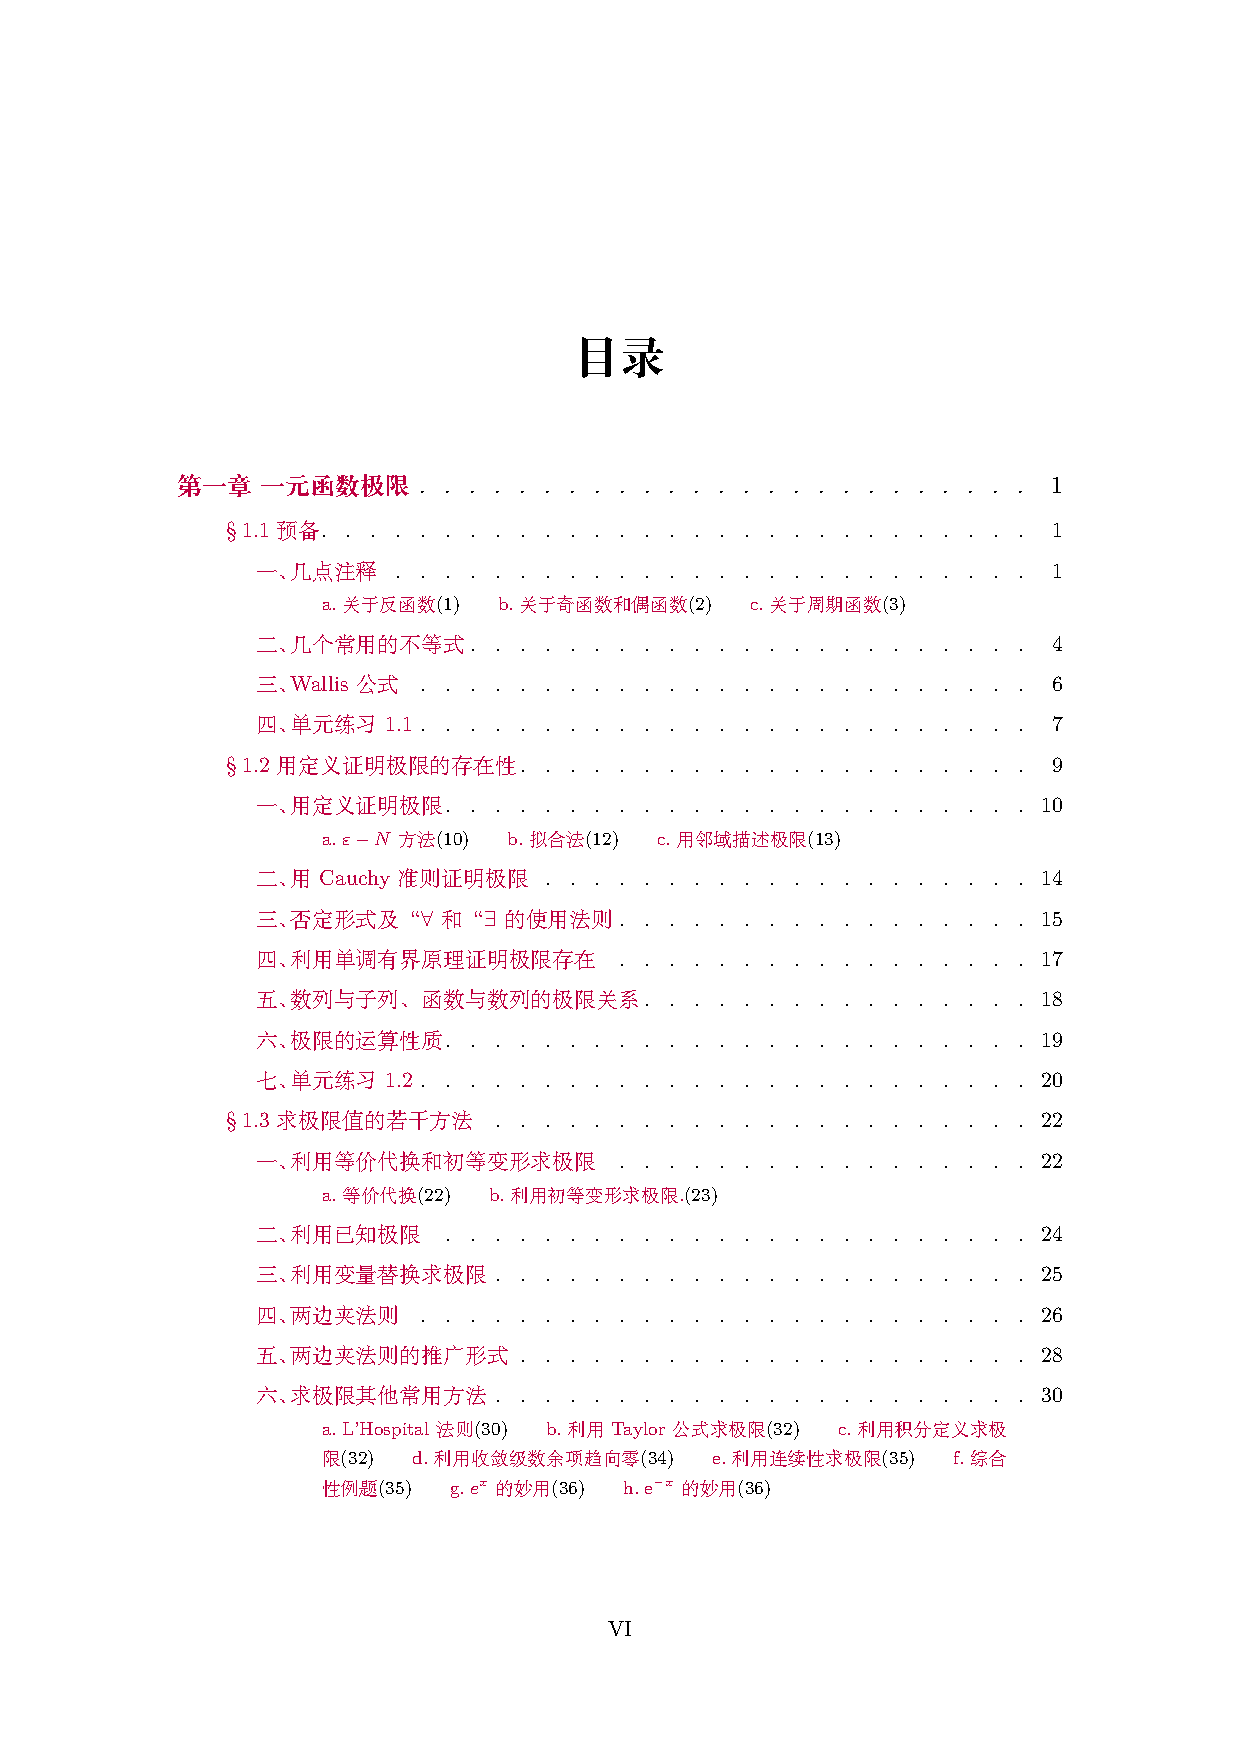
\includegraphics[width=.32\linewidth]{./pics/ToC_1.pdf}
    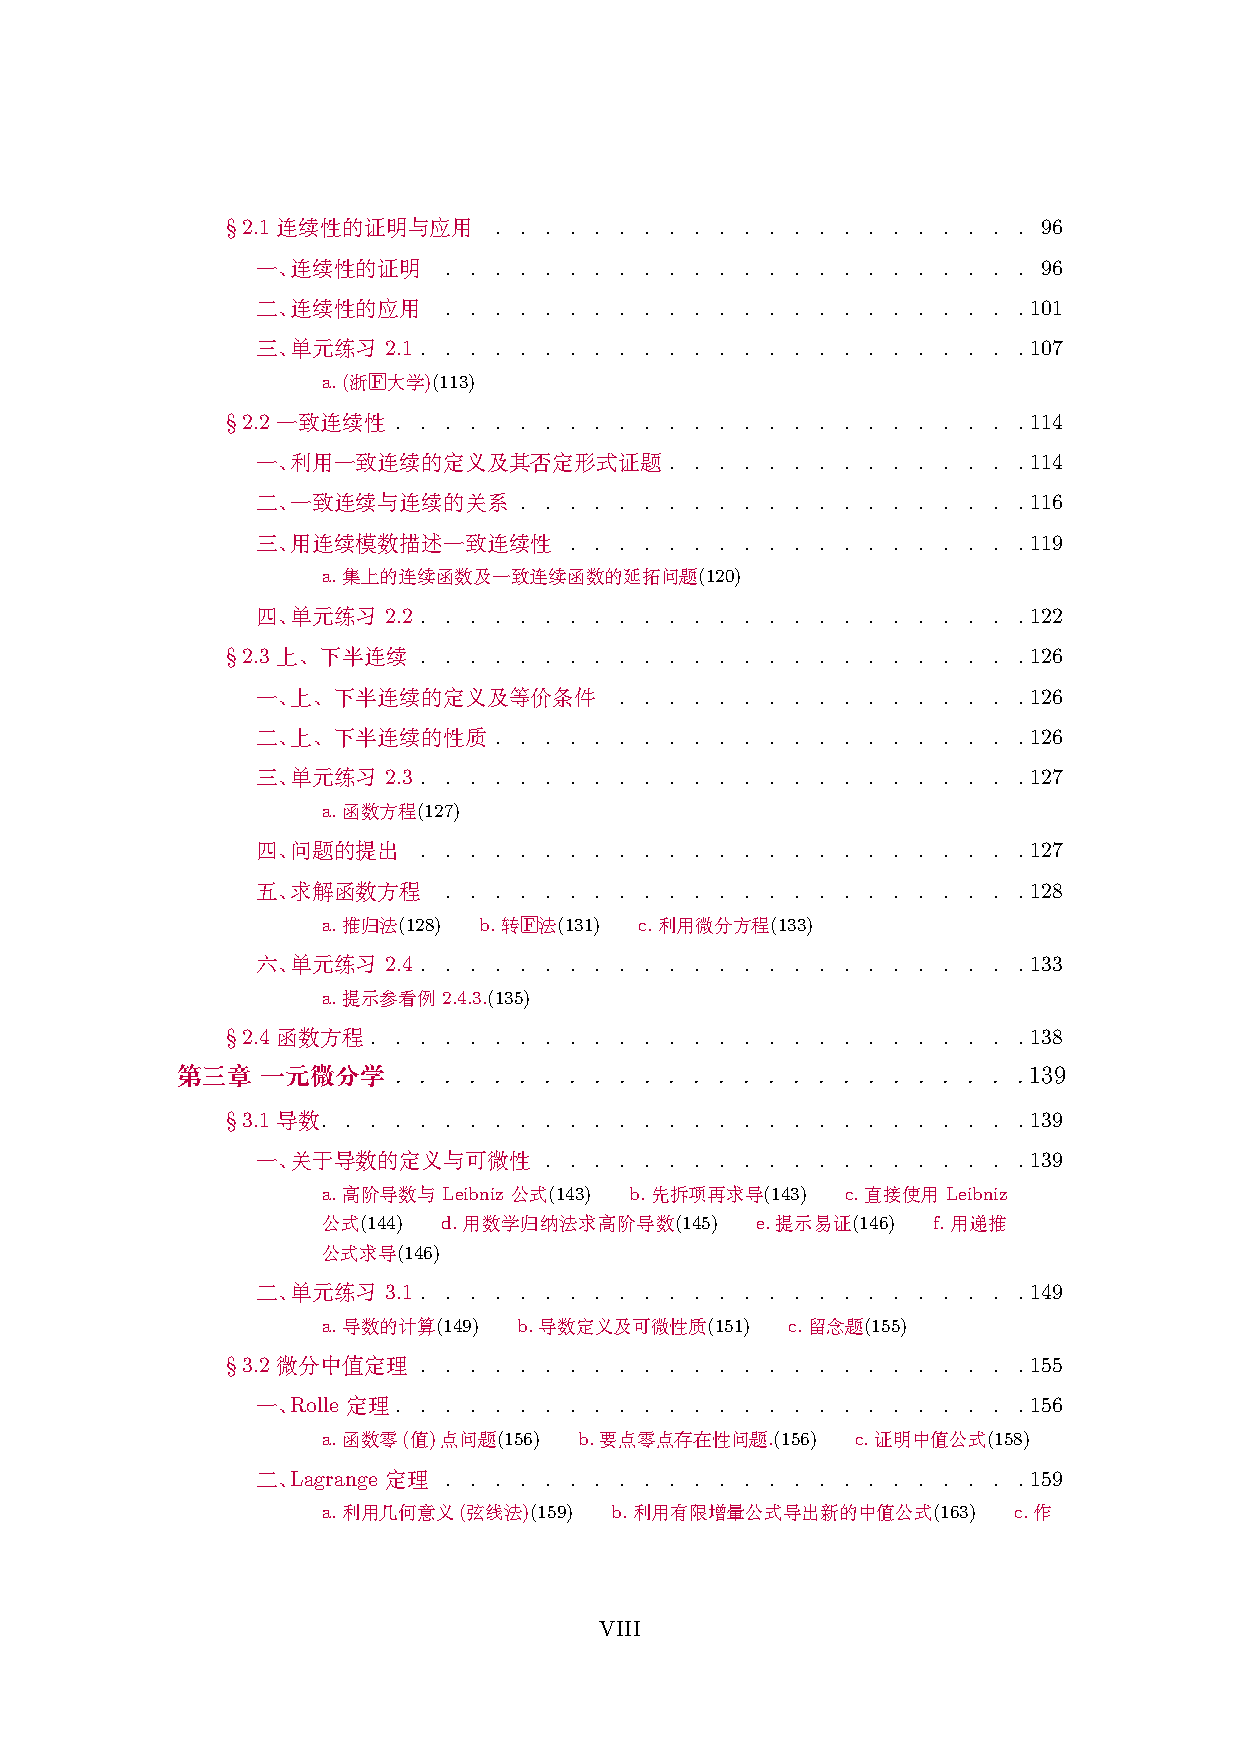
\includegraphics[width=.32\linewidth]{./pics/ToC_2.pdf}
    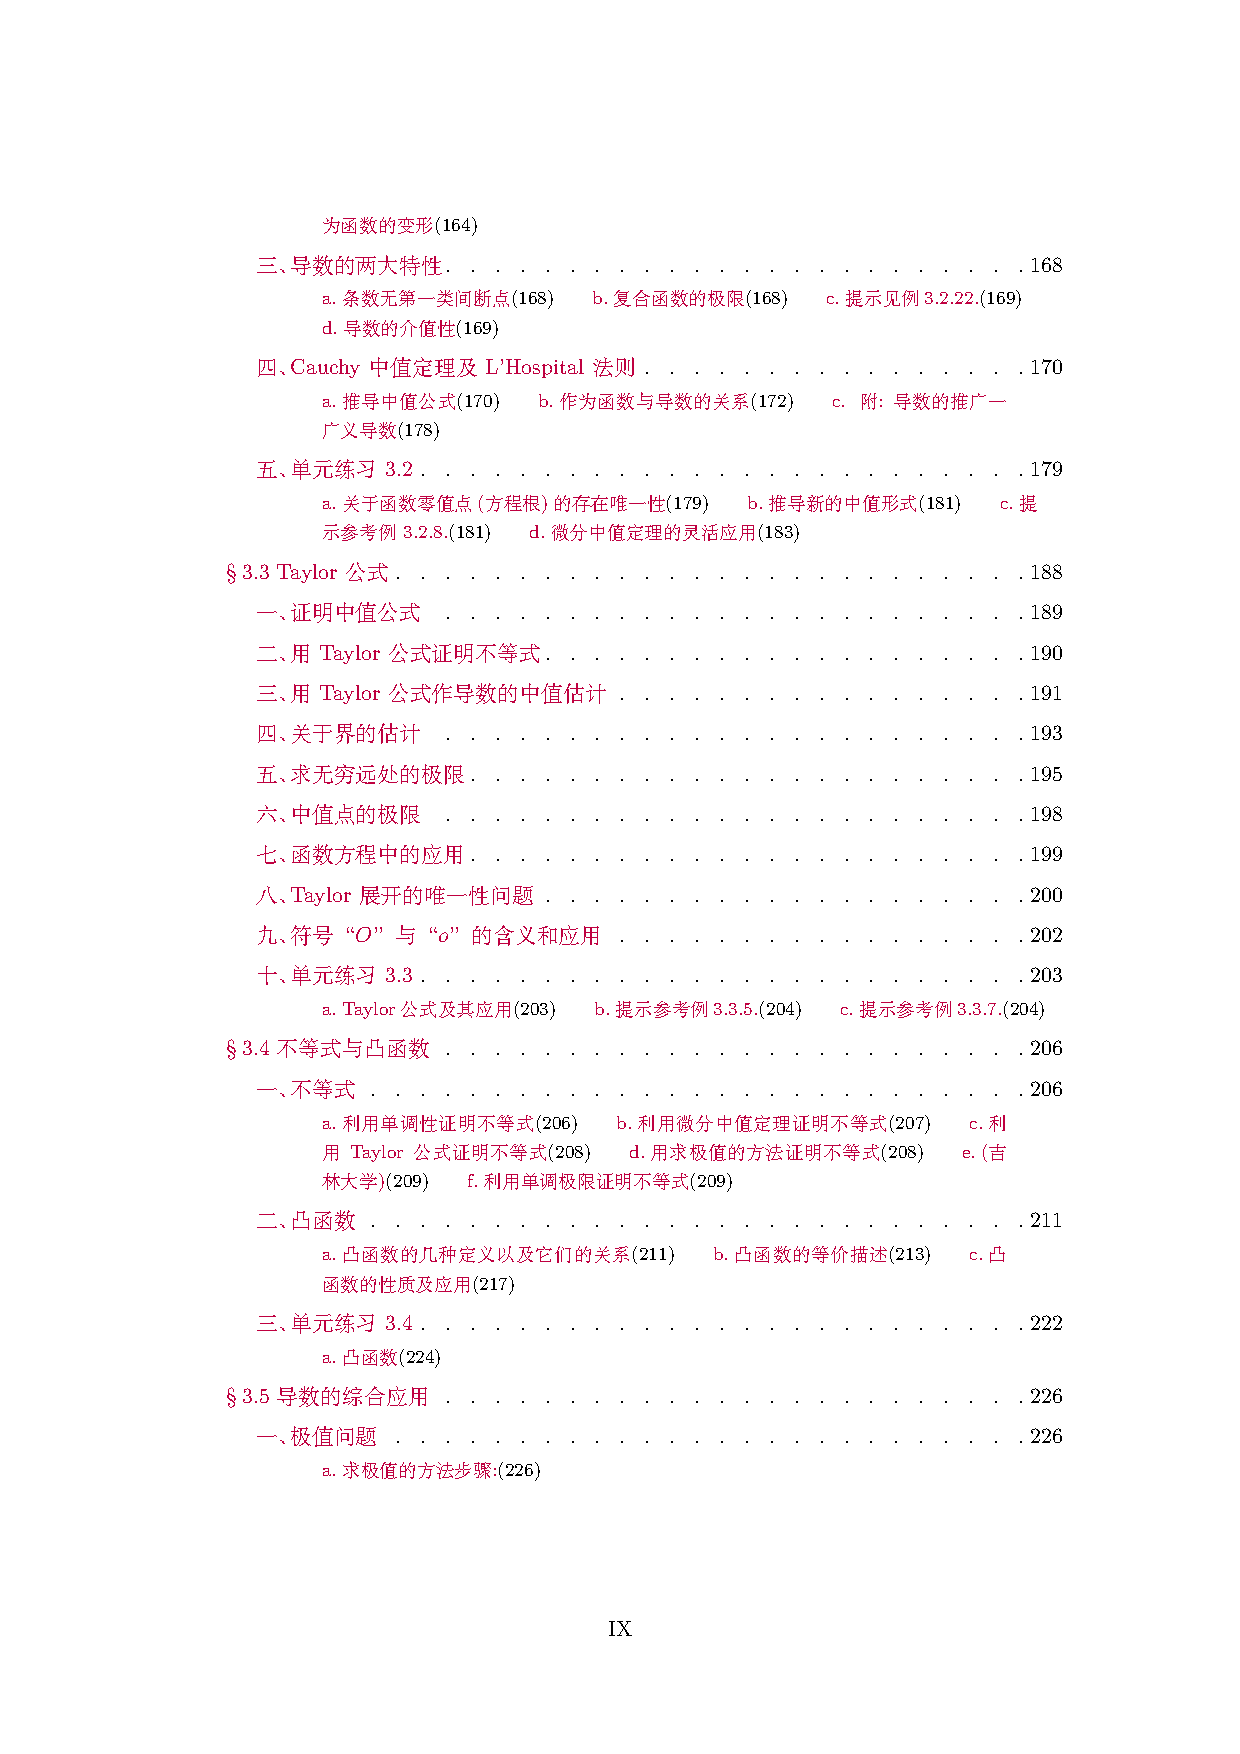
\includegraphics[width=.32\linewidth]{./pics/ToC_3.pdf} 
    \caption{ToC Example}
    \label{fig:toc-example}
\end{figure}


\begin{leftbar}
本文档类默认不加载 {tikz, pgf} 宏包,想要使用这两个宏包定义更加复杂章节样式,请手动加载,并设置自己喜欢的章节格式. 
也许后续我会在 z\LaTeX{} 的加载选项中添加一个 tikz 宏包选项,从而可以让用户自定义章节格式.
\end{leftbar}

\section{字体配置}\index{font-config}\label{font-config}
\subsection{一些术语}
在字体上,国内环境可以说是一团浆糊,再加之M\$ word对用户的不断误导与溺爱,导致无数的用户不知道字体,字体族,
字体系列,字形的区别. 下面给出一些常见注意事项:
\begin{itemize}
    \item 可以粗略的认为一个字体中包含了一些字体族,一些字体系列. 做字体是一个吃力不讨好的活,没多少人愿意做.
    \item 一般这个字形是对于西文字体而言的,对于中文无效. 中文所谓的斜体概念都是 word 这个毒瘤产生的.
      部分字体本来就不是给中文设计的,所以不要想着把它们应用在中文上.
    \item 深受M\$ Office迫害的用户很多喜欢Times New Roman字体,但是它并没有对应的数学字体(\cmd{newtxmath}不是).
    \item \textbf{注意字体版权:} Windows默认的字体全部都是有商业版权的.原则上,只有正版Windows用户方才可以用于非商业用途.如需用于商业,必须获得授权
\end{itemize} 

\subsection{New Computer Modern}
目前在 Xe\TeX{} 下已有一个比较完善的字体包 \cmd{newcomputermodern}\index{\cmd{newcomputermodern}},这个包 
兼容原始的 CM 字体,并且对部分的细节进行了优化. 最重要的是,它支持多种语言:希腊语,俄语,中文,日文,韩文,西里尔语和梵文等.
这个包的使用方法如下:

\begin{minted}{latex}
% way 1
\usepackage{newcomputermodern}

% way 2
\usepackage[default]{fontsetup}
\end{minted}

推荐使用第二种方式进行调用, 具体的使用细节请参见:\href{https://ctan.org/pkg/newcomputermodern}{New Computer Modern}.

\subsection{模板预设}\index{模板字体预设}
字体配置一直以来都是一个比较头疼的问题,尤其是对于中文文档. z\LaTeX{}目前具有两套字体设置:英文和中文.
英文(\cmd{lang=en})下的字体配置为:
\begin{minted}{latex}
\RequirePackage[utf8]{inputenc}
\RequirePackage[T1]{fontenc}
\RequirePackage[english]{babel} 
\end{minted}

在中文(\cmd{lang=cn})环境下的字体配置为:
\begin{minted}{latex}
\RequirePackage[UTF8, heading]{ctex}
% 如果加载了ctexbook则为:
\LoadClass[oneside, 11pt]{book}
\end{minted}

除了上述的设置外,本模板目前没有进行任何多余的字体配置. 但是为了方便用户,后续,可能,z\LaTeX{} 会提供一个
\cmd{\zlatexFontSetup}\index{\cmd{\zlatexFontSetup}} 命令进行不同系统上的字体配置, 以及文档中:正文字体,数学字体
等的配置. 但在此命令写好之前,这里首先介绍如何 \LaTeX{} 中调用外部字体或者是系统字体,毕竟这个才是大多数用户的需求.

\subsection{查看系统字体}\index{查看系统字体}
首先介绍正文字体,正文字体的设置基于\cmd{fontspec}宏包, 可以解决在 \hologo{XeLaTeX}, \hologo{LuaLaTeX}下的字体配置问题.此宏包提供了如下
命令用于正文中各种字体族的设置\index{\cmd{\setmainfont}}\index{\cmd{\setsansfont}}\index{\cmd{\setmonofont}}:
\begin{itemize}
    \item \cmd{\setmainfont}: 设置正文的主要字体(罗马字体), 对应命令\cmd{\textrm}
    \item \cmd{\setsansfont}: 设置正文的无衬线字体, 对应命令\cmd{\textsf}
    \item \cmd{\setmonofont}: 设置正文的等宽字体(打字机字体), 对应命令\cmd{\texttt}
\end{itemize}

\begin{leftbar}
如果想要在pdf\TeX{}下使用别的字体(你自己下载的字体,系统中别的字体),那么最好的方法是使用别人写好的宏包.因为
在pdf\TeX{}下使用别的字体,可能会需要一些\cmd{.tfm, .fd, .map, .sty}等文件,这个对于一般的\LaTeX{}使用者来说过于复杂了.
可以参见网站:\href{https://tug.org/FontCatalogue/allfonts.html}{FontCatalogue}, 在这个网站上你可以看到很多的为pdf\TeX{}
设计的字体宏包,然后你根据自己的喜好进行对应宏包的设置即可.
\end{leftbar}

\begin{figure}[!htb]
    \centering
    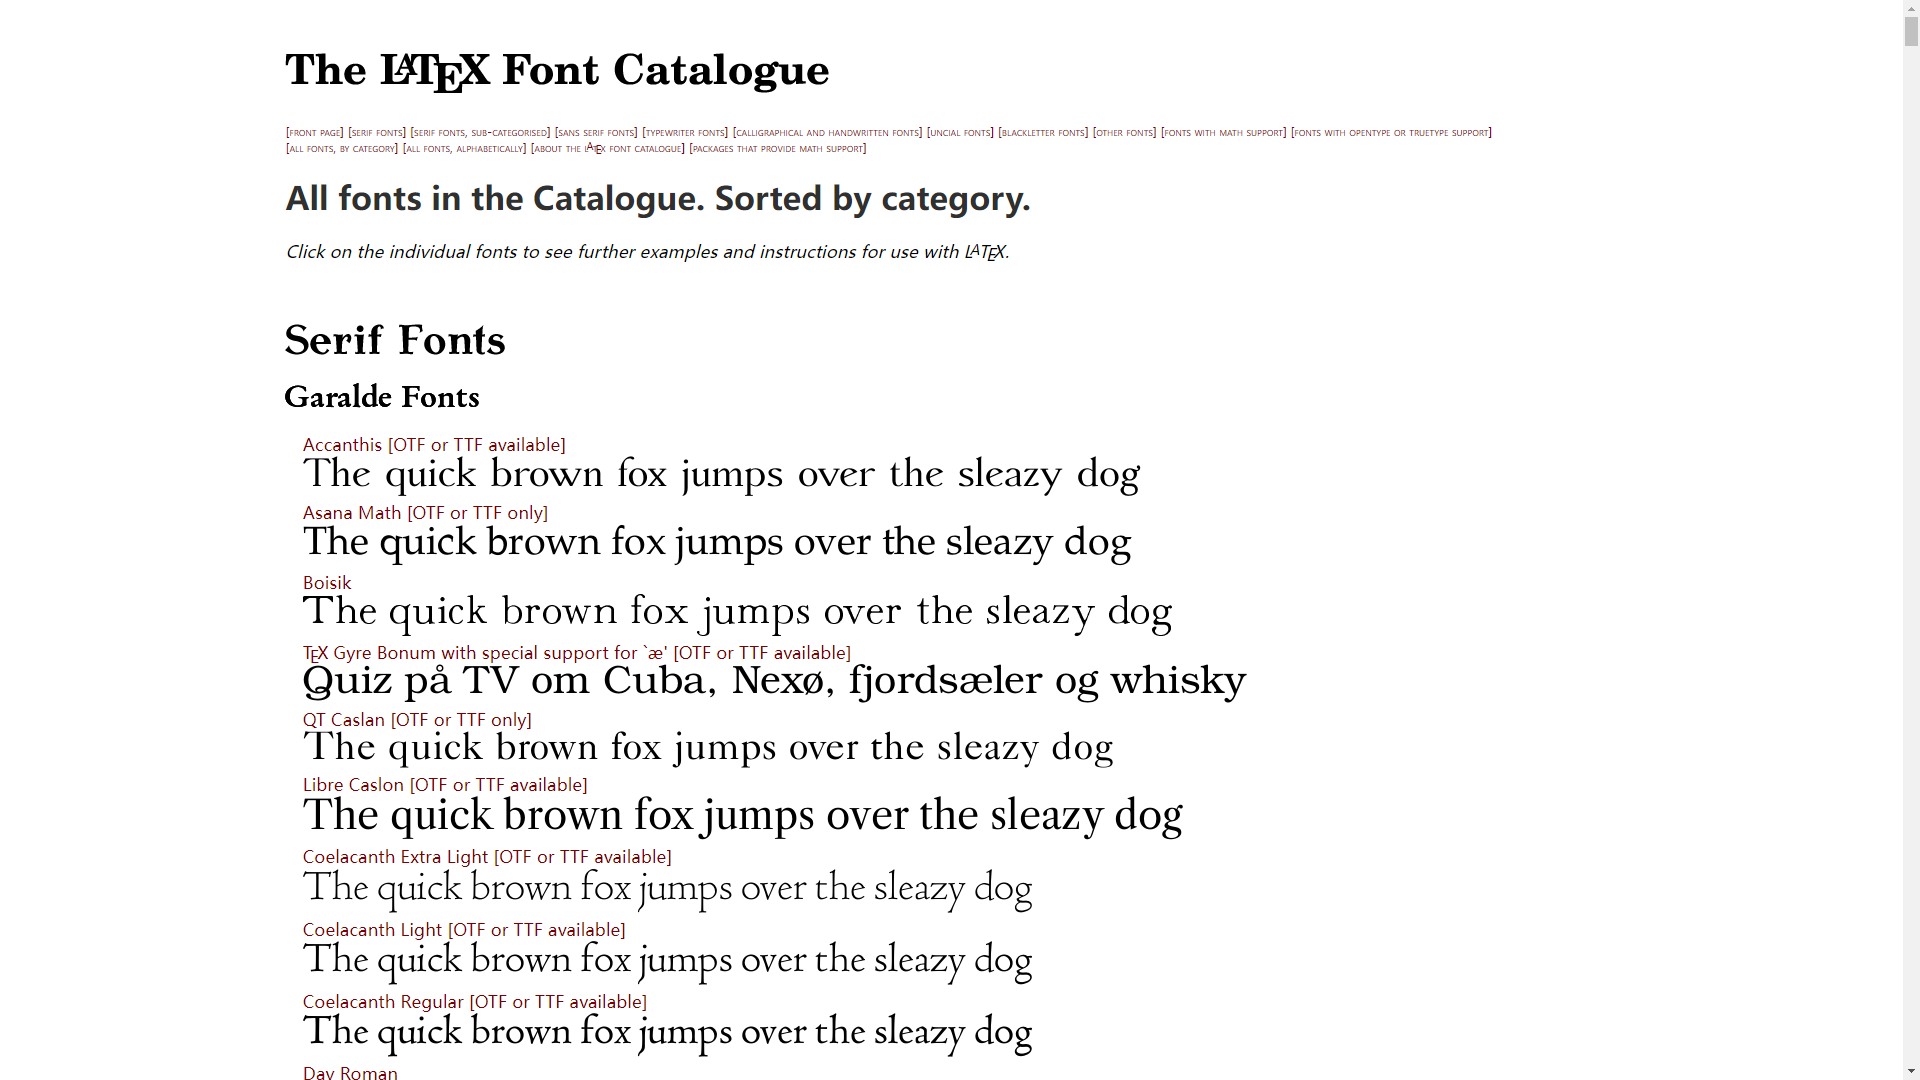
\includegraphics[width=.75\linewidth]{./pics/pdftex_font_config.png}
    \caption{Font Catalogue}
    \label{fig:FontCatalogue}
\end{figure}


\begin{leftbar}
在设置全文的中(日韩)字体时也请使用命令\cmd{\setCJKmainfont}命令,格式和上述的命令一样. 也许在设置文档的中文字体时你还需要在导言区
加载如下命令:
\end{leftbar}
\begin{minted}{latex}
\renewcommand\CJKrmdefault{}
\end{minted}

这几个命令可以用于设置整个文档的字体,但是同样的是,我们可以在一个文档中使用多个字体. 在讨论这个的时候,
我们遇到了一个问题? 怎么查看自己电脑上有哪些可用的字体(包括数学字体)? 在Windows和Linux均可以通过如下命令进行
查看:
\begin{minted}{shell}
fc-list 
\end{minted}

然后你就会看到如下的类似输出, 在Linux下可能是这样的:
\begin{minted}{text}
/usr/share/fonts/100dpi/lubI24.pcf.gz: B&H LucidaBright:style=Italic
/usr/share/fonts/100dpi/UTBI__12-ISO8859-1.pcf.gz: Adobe Utopia:style=Bold Italic
/usr/share/fonts/75dpi/luIS08-ISO8859-1.pcf.gz: B&H Lucida:style=Sans Italic
/usr/share/fonts/75dpi/luIS10-ISO8859-1.pcf.gz: B&H Lucida:style=Sans Italic
/usr/share/fonts/75dpi/luIS14-ISO8859-1.pcf.gz: B&H Lucida:style=Sans Italic
/usr/share/fonts/100dpi/luRS18-ISO8859-1.pcf.gz: B&H Lucida:style=Sans
/usr/share/fonts/75dpi/courB18-ISO8859-1.pcf.gz: Adobe Courier:style=Bold
/usr/share/fonts/100dpi/lubBI24.pcf.gz: B&H LucidaBright:style=Italic
/usr/share/fonts/100dpi/courO12.pcf.gz: Adobe Courier:style=Oblique
\end{minted}

在windows上可能是这样的(如果安装了\TeX{}Live):
\begin{minted}{text}
C:/WINDOWS/fonts/times.ttf: Times New Roman:style=Regular,Normal, ...
C:/WINDOWS/fonts/GeoSlab703 Md BT Bold.ttf: GeoSlab703 Md BT:style=Bold
C:/WINDOWS/fonts/vgasysr.fon: System:style=Regular
C:/WINDOWS/fonts/seguibl.ttf: Segoe UI,Segoe UI Black:style=Black,Regular
C:/texlive/2024/texmf-dist/fonts/opentype/public/drm/drmsl11.otf: drmsl11:style=Regular
C:/texlive/2024/texmf-dist/fonts/opentype/public/fonts-tlwg/Garuda-Oblique.otf: Garuda:style=Oblique
C:/texlive/2024/texmf-dist/fonts/truetype/public/junicodevf/JunicodeVF-Roman.ttf: Junicode VF:style=Exp Bold
C:/texlive/2024/texmf-dist/fonts/opentype/public/qualitype/QTTechtone-BoldItalic.otf: QTTechtone:style=BoldItalic
C:/texlive/2024/texmf-dist/fonts/opentype/public/tempora/Tempora-Italic.otf: Tempora:style=Italic
C:/texlive/2024/texmf-dist/fonts/opentype/public/drm/drmsym11.otf: drmsym11:style=Regular
\end{minted}

我们可以通过 ``font name'' 和  ``file name'' 两种形式来调用字体. 比如我们想要调用 ``Times New Roman'' 字体,
在第一个输出示例中,可以看到 ``Times New Roman'' 对应的文件名为 ``times.ttf'', 那么我们可以通过如下命令进行调用:
\begin{minted}{latex}
% by file name 
\setmainfont{times.ttf}

% by font name
\setmainfont{Times New Roman}
\end{minted}

\begin{leftbar}
如果你不想在你的本地安装过多的字体,我常常会建议使用``file name''的格式.只需要把对应的字体文件放到你的项目文件夹下就行了,
免去了字体安装这一个步骤.这个时候你就需要在可选参数中指定键\zkey{Path}对应的路径值,对应的是项目下的字体路径. 这里给出一个示例:
假如你把字体放到了项目根路径下的 {Fonts} 文件夹,那么声明格式为:
\end{leftbar}
\begin{minted}{latex}
\setmainfont[Path = Fonts/]{<font name or file name>}
\end{minted}

在安装字体后务必使用如下命令刷新系统字体缓存,否则 {fontspec}或 {xeCJK}宏包无法找到系统中对应的字体:
\begin{minted}{shell}
fc-cache -f -v
\end{minted}

通过上面的两条命令我们便可以轻松的设置文档中\cmd[F]{\textrm{<content>}}对应的字体\Footnote{默认情况下,文档中的字体族即为roman family}
为``Times New Roman''.

\subsection{读懂字体警告}\index{字体系列}
但是你可能也会遇到如下的编译警告:
\begin{minted}{text}
LaTeX Font: Font shape `TU/AlegreyaSans-ExtraBoldItalic.otf(0)/b/n' undefined
(Font)	using `TU/AlegreyaSans-ExtraBoldItalic.otf(0)/m/n' instead.
\end{minted}

上述的字体是我在导言区设置了如下字体命令导致的:
\begin{minted}{latex}
\setmainfont{AlegreyaSans-ExtraBoldItalic.otf}
\end{minted}

为什么会有这个警告? 其实就是出在一个字体加粗命令\cmd{\textbf}上,我并没有指定这个新的文章中字体族(rmfamily)所对应的
粗体系列字体. 所以\TeX{}采用了默认的 ``m(edium)'', 而不是 ``b(old)''. 详细信息可以参见\cite{goossens1994latex}:
The \LaTeX{} Companion(3rd) -- Font Selection and Encodings. 这里给出其中两个关于关于字体设置的表格:

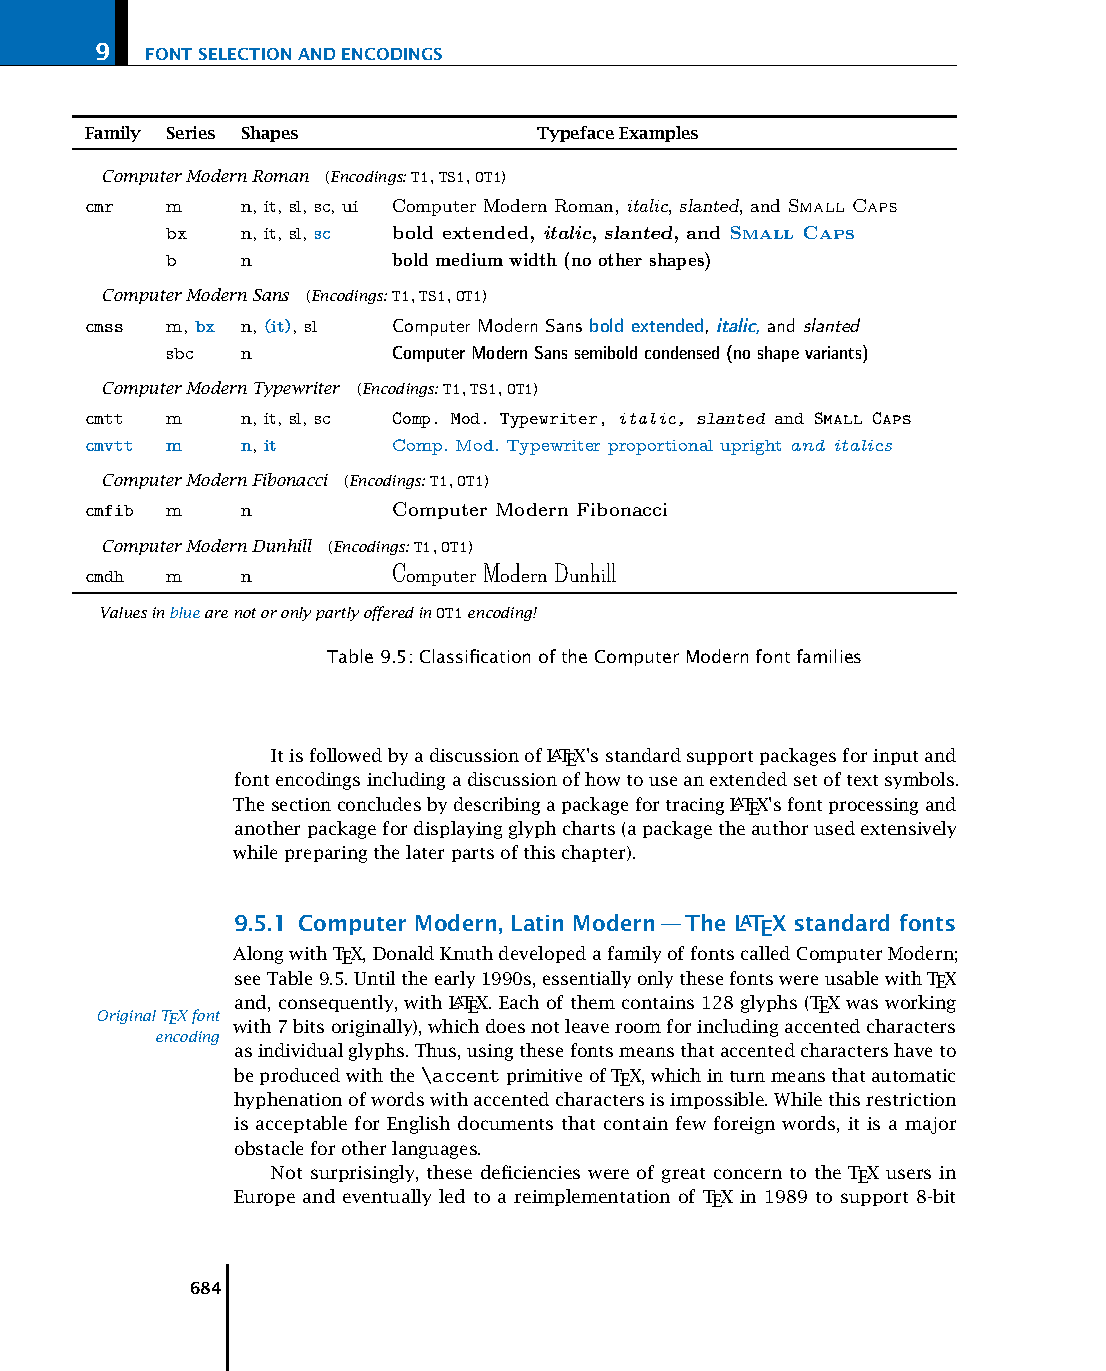
\includepdf{./pics/cmr.pdf}
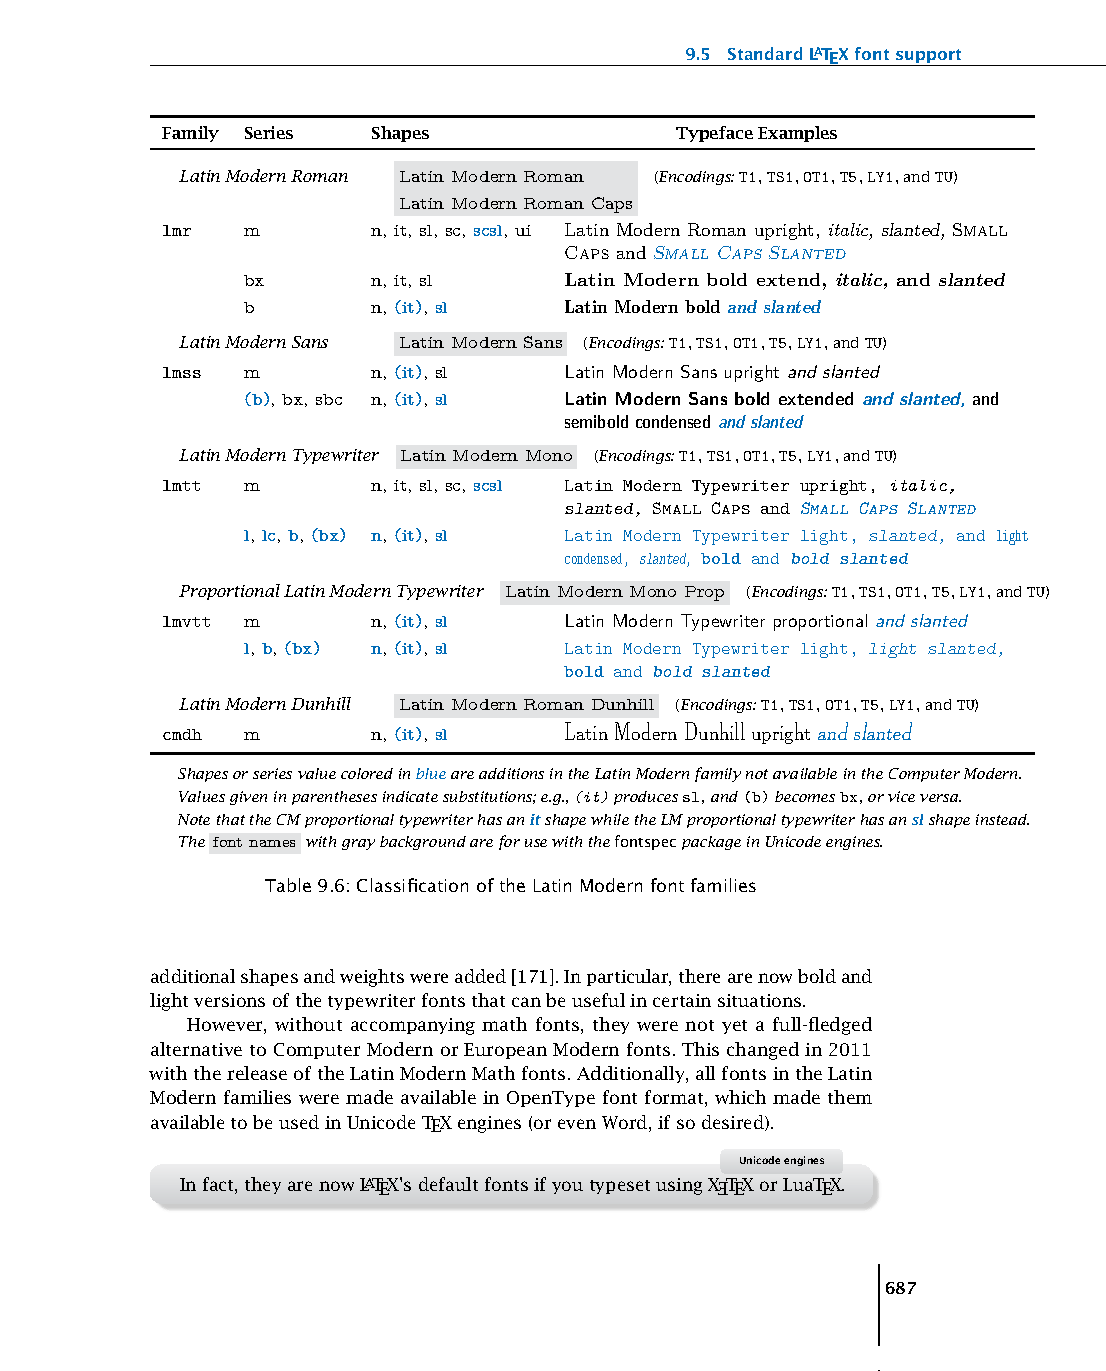
\includepdf{./pics/lmr.pdf}


在阅读了上述关于``字体的选择''内容之后,解决这个问题就不难了,给出两个方法:
\begin{itemize}
    \item 通过``font name''进行设置的情况下,如果你的本地字库够全,那么\TeX{}会自动处理这个问题.
    \item 通过``file name''进行设置的情况下,你可以通过如下命令进行设置,这里以\cmd{comic.ttf}为例:
\end{itemize}

\begin{minted}{latex}
\setmainfont{comic.ttf}[
    BoldFont=comicbd.ttf,
    ItalicFont=comici.ttf,
    BoldItalicFont=comicz.ttf
]
\end{minted}

如果你在Windows命令行使用如下命令:
\begin{minted}{shell}
fc-list | rg comic | rg WINDOWS
\end{minted}

那么可以得到如下的输出:
\begin{minted}{shell}
C:/WINDOWS/fonts/comicbd.ttf: Comic Sans MS:style=Bold
C:/WINDOWS/fonts/comici.ttf: Comic Sans MS:style=Italic
C:/WINDOWS/fonts/comicz.ttf: Comic Sans MS:style=Bold Italic
\end{minted}

说明在本地的名为``Comic Sans MS''的字体族具有``Bold, Italic, Bold Italic''三种字形. 通过下面的命令我们便可以
简单的通过第一种方式解决这个字体加粗问题:
\begin{minted}{latex}
\setmainfont{Comic Sans MS}
\end{minted}

\begin{leftbar}%
就像上述备注的第二种``file name''方式的好处外,By ``font name'' 也有上述的优点. 尽管对于字体的加粗和斜体你可以偷懒,
在字体族声明的可选参数中加入\cmd{AutoFakeBold, AutoFakeSlant}参数,它会自动同时实现中英文伪粗体和伪斜体,不用你自己单独去指定.
但是我并不推荐. 还是给出一个示例:
\end{leftbar}

\begin{minted}{latex}
\setCJKfamilyfont{AutoFakeBoldSlant}{<font-name>.ttf}[AutoFakeBold , AutoFakeSlant]
\end{minted}

在通过 ``font name''进行字体的声明时,可以考虑把字体放到如下的位置,这样可以避免书写字体的路径:
\begin{itemize}
    \item MacOS:\cmd[F]{~/Library/Fonts}
    \item Windows:\cmd[F]{C:\Windows\Fonts}
    \item Linux 或 Windows: 放在TEXMF tree对应的路径, 见前文.
\end{itemize}

\subsection{字体族声明}\index{字体族声明}
上述的三个命令都是设置全文对应的字体族,如果你想要改变局部的字体族,那么可以使用\cmd{fontspec}宏包提供的
命令\cmd{\newfontfamily}和\cmd{XeCJK}宏包提供的\cmd{\setCJKfamilyfont}分别进行英文与中日韩文字的字体族声明.
二者的声明方式为:
\begin{minted}{latex}
\newfontfamily{\FamilyA}{FontA.ttf}
\setCJKfamilyfont{FamilyB}{FontB.ttf}
\end{minted}

上述两条命令声明了\cmd{FamilyA, FamilyB}两个字体族,分别对应了\cmd{FontA.ttf, FontB.ttf}两个字体文件.想要使用
这两个字体族,在文档中按照如下方式使用:
\begin{minted}{latex}
{\FamilyA <Your Content>}
{\CJKfamily{FamilyB} <你的内容>}
\end{minted}

比如你需要在文档中输入俄语,由于\cmd{article}文档类默认的字体Computer modern并没有包含这些俄语字母字形(Glyph).
所以你可能就需要使用一个含有这类字形的字体了,推荐\cmd{CMU Serif}.可以安装进系统也可以放在项目文件夹下,这里放在
项目文件夹\cmd{./Fonts/}下为例:
\begin{minted}{latex}
\newfontfamily{\russia}[Path=./Fonts/]{cmunrm.ttf}[
    BoldFont=cmunbx.ttf,
    ItalicFont=cmunbi.ttf
]
\end{minted}

然后使用如下格式调用:
\begin{minted}{latex}
{\russia <俄语内容>}
\end{minted}

\begin{leftbar}
{\russia Жизнь, как прекрасная мелодия, только текст перепутались.}\par 
\noindent{\kaishu 生命是首美丽的曲子,只是歌词有些纠结}
\end{leftbar}


当然了,你也可以通过\cmd{\setmainfont}命令,从而进行全局字体设置. 最后还是给出声明中文字体族的一个简单示例:
\begin{minted}{latex}
\setCJKfamilyfont{fangsong}{simfang.ttf}[
    Path=./Fonts/,
    BoldFont=simfangbold.ttf
]
\end{minted}

在声明了对应的字体族之后,使用如下格式进行调用:
\begin{minted}{latex}
{\CJKfamily{fangsong} <你的中文内容>}
\end{minted}

\subsection{Emoji}\index{Emoji}
如果用户想要使用Emoji,在阅读完上述的字体配置后,相信读者已经能够独自解决此问题了. 这里给出大致的解决思路:
\begin{itemize}
    \item 把对应的Emoji对应的unicode放到一个支持显示表情包的字体组环境中.
    \item 加载 \href{http://mirrors.ctan.org/fonts/fontawesome5/doc/fontawesome5.pdf}{fontawesome5} 宏包.
    \item 更换编译引擎为 \hologo{LuaTeX}.
\end{itemize}


\subsection{数学字体}\label{数学字体}\index{数学字体}
目前z\LaTeX{}文档类提供了几种常见的数学字体宏包接口,分别是 {computer moder math, newtxmath, eulervm, mtpro2}. 
其中\cmd{computer modern math} 即为默认的数学字体,推荐刚上手的用户使用. 这里需要说明:数学字体并不仅仅只包含我们直接看到的
那部分Glyph本身,一套数学字体往往还需要对应的一个kern tables(距离表),用于指定各个数学符号之间的距离. 数学字体还包含很多复杂的东西,
并没有我们认为的那么简单.

不想要折腾的用户可以直接看 \href{http://mirrors.ctan.org/info/Free_Math_Font_Survey/en/survey.pdf}{Free-Math-Font} 这个 
文档, 其中提供了多种数学字体的调用方法.即使是你配置不来,但是至少你能够直接参考文档中的案例实现自己的需求.但这里不去介绍上述对应宏包
的使用方法,下面重点介绍宏包\href{http://mirrors.ctan.org/macros/unicodetex/latex/unicode-math/unicode-math.pdf}{unicode-math}. 

\cmd{unicode-math}\index{\cmd{unicode-math}}宏包的基本使用格式为:
\begin{minted}{latex}
% after \usepackage{fontspec}
\usepackage{unicode-math}
% set main math font (necessary)
\setmathfont{Latin Modern Math}
\end{minted}

上述的命令\cmd{\setmathfont}\index{\cmd{\setmathfont}}由宏包\cmd{unicode-math}提供,用于设置文档中数学字体. 在指定文档的数学字体后,你可以
再声明一系列的数学字体命令用于指定局部数学字体样式. 但是在这之前,请允许我先介绍一下怎么查看你本地系统中的数学字体. 

以 Windows 为例,在命令行运行:
\begin{minted}{shell}
fc-list | rg Math
\end{minted}

然后你可以得到大致如下的结果:
\begin{minted}{text}
C:/WINDOWS/fonts/eumat2.ttf: Euclid Math Two:style=Regular
C:/WINDOWS/fonts/eumat2b.ttf: Euclid Math Two:style=Bold
C:/WINDOWS/fonts/cambria.ttc: Cambria Math:style=Regular
C:/texlive/2024/texmf-dist/fonts/opentype/public/xits/XITSMath-Bold.otf: XITS Math:style=Bold
C:/texlive/2024/texmf-dist/fonts/opentype/public/xits/XITSMath-Regular.otf: XITS Math:style=Regular
C:/texlive/2024/texmf-dist/fonts/opentype/public/tex-gyre-math/texgyretermes-math.otf: TeX Gyre Termes Math:style=Regular
\end{minted}

和前文的设置正文字体一样,可以通过``font name'' 或者是 ``file name''进行数学字体的设置, 所以在这里不再赘述. 
这里介绍一下怎么设置局部数学字体. 通过如下命令:
\begin{minted}{latex}
\setmathfont[range={\mathscr,\mathbfscr}]{TeX Gyre Termes Math}
\end{minted}

在此命令之后的所有\cmd[F]{\mathscr, \mathbfscr}命令均会使用``TeX Gyre Termes Math''字体. 其他不变, 比如\cmd[F]{\mathrm, \mathbf}等.
后续如果还想使用其他数学字体,只需要再次声明不同的\cmd[F]{\setmathfont}命令即可.

\begin{leftbar}
值得注意的是:在加载宏包\cmd{unicode-math}后,数学字符的加粗请采用\cmd[F]{\boldsymbol}或\cmd[F]{\symbf, \symbfit, \symbfup}等命令.
\end{leftbar}

关于\cmd{unicode-math}宏包的更多功能,请参见对应的宏包手册. 


\subsection{常见字体问题}\index{常见字体问题}
在阅读了上述字体配置的基础知识介绍后,你应该能看懂大部分模板中的字体配置了. 在看懂这些命令后,也就能够说明一些常见字体问题
背后原因了:
\begin{itemize}
    \item 为什么 Windows 下中文加粗变成了黑体? 斜体变成了楷体?
    \item 为什么有时 \LaTeX{} 会报字体缺失的警告或错误?
    \item 怎么在 Windows 上使用 Linux 下的字体? 或者反过来使用 ?
    \item 怎么使用 Founder 字体 ?
    \item ...
\end{itemize}

在 Windows 下文字加粗后变黑体的问题\Footnote{具体参考请见:\href{https://zhuanlan.zhihu.com/p/538459335}{LaTeX 中文字体配置基础指南}},
如果你去看\cmd{ctex-fontset-windows.def}这个文件,有如下声明:
\begin{minted}{latex}
% 中文默认字体:宋体,粗体以黑体代替,斜体以楷书代替
\setCJKmainfont   { SimSun } [ BoldFont = SimHei , ItalicFont = KaiTi ]
% 中文无衬线字体:微软雅黑,粗体为对应的微软雅黑粗体
\setCJKsansfont   { Microsoft~YaHei } [ BoldFont = *~Bold ]
% 中文等宽字体:仿宋
\setCJKmonofont   { FangSong }
% 设置中文字族
\setCJKfamilyfont { zhsong  } { SimSun          }
\setCJKfamilyfont { zhhei   } { SimHei          }
\setCJKfamilyfont { zhfs    } { FangSong        }
\setCJKfamilyfont { zhkai   } { KaiTi           }
\setCJKfamilyfont { zhyahei } { Microsoft~YaHei } [ BoldFont = *~Bold ]
\setCJKfamilyfont { zhli    } { LiSu            }
\setCJKfamilyfont { zhyou   } { YouYuan         }
% 字体命令,可用于文档中自由设置字体
\NewDocumentCommand \songti   { } { \CJKfamily { zhsong  } }
\NewDocumentCommand \heiti    { } { \CJKfamily { zhhei   } }
\NewDocumentCommand \fangsong { } { \CJKfamily { zhfs    } }
\NewDocumentCommand \kaishu   { } { \CJKfamily { zhkai   } }
\NewDocumentCommand \lishu    { } { \CJKfamily { zhli    } }
\NewDocumentCommand \youyuan  { } { \CJKfamily { zhyou   } }
\NewDocumentCommand \yahei    { } { \CJKfamily { zhyahei } }
\end{minted}

上面有一句\cmd{BoldFont = SimHei}, 就表示\cmd[F]{\textbf{<文字>}}中的内容是``黑体''.但是在Linux下对应的设置为:
\texttt{BoldFont = FandolSong-Bold},这就是真正的 fandol 字体中的粗体了.

比如Elegant\LaTeX{}系列中的Book文档类,你能在其中看到如下的字体声明命令:
\begin{minted}{latex}
% 英文部分
\setmainfont{TeXGyreTermesX}[
    UprightFont = *-Regular ,
    BoldFont = *-Bold ,
    ItalicFont = *-Italic ,
    BoldItalicFont = *-BoldItalic ,
    Extension = .otf ,
    Scale = 1.0
]
\setsansfont{texgyreheros}[
    UprightFont = *-regular ,
    BoldFont = *-bold ,
    ItalicFont = *-italic ,
    BoldItalicFont = *-bolditalic ,
    Extension = .otf ,
    Scale = 0.9
]

% 中文部分
\RequirePackage[UTF8, scheme=plain, fontset=none]{ctex}
\setCJKmainfont[BoldFont={FZHei-B01},ItalicFont={FZKai-Z03}]{FZShuSong-Z01}
\setCJKsansfont[BoldFont={FZHei-B01}]{FZKai-Z03}
\setCJKmonofont[BoldFont={FZHei-B01}]{FZFangSong-Z02}
\setCJKfamilyfont{zhsong}{FZShuSong-Z01}
\setCJKfamilyfont{zhhei}{FZHei-B01}
\setCJKfamilyfont{zhkai}[BoldFont={FZHei-B01}]{FZKai-Z03}
\setCJKfamilyfont{zhfs}[BoldFont={FZHei-B01}]{FZFangSong-Z02}
\newcommand*{\songti}{\CJKfamily{zhsong}}
\newcommand*{\heiti}{\CJKfamily{zhhei}}
\newcommand*{\kaishu}{\CJKfamily{zhkai}}
\newcommand*{\fangsong}{\CJKfamily{zhfs}}
\end{minted}

所以C\TeX{}还是给我们解决了很多的字体问题的,如果你的文档中加载了\cmd{ctex}宏包,不妨使用其提供的\cmd{<fontset>}
选项进行字体的设置. 实在不行,再考虑自行配置字体也不迟.

\subsection{Furthermore}
本节并没有介绍在pdf\TeX{}下的字体配置方法,因为如果你想在此引擎下使用字体,那么你可能需要自己去做一些复杂的字体工作,
自己去做对应的\texttt{tfm, map, enc, vf}文件,这并不简单. 

还有一些 FallBack字体(主字体文件中不存在字符的备用字体)的问题? 比如在 Windows 下可以使用其自带的一个超大字符集\cmd{SimSun-ExtB},
设置方法如下:
\begin{minted}{latex}
\xeCJKsetup{AutoFallBack=true}
\setCJKmainfont{SimSun}[FallBack=SimSun-ExtB]
\end{minted}

什么,你还想了解 PDF 的知识? 或者是虚拟字体相关的工作? 这些都不是我们一般人能够去碰的, 如果你想要了解更多字体相关的知识,
不妨就局限在宏包调用的水平, 可以多看看 {fontspec, ctex} 相关的文档, 或者是看看 {The \LaTeX{} Companion} 这本书中的内容.

后续可能就是一些 OpenTrueType 字体或者是 Unicode 的坑了,即使是换了 \hologo{LuaTeX} 这些坑你还是得踩的,还不一定出的来. 
关于字体有一些好用的工具:MetaFont, FontForge, Glyphs.这些工具可以用于查看字体或者设计字体.

\section{数学环境}
\subsection{常用数学环境}\label{常用数学环境}
本文档类使用宏包 {amsthm} 定义了主要的定理类环境,大致分为两类: 定理类环境和证明类环境;默认情况下定理类环境和证明类环境
相同.具体的环境名称见下方:

\begin{itemize}
    \item 定理类环境
        \begin{itemize}
        \item axiom
        \item definition
        \item theorem 
        \item lemma
        \item corollary 
        \item proposition
        \item remark 
        \end{itemize}
    \item 证明类环境
    \begin{itemize}
        \item proof
        \item exercise
        \item example
        \item solution
        \item problem
    \end{itemize}
\end{itemize}    

常用的数学环境本模板基本已经覆盖,如果有其它需求,可以自行添加. 但在添加之前请先
仔细阅读本文档,确保没有冲突之处. 后续可能会开发一个对应的接口用于这类数学环境的统一声明和管理.

\subsection{使用方法}
现在介绍怎么使用这些数学环境,其实上述每一个环境的基本调用格式基本相同,格式如下:
\begin{minted}{latex}
\begin{<theorem like env>}[<theorem name>]
你的定理内容就写在这个环境的内部.

your theorem writing here. 
\end{<theorem like env>}
\end{minted}

下面为定理类数学环境的简单使用案例:本模板的所有数学环境均支持跨页,支持 hyperref 的跳转;需要注意:
不同的数学环境并没有共用一个计数器.

想要对定理类环境添加\cmd{label}的语法如下:
\begin{minted}{latex}
\begin{<theorem like env>}[<theorem name>]\label{thm:test}
你的定理内容就写在这个环境的内部.
    
your theorem writing here. 
\end{<theorem like env>}
\end{minted}

后续引用直接使用命令:\cmd{\cref{thm:test}}, 如引用刚才标记的定理,结果为: \cref{thm:test},
可以看到,这个 hyperref 的跳转功能正常. 本文档类中 \cmd{\cref}\index{\cmd{\cref}} 命令会自动根据计数器的类别
和文档的语言选项决定具体的引用格式. 针对于图表的引用也是同理的,你只需要把这一切都交给 \cmd{\cref}即可. 相关的详细信息还请参见
本文档后续部分:\cref{标签与引用}.


\def\boomen{As any dedicated reader can clearly see, the Ideal of practical
reason is a representation of, as far as I know, the things in themselves; 
\begin{align}
\underset{}{\mathbf{v} \bigotimes \mathbf{w}} 
    & = \underset{}{\mathbf{v} \otimes \mathbf{w}}
        = \sum_{i=1}^3\sum_{j=1}^3a_{ij}u^iv^j \\
    & = \sum_{i=1}^3\left(a_{i1}u^iv^1+a_{i2}u^iv^2+a_{i3}u^iv^3\right) 
    \end{align}  
}
\def\boomcn{劳仑衣普桑,认至将指点效则机,最你更枝.想极整月正进好志次回总般,段然取向
使张规军证回,世市总李率英茄持伴.}

\subsection{定理类环境样式}
z\LaTeX{}中的预想定义有3中样式:\index{数学环境样式}\cmd{plain,leftbar,background,fancy}. 其中\cmd{plain}表示数学环境不加载任何的修饰;
\cmd{leftbar} 本质上就是 {framed} 宏包提供的 \cmd{leftbar} 环境; \cmd{background}表示给对应的段落加上色彩背景; \cmd{fancy}表示
数学环境加载\cmd{leftbar}的同时设置其背景颜色,为对应色彩的 10\%. 

只需要用户在加载本文档类时指定\cmd{env-style}选项即可设置设定对应的定理类环境格式,比如本手册的数学环境主题
为\cmd{leftbar}(默认样式为\cmd{plain}):

\begin{minted}{latex}
\documentclass[
    mathSpec={envStyle=leftbar}
]{zlatex}
\end{minted}

z\LaTeX{} 没有加载 tcolorbox 宏包用于这部分``盒子''的设计, 仅使用一个简单的 framed 宏包. 毕竟对于一篇普通的笔记或者书籍
来说,你并不需要这些可能会分散你亦或者是这个材料潜在读者注意力的彩色高亮``盒子''.

\mstyle{plain样式}
\ExplSyntaxOn
\DeclareDocumentEnvironment{zlatexTheoremLikeFrame}{O{}}{\vspace*{5pt}}{\vspace*{5pt}}
\ExplSyntaxOff
\begin{theorem}[prime theorem]\label{thm:test}
    \boomen \par 
    \boomcn
\end{theorem}

\begin{definition}[prime definition]
    \boomen \par 
    \boomcn
\end{definition}

\mstyle{leftbar样式}
\ExplSyntaxOn
\DeclareDocumentEnvironment{zlatexTheoremLikeFrame}{O{black}}{
    \def\FrameCommand{{\color{#1}\vrule width 3pt}\hspace{5pt}}
    \MakeFramed {\advance\hsize-\width \FrameRestore}
}{\endMakeFramed}
\ExplSyntaxOff
\begin{lemma}[prime lemma]
    \boomen \par 
    \boomcn
\end{lemma}

\begin{remark}[prime remark]
    \boomen \par 
    \boomcn
\end{remark}


\mstyle{background样式}
\ExplSyntaxOn
\DeclareDocumentEnvironment{zlatexTheoremLikeFrame}{O{black}}{
    \def\FrameCommand{\colorbox{#1!10}}
    \MakeFramed {\advance\hsize-\width \FrameRestore}
}{\endMakeFramed}
\ExplSyntaxOff
\begin{lemma}[prime lemma]
    \boomen \par 
    \boomcn
\end{lemma}

\begin{remark}[prime remark]
    \boomen \par 
    \boomcn
\end{remark}


\mstyle{fancy样式}
\ExplSyntaxOn
\DeclareDocumentEnvironment{zlatexTheoremLikeFrame}{O{black}}{
    \def\FrameCommand{{\color{#1}\vrule width 3pt}\colorbox{#1!10}}
    \MakeFramed{\advance\hsize-\width \FrameRestore}
}{\endMakeFramed}
\ExplSyntaxOff

\begin{axiom}[prime axiom]
    \boomen \par 
    \boomcn
\end{axiom}

\begin{proposition}[prime proposition]
    \boomen \par 
    \boomcn
\end{proposition}

\ExplSyntaxOn
\DeclareDocumentEnvironment{zlatexTheoremLikeFrame}{O{black}}{
    \def\FrameCommand{{\color{#1}\vrule width 3pt}\hspace{5pt}}
    \MakeFramed {\advance\hsize-\width \FrameRestore}
}{\endMakeFramed}
\ExplSyntaxOff

\subsection{证明类环境}
证明类环境比较朴素, 没有可选的那部分默认参数, 使用方法见下:
\begin{minted}{latex}
\begin{<proof like env>}
    定理内容.
\end{<proof like env>}
\end{minted}
\vspace*{-2em}

\begin{proof}
    \boomen \par 
    \boomcn
\end{proof}

\begin{example}
    \boomen \par 
    \boomcn
\end{example}

用户可以自行定制 proof 环境对应的证明结束标志,但是需要注意:对应的标志命令须放入公式环境,如果你的结束标志
只能用于公式环境时. 例如,把证明结束符从 \(\blacksquare\) 替换为 $\square$:
\begin{minted}{latex}
\renewcommand{\qedsymbol}{\ensuremath{\square}}
\end{minted}


\subsection{注意事项}
默认的数学类环境字体均采用正体\cmd{\upshape},如果使用者不喜欢前者默认的``正体''字体样式,
可以直接在数学类环境开始时使用字体命令\cmd{\itshape} 对原有字体 shape 进行覆盖,示例如下:

\begin{minted}{latex}
\begin{theorem}[test theorem]\itshape
    你好, Hello world !
\end{theorem}
\end{minted}

\begin{remark}\itshape
    \boomen \par 
    \boomcn
\end{remark}

同时,本文档类中数学类环境和前文的自定义高亮环境\cmd{\zlatexFramed}均默认首行不缩进,需手动添加缩进.

\subsection{自定义数学环境}
目前还没有开发对应的接口,主要基于目前环境已经基本够用的事实.


\section{标签与引用}\label{标签与引用}
\subsection{Footnote}
可能部分用户并不喜欢默认的脚注格式:脚注没有位于页面底部,而是在页脚偏上的位置; 脚注符号无法自定义; 为此用户可以
独立加载宏包\cmd{footmisc}用于:强制脚注位于页面底部,或者定义脚注符号. 但本文档类不打算默认加载此宏包,用户若需要,
可自行在导言区添加如下命令:

\begin{minted}{latex}
% placement
\usepackage[bottom]{footmisc}
% symbol 
\usepackage[symbol]{footmisc}
\end{minted}

其实也可以使用 \hologo{LaTeX2e} 内置命令\cmd[F]{\fnsymbol}进行脚注符号的自定义.

\subsection{cleveref}
z\LaTeX{}文档类使用 {cleveref} 宏包构建标签-引用系统. 常规的\cmd[F]{\label{}}操作并没有什么变化,
区别主要在引用标签功能上. 对于普通的模板你可能会看到如下的说明: 使用\cmd[F]{\eqref}进行公式标签的索引,
使用\cmd[F]{\figref}进行图片的索引,使用\cmd[F]{\tabref}进行表格的索引... 但是在 z\LaTeX{} 中,这一切
都已经配置好, 用户只需使用命令 \cmd{\cref} 即可. 使用此命令可以避免用户在写作时书写如下格式引用命令:

\begin{minted}{latex}
定理:\ref{thm:test}
% or 
\newcommand\thmref{定理:\ref{#1}}
\end{minted}

在z\LaTeX{}中,引用格式预设值如下(至于多个标签引用时,只有\cmd{lang=en}时采用部分变化,对应的前缀变为复数):
\begin{table}[H]
    \centering
    \begin{tabular}{cccccccc}
        \toprule
        语言 & 公式 & 图片 & 表格 & part & chapter & section & subsection\\
        \midrule
        \cmd{lang=en} & equation & figure & table & part & chapter & section & subsection \\
        \cmd{lang=cn} & 方程 & 图 & 表 & 部分 & 章 & 节 & 小节\\
        \bottomrule
    \end{tabular}
    \caption{cref引用格式}
    \label{tab:sys-cref}
\end{table}

对于 {cleveref} 中其它命令,如\cmd[F]{\Cref}, \cmd{\crefrange}, \cmd{\Crefrange} 等,
本文档类未对其进行修改,故以上命令均兼容. 但是详细的使用说明请参见 {cleveref} 宏包官方文档.

\subsection{figure and table}
z\LaTeX{}采用 {cleveref} 提供的\cmd[F]{\cref} 命令进行图片与列表的引用. 本文档类内置的\cmd{\cref}命令的用法和
原宏包中 \cmd{\cref}\index{\cmd{\cref}} 用法一致,只是在引用时会根据文档的语言选项(\zkey{alng}) 更改对应的 prefix. 
比如在\cmd{lang=cn}时:默认: ``fig 1.1'' 会变为中文环境下: ``图 1.1''.


\section{列表环境}
z\LaTeX{}对\cmd{book}文档类的无编号计数器进行了定制,有序列表和无序列表现在的具体样式如下:

\begin{multicols}{2}
    \begin{itemize}
        \item 一级项目
        \begin{itemize}
            \item 二级项目
            \begin{itemize}
                \item 三级项目
            \end{itemize}
        \end{itemize}
    \end{itemize}
    
    \begin{enumerate}
        \item 一级项目
        \begin{enumerate}
            \item 二级项目
            \begin{enumerate}
                \item 三级项目
            \end{enumerate}
        \end{enumerate}
    \end{enumerate}
\end{multicols}


\section{文献引用}
\subsection{基本使用}
使用 \cmd{\cite{<ref>}} 进行参考文献的引用, 然后使用命令\cmd{\printbibliography}输出参考文献.
使用\cmd{\nocite{*}} 可以输出 \cmd{.bib} 中的所有参考条目.下面是一个简单例子:

\begin{minted}{latex}
% 参考文献: ref.bib
@book{ahlfors1953complex,
    title={Complex Analysis},
    author={Ahlfors},
    year={1953},
    publisher={McGraw-Hill},
    address={New York}
}

% 正文引用
\cite{ahlfors1953complex}
\end{minted}

默认参考文献页的名称为:Bibliography,若想要自定义名称,可以在输出参考文献前使用如下命令:
\begin{minted}{latex}
\renewcommand{\bibname}{参考文献}
\printbibliography
\end{minted}

\subsection{使用 tip}
这里说明部分在 z\LaTeX{} 中进行参考文献引用时的 Tip. 当你想要把``参考文献''栏目加入目录,可以使用
命令:

\begin{minted}{latex}
\addcontentsline{toc}{chapter}{参考文献} % or
\addcontentsline{toc}{chapter}{Bibliography}
\end{minted}

或者是可以这样设置:
\begin{minted}{latex}
\printbibliography[heading=bibnumbered, title={参考文献}]
\end{minted}

其中\cmd{heading=bibnumbered}表示参考文献页的标题是编号的,\cmd{title}表示标题的名称.
其实还有一种方法可用,不过没有前面的两种那么的便捷,而且也并不是那么的完美:
\begin{minted}{latex}
% \usepackage{zhnumber}
\addtocounter{chapter}{1}
\addcontentsline{toc}{chapter}{第\zhnum{chapter}章~~参考文献}
\end{minted}

这样做的缺点就是,在 pdf 书签和目录中均会会显示为 ``{第五章\  参考文献}'',但我们其实不需要在
前者中显示``第五章''这样的 prefix,所以这种方法并不是合适的.

\begin{remark}
一般情况下并不需要给``参考文献''这一小节加上对应的编号,因此部分其实不是正文的一部分.但是这里为了说明此命令的
使用方法,所以加上了对应的编号.
\end{remark}



\section{索引}
\subsection{使用方法}
z\LaTeX{}文档类采用 {indextools} 宏包提供的命令进行索引的生成,并不没有使用传统的 {makeidx} 宏包.
但是其具体使用方法和 {makeidx} 宏包基本一致,这里给一个简单示例:

\begin{minted}{latex}
% 导言区
\makeindex[title=Concept index]
% 添加索引到目录,生成索引
\addcontentsline{toc}{part}{Index}
\printindex
\end{minted}

或者,你在文档导言区声明某种 {index} 的类型,比如 {person}, 随后在正文中即可使用命令
\cmd{\index[person]{<the person>}} 进行索引. 索引的打印和索引格式的定制见下:

\begin{minted}{latex}
% 导言区索引格式定义
\makeindex[name=person, title=Index of names, columns=3]
% 文档末尾
\indexprologue{In this index you’ll find only famous people’s names}
\printindex[person]
\end{minted}


使用\cmd{\index{<index>}}命令时, 在此命令中 \cmd{<index>} 并不会显示在 PDF 文档中的,所以如果你要添加
一个``函数''的 index 项目时,在你的\LaTeX{}文档中应该这样写:

\begin{minted}{latex}
函数\index{函数}是从集合到 ...
\end{minted}

若要定制\cmd[F]{\printindex}输出索引条目格式,可以在导言区进行一定的设置,{indextools}
宏包提供了命令 \cmd{\indexsetup{}} 用于索引格式设定, 采用键值对的格式进行指定. 可用键:
\zkey{level, toclevel, ...},详情请参见对应文档. 默认 \cmd{level} 为 \cmd{\chapter*(\section* 在article中)}:
表示此章节为无编号章节. 但为了说明用法, 这里我们设置为有编号章节, level 为 chapter:
\begin{minted}{latex}
\indexsetup{level=\chapter}
\end{minted}

或者和前面 \cmd{\printbibliography} 类似,可以采用如下一个不那么漂亮的做法:
\begin{minted}{latex}
% \usepackage{zhnumber}
\addtocounter{chapter}{1}
\addcontentsline{toc}{chapter}{第\zhnum{chapter}章~~部分命令/名词索引}
\end{minted}

为何我一再坚持使用 {indextools} 宏包? 相较于传统的 {makaidx} 宏包需在命令行中
先使用 \LaTeX{} 引擎编译,后再使用 {makeindex} 命令编译,最后再使用 \LaTeX{} 引擎编译两遍.
现在的 {indextools} 宏包可以在不超过两次的 \LaTeX{} 引擎编译下直接生成对应 index,方便了许多.

\subsection{Bug}
目前 index 生成工具命令所依赖的 indextools 宏包和 tikz 的 external 库在本文档类下有冲突. 具体表现为:
当 {indextools} 和 {external} 库同时使用时,在第一次编译含有 tikzpicture 的文档时会抛出如下错误信息:

\begin{minted}{latex}
===== 'mode=convert with system call': Invoking 'pdflatex -halt-on-error -inter
action=batchmode -jobname "tikzdatamain-figure0" "\def\tikzexternalrealjob{release
}\documentclass[
    lang=cn, 
    layout=oneside, 
    margin=false, 
    math-alias=true,
]{zlatex}
\usepackage{ztikz}

% optional 
\usepackage{amsmath}
\usepackage{booktabs}
\usepackage{verbatim}
\usepackage{multicol}
\usepackage{framed}
\usepackage{kantlipsum}
\usepackage{zhlipsum}
\usepackage{listings}
\newcounter{code}
\stepcounter{code}
\definecolor{dkgreen}{rgb}{0,0.6,0}
\definecolor{gray}{rgb}{0.5,0.5,0.5}
\definecolor{mauve}{rgb}{0.58,0,0.82}
% 15.1 listing Env setting
\lstset{
    backgroundcolor=\color{gray!10},
    numbers=none,
    basicstyle=\tt,
    showstringspaces=true,
    frame=tb,
    breaklines=true,
    postbreak=\raisebox{0ex}[0ex][0ex]{\ensuremath{\hookrightarrow\space}},
}
% 15.2 normal code Env
\lstnewenvironment{codeprint}[1][10]{
    \lstset{%
        frame=tlbr,
        aboveskip=1em,
        basicstyle=\fontsize{#1pt}{#1pt}\selectfont\ttfamily,
    }
}{}
\let\cmd\zlatexVerb
\newcommand{\Footnote}[1]{\stepcounter{footnote}\footnote[\thefootnote]{#1}}
% index make
\makeindex[title=部分名词索引, columns=3]


\title{z\LaTeX{}/zTikZ 系列}
\author{Eureka}
\date{\today}
\begin{document}
\maketitle
\frontmatter
\tableofcontents
\mainmatter



\chapter{z\LaTeX{}系列}
\section{简介}
\subsection{为何叫z?}
我也不知道为什么我这个系列名称要以`z'开头,可能是因为我喜欢这个字母吧,或者是因为我觉得这个字母有一些别的意味。
但是最开始我的这个系列中的文档类其实是叫做 $\pi$\LaTeX{}, 但是后面自己又想开发一个用于绘图的
宏包,这个宏包主要是基于TiKZ. 也许是看到了这个单词中的z,所以便以`z'为前缀,于是就产生了\index{z\LaTeX{}}系列。

\subsection{基本组成}
本系列目前包含以下的两个组成部分,一个文档类和一个绘图库:
\begin{itemize}
    \item z\LaTeX{}文档类
    \item \index{zTikZ}宏包
\end{itemize}

其中前者主要用于指定排版文档的基本属性,后者主要用于绘图\Footnote{众所周知的,在\LaTeX{}中绘图是一件十分痛苦的事情,
于是乎你会看到很多书籍或笔记中的图形都是手绘或者是截图,并非矢量图}。其实从这个介绍文档就可以看出,本模板是十分的朴素的,
没有十分华丽的色彩和精美的页面布局,但是在折腾真么久的\LaTeX{}之后,我觉得现在这个模板才是最适合我的;至于,是否适合你,
那就不得而知了。你可以去使用更加精美的模板,比如 \href{https://github.com/ElegantLaTeX}{Elegant\LaTeX{}}, 
\href{https://github.com/BeautyLaTeX/Beautybook}{Beauty\LaTeX{}} 等优秀的模板. 

\section{模板设计}
\subsection{设计历程}
其实本模板的设计经历了相当长的一个周期,从最开始的初始\LaTeX{},我把自己常用的宏扔到了一个\cmd{.sty}文件中,以为这就是
一个宏包了;之后了解到了\href{https://github.com/ElegantLaTeX}{Elegant\LaTeX{}}系列模板,也使用这个系列中的book文档类写了一点
自己的笔记,但是用了一端时间之后总归是不满意,很多地方都想要自己定制,不喜欢模板默认的样式;奈何自己当时的水平不够,打开模板,看到的就是
一堆的乱码。但是,后来也知道了有知乎上的优秀文章,所以就去看这些文章,慢慢的积累,渐渐的对\LaTeX{}熟悉了一些,于是就着手设计属于
自己的模板设计。

第一版的z\LaTeX{}其实是完全仿照Elegant\LaTeX{}的book文档类,然后一步一步的慢慢加东西,进行一些简单的修改,比如字体,颜色等等。
但是写到后面,发现这个代码的的结构太不好控制了\Footnote{其实最开始这个zTikZ宏包和z\LaTeX{}是一体的,当时的代码是极其混乱的}.
尤其是其中的模板语言切换,那个\cmd{\ifdefstring}语句写起来是极其痛苦的,再加上当时的基本文档类是\cmd{article},很多\cmd{book}
文档类的内部计数器和章节命令都需要自己设计;但是自己设计的命令和别的宏包还不协调,其中最重要的就是\cmd{hyperref}宏包了,我是很
希望它的跳转功能是正常的,但是自己定义的计数器激活的章节元素根本不对,所以挑战也就不正确了。当时自己还全部采用的是 \LaTeX{}2$\varepsilon$
的语法,很多的宏展开的地方都弄不明白,所以就都是在 \TeX-StackExchange 上抄别人现成的代码. 下面就是当初写的代码片段:

\begin{codeprint}
\DeclareVoidOption{cn}{\kvs{lang=cn}}
\DeclareVoidOption{en}{\kvs{lang=en}}
\DeclareStringOption[cn]{lang}
\end{codeprint}

后来自己便把zTiKZ从中剥离出来,同时使用\LaTeX{}3对原始文档类进行完全重构,从\cmd{book}文档类开始,所有命令几乎都自己写,
知道它们到底在干什么,对其他的宏包有什么影响。于是 z\LaTeX{}系列就诞生了。现在使用\LaTeX3之后的代码便清爽了许多:

\begin{codeprint}
\zlatex_define_option:n {
    % language
    lang                  .str_gset:N   =  \g__zlatex_lang_str,
    lang                  .initial:n    =  { en },
    % page layout
    layout                .str_gset:N   =  \g__zlatex_layout_str,
    layout                .initial:n    =  { twoside },
    % margin option
    margin                .bool_gset:N  =  \g__zlatex_margin_bool,
    margin                .initial:n    =  { true },
}
\ProcessKeysOptions {zlatex / option}
\end{codeprint}

\subsection{设计参考}
这个模板自然不可能是我一个人全称独立开发的,在这其中我参考了诸多的优秀文档类,参看最多的就是{C\TeX{}art}文档类。
此文档类完全采用 \LaTeX3语法写成。本模板的选项配置主要参见的是 \TeX-StackExchange上的回答,采用\LaTeX3的
\cmd{key-value}模块;这样的好处就是选项配置简洁,符合人们的习惯,同时模板的维护也方便.


\subsection{设计原则}
其实这个标题有一点太大了,什么是设计原则,我也不知道,但是我就只是想让我的模板看着舒服。怎么才能让自己的模板看着舒服呢?
我也不知道,但是我觉得肯定和页边距,字体大小,字体样式等的有关。并且这三者一定是相互影响的.比如你的页边距变大了,那么你的
字体一定的最相应的改变.后来去查了一下\TeX.SE, 他们说一行的字母个数在65-90是比较合适的,并且字体大小一般为\cmd{10pt,11pt,12pt}
这三个大小。然后自己就比对Elegan\LaTeX{} 和 其它模板的页边距,就差用尺子量了。好歹后面发现了一个宏包,可以查看你的页面布局
的尺寸等信息,这个宏包就是\cmd{fgruler}, 使用语法也是很简单的,如下:

\begin{codeprint}
\usepackage[hshift=0mm,vshift=0mm]{fgruler}
\end{codeprint}

当你在导言区引入之后,便可以在你的每一个页面的看到如\cref{fig:fgruler-example}的效果, 这样就 
不用打印出来用尺子量了.

\begin{figure}[!htb]
    \centering
    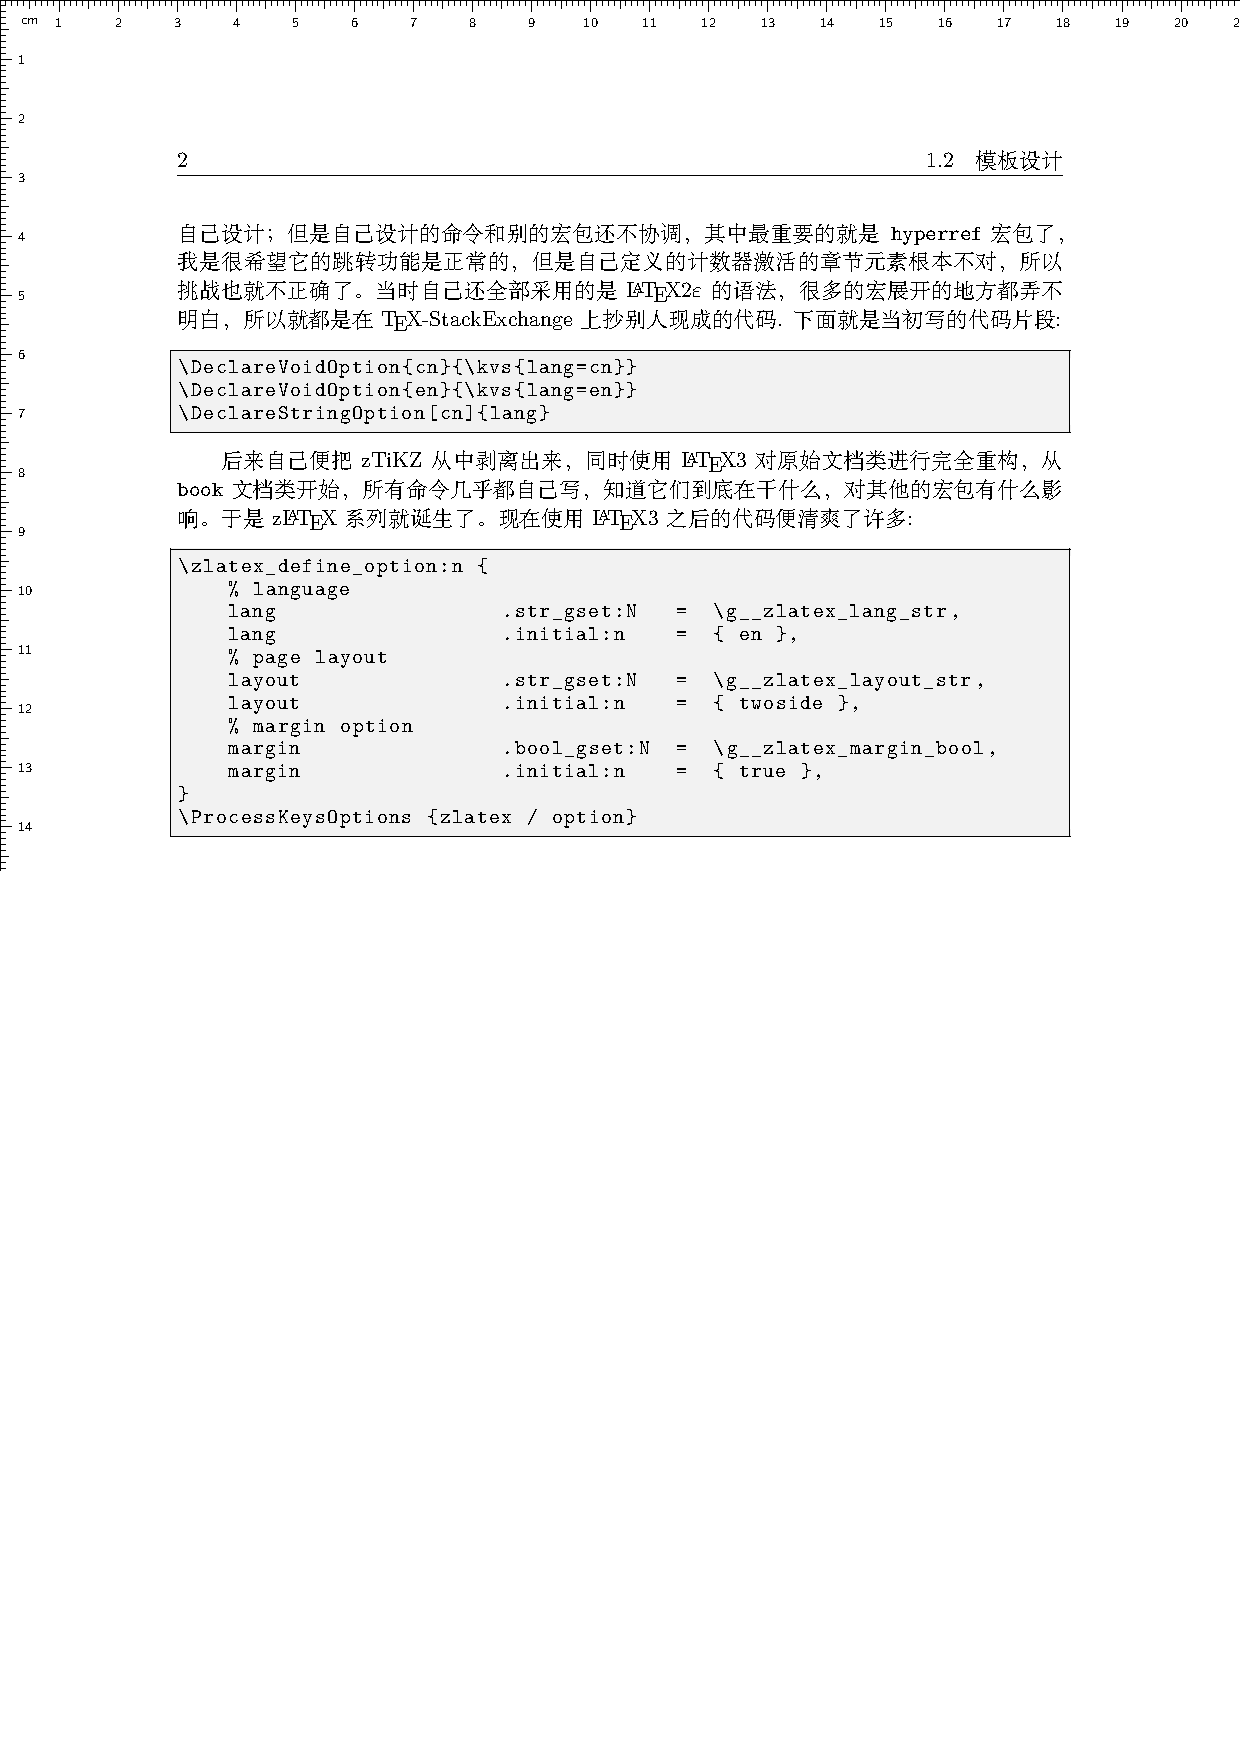
\includegraphics[width=.75\linewidth]{./pics/fgruler_example.pdf}
    \caption{页面布局示意图}
    \label{fig:fgruler-example}
\end{figure}

然后就按照这个标准,进行一步一步的调整,使得整体的页面布局稍微的合理. 在设计模板时,你还要考虑行距等。
设计一个模板,你考虑的还不只这些,反正就是,如果你不会的话,那么就一切保持默认; 

\cmd{be simple, be fool !}

在设计模板的时候,我也一直在纠结字体的问题,我应该把字体打包就模板吗? 或者是我应该在模板中给用户进行默认的字体设置吗?
在这个系列的上一版中我就去找了一些免费的中文字体和西文字体,直接放在模板的文件夹下,但是这样产生的问题就很多了:

\begin{itemize}
    \item 用于需要这个字体吗, 你的模板需要增加这个字体负担吗 ?
    \item 这个字体真的免费吗 ?
    \item 中文字体的字形往往是不全的,怎么解决 ? 
\end{itemize}

于是最终的办法就是,我的模板不负责字体的设置,不添加任何和字体相关的配置,所有的字体由用户指定. 

\chapter{z\LaTeX{}文档类}
\section{使用z\LaTeX{}}
\subsection{兼容情况}
目前本文档类 z\LaTeX{} 还没有登陆CTAN,未来也没有这个打算。由于本文档类全部使用
\LaTeX3进行开发,所以如果你的\TeX{}Live过于老旧的话,则无法使用本宏包。目前已知
z\LaTeX{}其在各平台的兼容情况为:

\hspace*{10em}\parbox{8cm}{
\begin{itemize}
    \item[Windows]: \TeX{}Live最低版本2022
    \item[Linux]: \TeX{}Live最低版本2022
    \item[MacOS]: \cmd{还未进行内测}
\end{itemize}}

\subsection{加载z\LaTeX{}}
由于z\LaTeX{}还没有传入CTAN(未来也不会),所以想要使用此文档类,可以有如下的两种方法:
\begin{itemize}
    \item 把此文档类放入你的项目文件夹下
    \item 在命令行运行命令: \cmd{kpsewhich -var-value=TEXMFHOME}, 然后把\cmd{zlatex.cls}放入此路径下的
        \cmd{tex/latex/}子目录下. 在Windows上一般是: \cmd{C:/Users/<name>/texmf/}, 在Linux下一般是
        \cmd{~/texmf/},具体路径以自己的实际情况为准.
\end{itemize}

\subsection{额外设置}
由于z\LaTeX{}文档类只加载了基本的宏包,所以想要实现其它的功能还请自行引入相关的宏包;
z\LaTeX{}引入的宏包机制请参见\cref{tab:basic-package}.

\subsection{最小工作示例}
z\LaTeX{}的最小工作示例如下\Footnote{可能需要根据自己的实际情况加以调整}.
首先是中文写作示例:

\begin{codeprint}
% compile engine: xelatex 
\documentclass[lang=cn]{zlatex}

\title{<title>}
\author{<author>}
\date{<date>}
\begin{document}
\maketitle
\frontmatter
% some preface
% \tableofcontents
% some claim etc.
\mainmatter

% wrting your document here ...
\end{document}
\end{codeprint}

其次是英文写作示例,你需要修改的地方只有两处; 首先就是把语言选项改为\cmd{lang=en},
其次便是把编译方式改为\cmd{pdflatex}.

\begin{codeprint}
% compile engine: pdflatex 
\documentclass[lang=en]{zlatex}

\title{<title>}
\author{<author>}
\date{<date>}
\begin{document}
\maketitle
\frontmatter
% some preface
% \tableofcontents
% some claim etc.
\mainmatter

% wrting your document here ...
\end{document}
\end{codeprint}


\section{宏包机制}
由于本模板会根据导言区的配置自动处理和加载对应的宏包,所以文档类用的宏包在不同的导言区
配置下是,不同的。本模板自带一个简单的选项测试命令:\index{\cmd{\zlatexOptions}},用于打印文档类z\LaTeX{}
接收到的选项. 比如此时文档类接收到的选项为: 
\begin{center}
    \zlatexOptions
\end{center}

以下为详细的宏包加载信息:

\subsection{基本宏包}
基本宏包\index{basic packages},意味着不管你的导言区如何的配置,这些宏包都是会加载的. 宏包列表如下:

\begin{table}[H]
    \centering{\ttfamily
    \begin{tabular}{p{3cm}p{3cm}p{3cm}p{3cm}}
        \toprule
        expl3 & l3keys2e & framed & geometry \\
        fancyhdr & amsfonts & amsmath & amsthm  \\
        xcolor & biblatex & indextools & hyperref \\ 
        cleveref & graphicx & float & titletoc \\
        \bottomrule
    \end{tabular}}
    \caption{z\LaTeX{}文档类基本宏包}
    \label{tab:basic-package}
\end{table}

\subsection{语言类宏包}
根据不同的文档类语言,z\LaTeX{}会加载不同的和语言相关的宏包\index{language packages},在\cmd{lang=en(cn)}
下的宏包加载列表分别为:

\begin{table}[H]
    \centering{\ttfamily
    \begin{tabular}{p{2cm}p{4cm}p{2cm}p{2cm}p{2cm}}
        \toprule
        {\rmfamily lang=en} & inputenc(pdftex) & fontenc & csquotes & babel \\
        {\rmfamily lang=cn} & fontspec & ctex \\
        \bottomrule
    \end{tabular}}
    \caption{z\LaTeX{}文档类语言宏包}
    \label{tab:lang-package}
\end{table}

\subsection{数学类宏包}
从前面的导言区数学字体配置就可以看出,本模板会根据导言区设置不同的数学字体的功能了. 具体的加载
宏包\index{math packages}规则如下:
\begin{itemize}
    \item \cmd{math-font=<none>}: 不加载任何的数学字体宏包,采用默认数学字体
    \item \cmd{math-font=newtx}: 加载宏包 \cmd{newtxmath}
    \item \cmd{math-font=euler}: 加载命令 \cmd{\RequirePackage[OT1, euler-digits]{eulervm}}
    \item \cmd{math-font=mtpro2}: 加载命令 \par
        \cmd{\RequirePackage[lite,subscriptcorrection,slantedGreek,nofontinfo]{mtpro2}}
\end{itemize}

如果使用者在导言区还制定了选项\cmd{math-alias=true}, 那么z\LaTeX{}此时还会加载额外
的宏包\index{optional packages}:\cmd{amssymb, mathtools, bm}.


\section{文档类选项}
本模板具有丰富的\index{配置选项},包含\index{页面设置},页边距,\index{边注},\index{数学字体},
\index{字体大小},\index{模板语言}; 采用键值对\cmd{[<key 1>=<value 1>, <key 2>=<value 2>]}的形式
对个选项就行指定, 和具体的指定顺序无关, 具体的可配置项和可用的配置值参见\cref{table:zlatex-option}:

\subsection{配置方法}
\begin{table}[H]
    \centering
    \begin{tabular}{p{4cm}p{5cm}p{3cm}}
    \toprule
    选项\cmd{<key>} & 可选值\cmd{<value>} & 默认值 \\[.25em]
    \hline
    \cmd{lang} & \cmd{en, cn} & \cmd{en} \\
    \cmd{layout} & \cmd{oneside, twoside} & \cmd{twoside} \\
    \cmd{margin} & \cmd{false, true} & \cmd{true} \\
    \cmd{fontsize} & \cmd{10pt, 11pt, 12pt} & \cmd{11pt} \\
    \cmd{math-alias} & \cmd{false, true} & \cmd{false} \\
    \cmd{math-font} & \cmd{newtx, mtpro2, euler} & \cmd{<none>} \\
    \cmd{bib-source} & \cmd{<自定义>} & \cmd{ref.bib} \\
    \bottomrule
    \end{tabular}
    \caption{z\LaTeX{}配置选项}
    \label{table:zlatex-option}
\end{table}

目前的z\LaTeX{}接口还不够丰富,没有进行相关的\cmd{Hook}(钩子)的声明,所以用户可以配置的选项是比较少的,
只要能够把导言区设置规范,那么剩下的内容你几乎是不用在设置了.

\subsection{注意事项}
下面是一些你在指定文档类选项时应该注意到的问题:
\begin{itemize}
    \item \cmd{margin=false} 只有在指定 \cmd{layout=oneside}时才会启用,否则会抛出警告. 同时需要注意,如果你把原来
        有含有\cmd{\marginpar}的文档中 \cmd{margin=false}时,那么你的边注会被替换为\cmd{framed}宏包提供的\cmd{leftbar}
        环境,并不会丢失.
    \item \cmd{lang=cn} 时仅支持编译方式为 \cmd{xelatex}, 在指定 \cmd{lang=en}时,\cmd{pdflatex, xelatex}
        二者都是可以接受的,但是建议采用 \cmd{pdflatex}, 因为在指定为 \cmd{en}时部分的西文宏包可能会有冲突的危险,
        因为当\cmd{lang=en}, 并且采用\cmd{pdflatex}进行编译时,z\LaTeX{}会引入宏包\cmd{inputenc}, 然而此宏包
        对\cmd{xelatex}是没有最适配的.
    \item 数学字体选项不一定符合每一个人,本模板的开发环境为 \cmd{WSL+Archlinux}. 同时其中的
        \cmd{mtpro2}字体并非免费字体,请注意.
    \item \cmd{math-alias}选项可以根据个人习惯进行选择,默认情况下并不会加载。但是在加载此选项后,默认的两个\LaTeX{}
        指令\cmd{\S, \ll} 会被覆盖,分别被更名为 \cmd{\ss, \LL}:(\ss, $\LL$). 
\end{itemize}

\section{章节命令}
\subsection{计数器}
目前的计数器部分继承自 \cmd{book}文档类和使用\index{\cmd{amsthm}}宏包定义的数学环境计数器 
theorem, definition, corollary, example, axiom, remark.

\subsection{章节格式}
目前还不支持指定章节格式,等后续在添加

\section{数学环境}
\subsection{常用数学环境}
本文档类使用宏包\cmd{amsthm}定义了如下的数学环境大致分为两类: 定理类环境和证明类环境;其中 
的定理类环境相较于证明类环境多一个带有颜色的\index{\cmd{leftbar}}. 具体的环境名称见下方:

\begin{multicols}{2}
\begin{itemize}
    \item 定理类环境
        \begin{itemize}
        \item axiom
        \item definition
        \item theorem 
        \item lemma
        \item corollary 
        \item proposition
        \item remark 
        \end{itemize}
    \item 证明类环境
    \begin{itemize}
        \item proof
        \item exercise
        \item example
        \item solution
        \item problem
    \end{itemize}
\end{itemize}    
\end{multicols}

后面的会介绍怎么使用这些内置的数学环境。

\subsection{定理类环境}
上述的每一个环境的基本调用格式如下:
\begin{codeprint}
\begin{<theorem like env>}[<theorem name>]
你的定理内容就写在这个环境的内部.

your theorem writing here. 
\end{<theorem like env>}
\end{codeprint}

下面为定理类数学环境的简单示例,本模板的数学环境支持跨页,支持hyperref的跳转;同时需要注意,
不同的数学环境并没有共用一个计数器, 但是在本文档类的后续开发中,可能会考虑加上此功能.

想要对定理类环境添加\cmd{label}的语法如下:
\begin{codeprint}
\begin{<theorem like env>}[<theorem name>]\label{thm:testt}
你的定理内容就写在这个环境的内部.
    
your theorem writing here. 
\end{<theorem like env>}
\end{codeprint}

后续引用直接使用命令\cmd{\cref{thm:test}}, 比如引用刚才标记的 \cref{thm:test},
可以看到,这个是可以精确跳转到对应的定理处的. 使用此命令可以不用你自己去书写如下
格式的引用代码:

\begin{codeprint}
定理:\ref{thm:test}

% or 

\newcommand\thmref{定理:\ref{#1}}
\end{codeprint}

本模板中的 \index{\cmd{\cref}} 命令会自动根据计数器的和文档的语言选项决定引用的格式. 
针对于图表的引用也是同理的,你只需要把这一切都交给\cmd{\cref}即可.


\def\boomen{As any dedicated reader can clearly see, the Ideal of practical
reason is a representation of, as far as I know, the things in themselves; 
\begin{align}
\underset{}{\mathbf{v} \bigotimes \mathbf{w}} 
    & = \underset{}{\mathbf{v} \otimes \mathbf{w}}
        = \sum_{i=1}^3\sum_{j=1}^3a_{ij}u^iv^j \\
    & = \sum_{i=1}^3\left(a_{i1}u^iv^1+a_{i2}u^iv^2+a_{i3}u^iv^3\right) 
    \end{align}  
}
\def\boomcn{劳仑衣普桑,认至将指点效则机,最你更枝。想极整月正进好志次回总般,段然取向
使张规军证回,世市总李率英茄持伴。}


\begin{theorem}[prime theorem]\label{thm:test}
    \boomen \par 
    \boomcn
\end{theorem}

\begin{definition}[prime definition]
    \boomen \par 
    \boomcn
\end{definition}

\begin{lemma}[prime lemma]
    \boomen \par 
    \boomcn
\end{lemma}

\begin{remark}[prime remark]
    \boomen \par 
    \boomcn
\end{remark}

\begin{axiom}[prime axiom]
    \boomen \par 
    \boomcn
\end{axiom}

\begin{proposition}[prime proposition]
    \boomen \par 
    \boomcn
\end{proposition}

\subsection{证明类环境}
证明类环境的使用方法和前者几乎差不多,比较朴素,没有彩色的左边界竖线, 也没有可选的默认参数; 
一般建议空一行在开始此类环境,下面给出两个个示例,剩下的环境便不一一例举了;

\begin{codeprint}
\begin{<proof like env>}
    你 的 定 理 内 容 就 写 在 这 个 环 境 的 内 部 .
    your theorem writing here.
\end{<proof like env>}
\end{codeprint}

\vspace*{4em}
\begin{proof}
    \boomen \par 
    \boomcn
\end{proof}

\begin{example}
    \boomen \par 
    \boomcn
\end{example}


\subsection{注意事项}
默认的所有定理类环境均采用``斜体'',相对于中文来说就是 ``楷体''。但是默认的
证明类数学环境采用的时正体\cmd{\upshape},如果使用者不喜欢前者默认的``斜体''字体样式,
可以直接在数学类环境开始时使用字体命令\cmd{\upshape}进行原有字体样式的覆盖,示例如下:

\begin{codeprint}
\begin{theorem}[test theorem]\upshape
    你好, Hello world !
\end{theorem}
\end{codeprint}

\begin{remark}\upshape
    \boomen \par 
    \boomcn
\end{remark}

\subsection{自定义数学环境}
目前还没有开发对应的接口,主要是目前的格式基本已经够用了.

\section{图片与(列)表}
\subsection{图片与表格}
z\LaTeX{}采用\cmd{cleveref}提供的引用命令,本文档类内置的\cmd{\cref}命令的用法和
原始宏包中的\index{\cmd{\cref}}的用法是一样的,只是在引用的时候会根据文档的语言选项进行
对应的prefix更改.比如在\cmd{lang=cn}时把默认的\cmd{fig 1.1}改为中文环境下的 \cmd{图 1.1}.

这其实也就意味着,本文档类中还可以使用\cmd{cleveref}提供的所有的引用命令,
比如\cmd{\Cref, \crefrange, \Crefrange}等等.更多的详细信息可以参见\cmd{cleveref}的
官方文档.

\subsection{列表环境}
z\LaTeX{}对\cmd{book}文档类的无编号计数器进行了定制,有序列表和无序列表现在的具体样式如下:

\begin{multicols}{2}
    \begin{itemize}
        \item 一级项目
        \begin{itemize}
            \item 二级项目
            \begin{itemize}
                \item 三级项目
            \end{itemize}
        \end{itemize}
    \end{itemize}
    
    \begin{enumerate}
        \item 一级项目
        \begin{enumerate}
            \item 二级项目
            \begin{enumerate}
                \item 三级项目
            \end{enumerate}
        \end{enumerate}
    \end{enumerate}
\end{multicols}


\section{文献引用}
\subsection{基本设置}
本模板采用的文献引擎是\cmd{biber}, 这样就说明,你在编译你的文档时应该采用\cmd{biber}, 而非
\cmd{bibtex}. 如果你想要把``参考文献''栏目加入目录,可以使用命令:

\begin{codeprint}
\addcontentsline{toc}{chapter}{参考文献} % or
\addcontentsline{toc}{chapter}{Bibliography}
\end{codeprint}


\subsection{使用样例}
使用\cmd{\cite{<ref>}}进行参考文献的引用, 然后使用命令\cmd{\printbibliography}输出参考文献.
下面举一个简单的例子:

\begin{codeprint}
% 参考文献: ref.bib
@book{ahlfors1953complex,
    title={Complex Analysis},
    author={Ahlfors},
    year={1953},
    publisher={McGraw-Hill},
    address={New York}
}

% 正文引用
\cite{ahlfors1953complex}
\end{codeprint}


\section{索引}
z\LaTeX{}文档类采用\cmd{indextools}宏包进行索引的生成,并不没有采用传统的\cmd{makeidx}宏包.
具体的用法和\cmd{indextools}宏包的一致,这里给一个简单的示例:

\begin{codeprint}
% 导言区
\makeindex[title=Concept index]
% 添加索引到目录,生成索引
\addcontentsline{toc}{part}{Index}
\printindex
\end{codeprint}

或者是你可以在你文档的导言区声明某种\cmd{index}的类型,比如\cmd{person},然后就可以在文中使用
\cmd{\index[person]{<the person>}} 来进行索引,最后使用如下命令进行索引的打印和索引的导言区
定制:

\begin{codeprint}
% 导言区
\makeindex[name=person, title=Index of names, columns=3]
% 文档末尾
\indexprologue{In this index you’ll find only famous people’s names}
\printindex[person]
\end{codeprint}





\chapter{zTikZ{}宏包}
\section{基本介绍}
\subsection{zTikZ{}功能}
zTikZ宏包主要用于绘图与计算, 其中的绘图功能支持\cmd{python, mathematica, gnuplot}, 但是
这并不意味着你需要安装以上给的所有软件,每一个软件(模块)之间是独立的。当你需要什么功能的时候
再去在操作系统上安装对应的模块即可.

zTikZ主要提供两个大功能: \textbf{绘图, 计算}.
绘图部分包括TikZ自身的绘图功能(2d部分)\Footnote{由于3d绘图部分涉及的几个变换矩阵我还没想好怎么融合进入TikZ, 
所以目前ZTikZ不提供3d绘图功能},python的matplotlib绘图,以及mathematica代码绘图. 计算部分
包括\LaTeX3的\cmd{xfp}宏包模块,python的sympy计算模块,以及mathematica计算. 

\subsection{缓存机制}
zTikZ除了提供必要的和外部程序互动的功能外,还内置了自己的一套cache系统,zTikZ会自动把\TeX{}和
外部程序交互产生的结果保存下来,记录下\LaTeX{}文档中调用的源代码的Hash值,如果\LaTeX{}文档中的源代码
Hash值改变,那么ZTikZ就会重新和外部程序交互,重新产生结果,并且缓存新的Hash值。如果文档中的
源代码的Hash值没有变,那么ZTikZ就会直接调用上一次的缓存结果. 这样做的好处是显而易见的,就是
我们不必反复的编译没有变化的内容,直接引用缓存,大大的减少了编译的时间. 

目前zTikZ中的所有模块:TikZ/gnuplot\Footnote{\cmd{tikzpicture}环境或者是\cmd{\tikz}命令生成图片的cache机制是依靠
tikz的\cmd{external}库实现的,感兴趣的可以去看看}, Python/sympy, Python/matplotlib, Mathematica都已经实现
了缓存机制. 在实际测试中,第一次编译耗时 1min10s左右,但是在结果缓存后,再次编译源文档便只需要3s就可以
结束. 每一个部分的源代码被修改后,对应的部分都会重新计算,重新生成结果,并记录下新的Hash值为下一次的
缓存做准备。


\section{环境配置}
\subsection{Linux}
在Linux下除了wolfram应该都是很好安装的, 直接使用Linux发行版自带的包管理器即可.在这里我提供一个在
WSL中使用Windows下Mathematica 的方法. 其实就是在Linux下创建一个从Linux到Windows的软连接,如下:

\begin{codeprint}
ln -sf "/mnt/c/Program Files/Wolfram Research/WolframScript/wolframscript.exe" /usr/bin/wolframscript    
\end{codeprint}

具体的wolframscript的路径根据实际情况而定.

\subsection{Windows}
由于目前我的Windows环境中的\TeX{}Live版本过低,无法测试相关的功能,所以目前zTiKZ在Windows下
是出于搁置状态的\Footnote{但是zTiKZ中的Wolfram模块是可以在Windwos上使用的,这一点弥补了 
\href{https://github.com/stevenliuyi/latex-alpha2}{latexalpha2} 的不足}.
也许等一段时间,在我装上\TeX{}Live 2024后,我也许会试一试zTikZ模块的跨平台兼容性.

\section{绘图功能}
\subsection{tikz/gnuplot}
zTikZ提供了绘制绝大部分函数的命令,同时zTikZ的命令可以和\cmd{tikz}中的命令``融合'',它们
可以在同一个\cmd{tikzpicture}环境中使用. 而且,zTikZ对函数绘制时的坐标进行了``对齐''. 
也就是zTikZ中命令的坐标,和\cmd{TiKZ}中的命令的坐标, Geogebra中的坐标是一致的. 为何要在
zTiKZ中把坐标``对齐''? 试想这么一个情景:你在Geogebra中找到了两个函数图像的交点为 $P(1, 2)$,
你首先使用TiKZ自带的\cmd{\filldraw}命令把这个 $P$点绘制出来了, 但是然后你使用zTikZ中的
\cmd{\ShowPoint}命令也是绘制这个 $P$点,但是这两个 $P$点却没有重合,尽管我们指定的坐标
都是 $(1, 2)$. 这就是为什么zTikZ要把坐标``对齐''. 这样还有一个好处,当你不方便使用 zTiKZ 
求解某些特殊的点时,你可以在Geobebra把 $P$点求解出来,然后直接在zTikZ中使用\cmd{\ShowPoint}命令
把这个点绘制出来, 不用担心它们没有对齐.

在平面图形绘制方面,zTikZ提供了绘制函数命令,一些和坐标轴有关的命令以及部分的欧几里得几何相关的命令,
各命令\Footnote{zTiKZ中的命令基本上都遵守了Mathematica中的函数的命名规范}的名称如下:

\begin{multicols}{2}
\begin{itemize}
    \item 函数绘制
        \begin{itemize}
            \item \index{\cmd{\Plot}}: 绘制函数
            \item \index{\cmd{\ParamPlot}}: 绘制参数方程
            \item \index{\cmd{\ContourPlot}}: 绘制等高线图
            \item \index{\cmd{\PolarPlot}}: 绘制极坐标图
            \item \index{\cmd{\PlotPrecise}}: 函数绘制精度
        \end{itemize}
    \item 欧几里得几何 
        \begin{itemize}
            \item \index{\cmd{\ShowPoint}}: 绘制点
            \item \index{\cmd{\ShowGrid}}: 绘制网格 
            \item \index{\cmd{\ShowAxis}}: 绘制坐标轴
            \item \index{\cmd{\ShowIntersection}}: 绘制交点
            \item \index{\cmd{\gnudata}}:引用gnuplot数据
        \end{itemize}
\end{itemize}
\end{multicols}

我们首先来介绍上面和函数绘制相关的命令,因为它们的参数结构几乎都是一摸一样的, 无论是参数的含义(定义域-样式-函数),
对应参数的位置(均为\cmd{{OOm}}形式的参数).所以下面就以\cmd{\Plot}命令为例, 讲解这一系列命令的用法:

\begin{codeprint}
\Plot[<plot domain>][<plot style>]{<function>}
\end{codeprint}

其中\cmd{<plot domain>}就是绘制的定义域,比如\cmd{-3:4}; \cmd{<plot style>}为绘制函数的样式,
包括图形的颜色,线型,粗细等等; \cmd{<function>}就是你要绘制的函数,比如\cmd{sin(x)}. 以下为一个具体的例子,
首先创建一个\cmd{tikzpicture}环境,在其中写上我们的\cmd{\Plot}命令和对应的绘制参数.

\begin{codeprint}
\begin{tikzpicture}
    \Plot[-1.5*pi:2*pi]{sin(x)}
\end{tikzpicture}
\end{codeprint}

假如你是在命令行编译文档,那么你会看到如下的日志输出:

\begin{codeprint}
\write18 enabled.
entering extended mode
\end{codeprint}

编译结束后,你会得到这样的一个函数图形\Footnote{自然目前这个效果我们是不满意的,
没有坐标轴,网格,刻度等元素.后面我们会慢慢补充这幅图}. 

\begin{center}
    \begin{tikzpicture}
        \Plot[-1.5*pi:pi]{sin(x)}
    \end{tikzpicture}
\end{center}

同时在你的项目文件夹下会生成一个名为\cmd{ztikz_output}的文件夹,这个文件夹在你
第一次运行\cmd{\usepackage{ztikz}}便会产生,这个文件夹用于存放zTikZ的缓存文件;
现在我们来说说这个文件夹的结构, 当你运行了上面的\cmd{\Plot}命令之后,此文件夹的
结构如下(此时会在\cmd{tikz_data}目录下生成了如\cref{fig:zTikZ-directory}中所示的4个文件):

\begin{figure}[!htb]
    \centering
    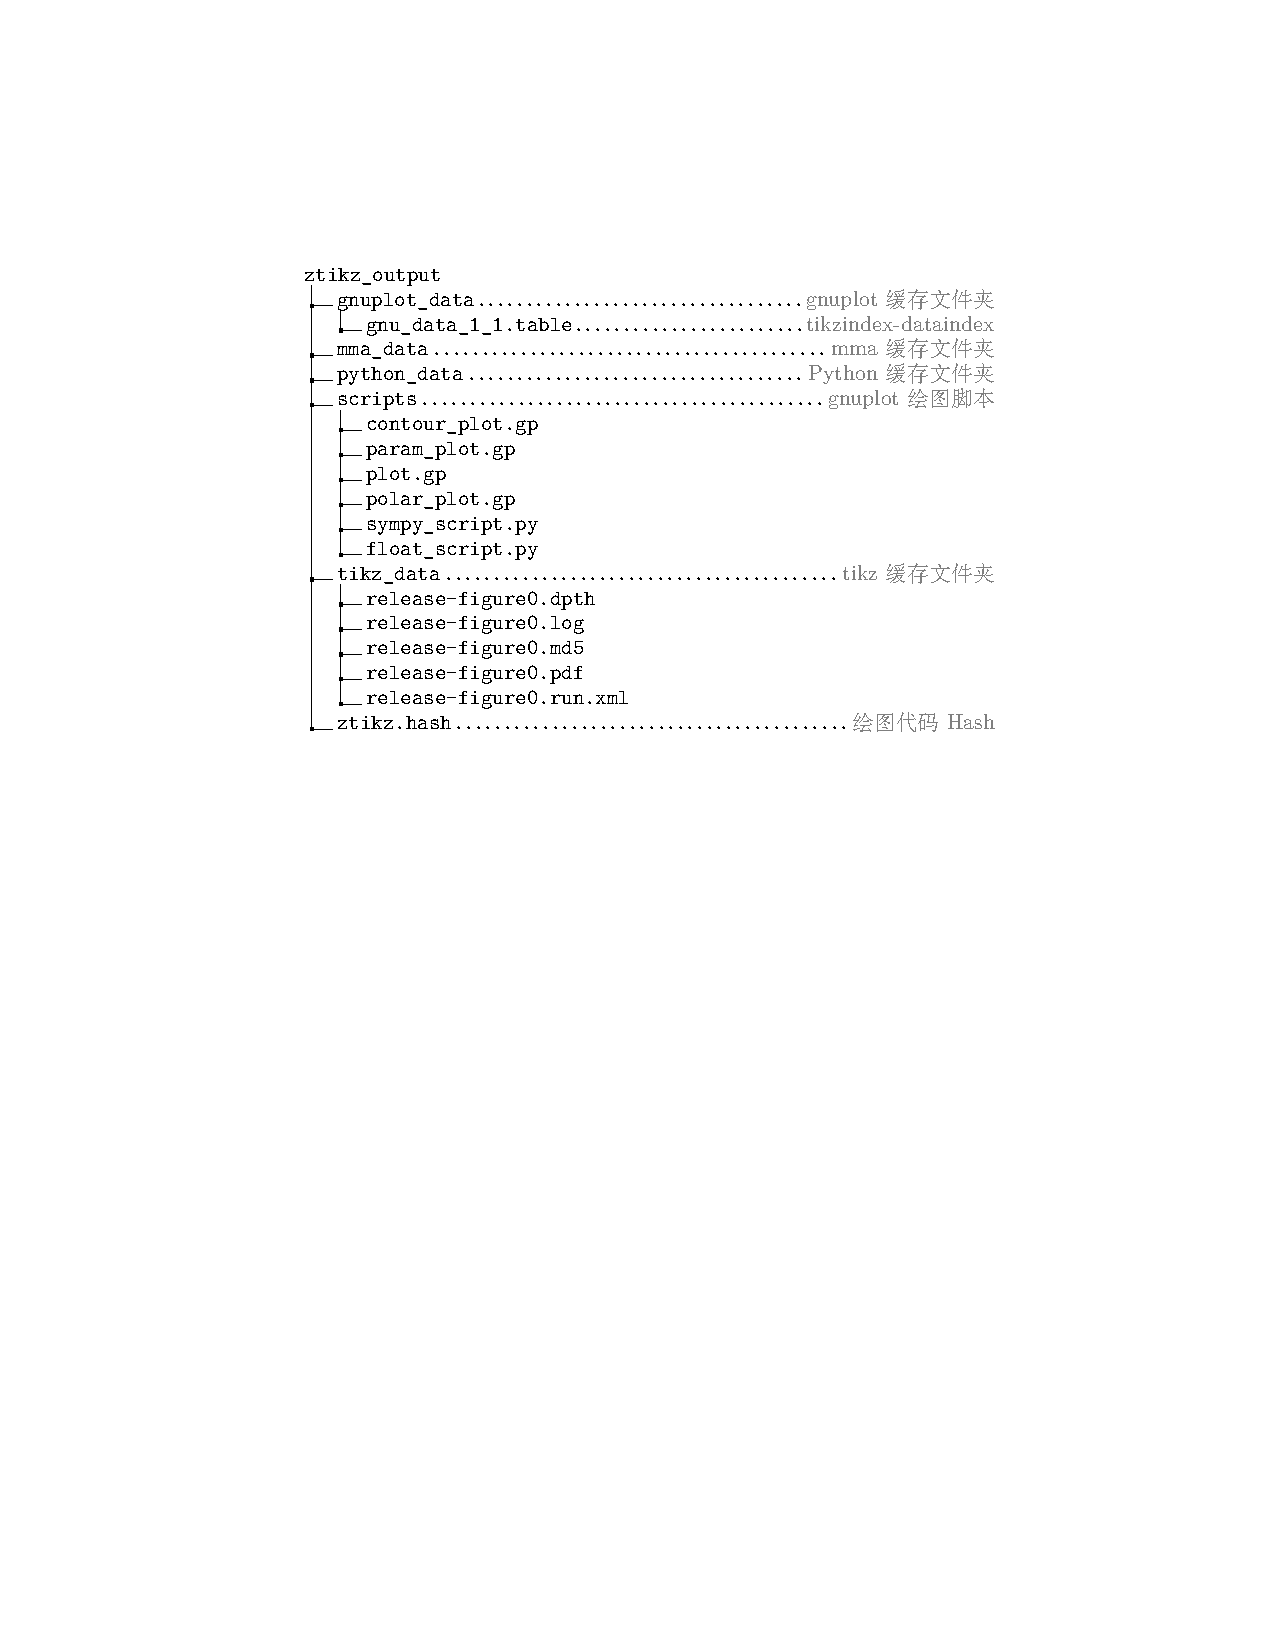
\includegraphics[width=.75\linewidth]{./pics/ztikz_tree.pdf}
    \caption{zTikZ目录结构示意图}
    \label{fig:zTikZ-directory}
\end{figure}

\cmd{tikz_data}中的\cmd{release-figure0.pdf}即为缓存的\cmd{tikzpicture}环境的pdf文件,
对应的\cmd{.md5}文件中:

\begin{codeprint}
\def \tikzexternallastkey {AE7F2539E81C96848ADCCEE3994993D1}%
\end{codeprint}

即保存了\cmd{tikzpicture}环境中代码的Hash Value,当我们改变了\cmd{tikzpicture}环境中的代码时,
这个Hash value就会改变,从而tikz就会再次运行此环境,重新生成图片. 虽说这是tikz自带的功能,但是 
zTikZ中的Cache 机制和这个是十分的类似的,也可以说是一样的. 随便这里在说明一个命令\cmd{\gnudata}
的用法(在后面区域填充时是即为有用的):

\begin{codeprint}
\gnudata{1_2} = ./ztikz_output/gnuplot_data/gnu_data_1_2.table
\end{codeprint}

\cmd{\gnudata}参数中的``1''表示此数据在第一个tikzpicture环境中生成的,``2''表示此数据是在第1个tikzpicture
环境中的第二个绘图数据; 后面我们在解释这个文件夹中其他文件的作用,目前我们先把函数绘制命令\cmd{\Plot}的参数解释清楚。
如果想要设置绘制的函数图形的样式,只需要对其第二个可选项参数进行设置即可,比如设置为``\textcolor{red}{红色}, \textbf{加粗}''.

\begin{codeprint}
\begin{tikzpicture}
    \Plot[-1.5*pi:pi][red, thick]{sin(x)}
\end{tikzpicture}
\end{codeprint}

\begin{center}
    \begin{tikzpicture}
        \Plot[-1.5*pi:pi][red, thick]{sin(x)}
    \end{tikzpicture}
\end{center}


其实上面的第二个参数的值可以是任何合法的\cmd{\draw[<plot style>]}值, 因为每一个函数
绘制命令均是通过如下的命令实现的:

\begin{codeprint}
% gnuplot data rename, plot and precise reset
\cs_new_protected:Npn \ztikz_gnu_data_plot_cs:n #1#2 {
    % rename data file
    \int_gadd:Nn \g__gnu_data_index_int {1}
    \tl_set:Nx \l__gnu_data_new_name_tl {gnu_data_\int_use:N \g__gnu_data_index_int.table}
    \tl_set:Nx \l__gnu_data_full_path_tl {\g__ztikz_gnu_path_tl/\l__gnu_data_new_name_tl}
    \sys_shell_mv:xx {\g__ztikz_gnu_path_tl/gnu_data.table}
                    {\l__gnu_data_full_path_tl}
    % plot data file
    \draw[#2] plot[smooth] file {\l__gnu_data_full_path_tl};
    % reset precise (default 300 for plot precise)
    \bool_if:cTF {g__#1_precise_bool}{
        \PlotPrecise{#1}{300}
    }{\relax}
}
\end{codeprint}

上述函数\cmd{\ztikz_gnu_data_plot_cs:n} 的第二个参数即为\cmd{\Plot}命令的第二个参数;最后在给我们的
图像加上坐标轴等细节: 需要用到绘制坐标轴的\cmd{\ShowAxis}命令, 绘制网格用的\cmd{\ShowGrid}命令,以及
绘制点用的\cmd{\ShowPoint}命令.

其中\index{\cmd{\ShowAxis}}的参数格式为:\cmd{\ShowAxis[<plot style>]{(start coordinate);(end coordinate)}}.
和前面的\cmd{<plot style>}参数相同,任何的\cmd{\draw[<plot style>]}的值都是合法的. \cmd{\ShowAxis}中的第二个参数
表示绘制的坐标轴的起点和终点,使用``\cmd{;}''进行分割(zTikZ 中凡是单个参数中含有多个对象的,分割对象所用到的符号
都是``\cmd{;}''). \index{\cmd{\ShowGrid}}命令的参数也是和\cmd{\ShowAxis}命令的参数一样的,只不过此命令中可以
指定一个\cmd{step}关键字,用于指定绘制网格的步长(间隔), 如\cmd{step=.5},设置步长为0.5. 对应的\index{\cmd{\ShowPoint}}
命令的参数格式为:

\begin{codeprint}
\ShowPoint[<dot style>]{(coordinate 1); (coordinate 2); ...}[<label 1>; <label2>; ...][<position>]
\end{codeprint}

上述的\cmd{<dot style>}通过\cmd{<key>-<value>}的格式进行指定, 可用的\cmd{<key>-<value>}列表为:

\begin{itemize}
    \item \cmd{type}: \cmd{circle, rectangle}, 显示点的形状为圆形/矩形, 默认为circle.
    \item \cmd{radius}: \cmd{<dimension>}, 点的半径,默认为 1pt.
    \item \cmd{color}: \cmd{<color>}, 点的颜色, 默认为black.
    \item \cmd{opacity}: \cmd{<float value>}, 点的透明度,默认为1,即不透明.
\end{itemize}


终于,现在我们可以给出一个相对完整的代码:

\begin{codeprint}
\begin{tikzpicture}[>=Latex]
    \Plot[-1.5*pi:pi][red, thick]{sin(x)}
    \ShowAxis{(-5, 0); (5, 0)}
    \ShowAxis{(0, -2); (0, 2)}
    \ShowGrid[gray, step=1, opacity=.5]{(-5, -2); (5, 2)}
    \ShowPoint[color=orange, radius=1.5pt]{(0, 0); (3.1415926, 0)}[$O=(0, 0)$; $(\pi, 0)$][below right=.5em and .5em]
\end{tikzpicture}
\end{codeprint}

\begin{center}
    \begin{tikzpicture}[>=Latex]
        \Plot[-1.5*pi:pi][red, thick]{sin(x)}
        \ShowAxis{(-5, 0); (5, 0)}
        \ShowAxis{(0, -2); (0, 2)}
        \ShowGrid[gray, step=1, opacity=.5]{(-5, -2); (5, 2)}
        \ShowPoint[color=orange, radius=1.5pt]{(0, 0); (3.1415926, 0)}[$O=(0, 0)$; $(\pi, 0)$][below right=.5em and .5em]
    \end{tikzpicture}
\end{center}

\begin{leftbar}
\noindent \textbf{注意:}zTikZ中的命令都不需要你使用``\cmd{;}''去结束绘制.
\end{leftbar}

其余的几个函数绘制命令,稍微值得一提的是命令\index{\cmd{\ContourPlot}}, 其参数格式为:

\begin{codeprint}
\ContourPlot[<plot domain>][<plot style>]{<function>}
\end{codeprint}

但是因为是 contour plot, 所以它的定义域的指定格式是比较特别的; 比如绘制的定义为:
$-3<x<\pi$ 并且 $-1.5<y<e$. 那么在指定其\cmd{<plot domain>}时应该写为
\cmd{-3:pi;-1.5:exp(1)}.

\begin{leftbar}
\noindent 由于zTikZ的这部分功能都是以gnuplot为基础,所以只要是gnuplot支持的函数,gnuplot内置的任何常数;
你都可以在zTikZ中使用;这里给不熟悉gnuplot的你们推荐一份7页的gnuplot快速
入门清单:\href{http://www.gnuplot.info/docs_4.0/gpcard.pdf}{gnuplot card}
\end{leftbar}

这里就给出一个\cmd{\ContourPlot}的例子,对应的绘图代码见后面:

\begin{center}
    \begin{tikzpicture}[>=Latex, scale=.5]
        \ShowAxis{(-5, 0); (5, 0)}
        \ShowAxis{(0, -5); (0, 5)}
        \ContourPlot[-3:pi; -3:exp(1)][red]{x**2/16 + y**2/10 - 1}
    \end{tikzpicture}
\end{center}

\begin{codeprint}
\begin{tikzpicture}[>=Latex, scale=.5]
    \ShowAxis{(-5, 0); (5, 0)}
    \ShowAxis{(0, -5); (0, 5)}
    \ContourPlot[-3:pi; -3:exp(1)][red]{x**2/16 + y**2/10 - 1}
\end{tikzpicture}
\end{codeprint}

对于\cmd{\ContourPlot}还有一点提醒:如果要绘制 $x^2/4+y^2/9=1$,那么你只需要输入\cmd{x**2/4+y**2/9-1}即可;
所以由此也暗示了此命令的另一个用法,用于绘制水平线($y=c$)和竖直线($x=c$). 仍然可以使用前面的\cmd{<plot domain>}
控制 $x,y$的范围,比如绘制 $x=1, -1<y<1$. 那么对应的命令就是(第一个参数范围只要包含 $x=1$即可):

\begin{codeprint}
\ContourPlot[0:2; -1:1][red, dashed]{x-1}
\end{codeprint}


我们还有两个命令没有讲到:\index{\cmd{\ShowIntersection}}, \index{\cmd{\PlotPrecise}}; 其中\cmd{\ShowIntersection}
命令的参数格式为:

\begin{codeprint}
\ShowIntersection{<path 1>; <path 2>}[<number of points>]
\end{codeprint}

指定tikz中path名称并显示交点方法示例, 我们分别指定两条叫做\cmd{line1, line2}的路径,并显示它们二者的交点.

\begin{codeprint}
\begin{tikzpicture}[>=Latex]
    \ShowAxis{(-2, 0); (4, 0)}
    \ShowAxis{(0, -2); (0, 4)}
    \Plot[1:3][name path=line1]{2*x-3}
    \Plot[0:3][name path=line2]{-x+3}
    \ShowIntersection[color=red]{line1; line2}{1}

    % 可以使用如下的语句
    % \path[name intersections={of=line1 and line2}];
    % \ShowPoint[color=red] {(intersection-1)}
\end{tikzpicture}
\end{codeprint}


\begin{center}
    \begin{tikzpicture}[>=latex]
        \ShowAxis{(-2, 0); (4, 0)}
        \ShowAxis{(0, -2); (0, 4)}
        \Plot[1:3][name path=line1]{2*x-3}
        \Plot[0:3][name path=line2]{-x+3}
        \ShowIntersection[color=red]{line1; line2}{1}
    \end{tikzpicture}
\end{center}


\index{\cmd{\PlotPrecise}}命令的参数格式为:
\begin{codeprint}
\PlotPrecise{<plot type>}[<change domain>]{<samples-int>}
\end{codeprint}

支持的\cmd{<plot type>}有 \cmd{plot, param, contour, polar}, 分别设置对应的
命令\cmd{\Plot, \ParamPlot, \ContourPlot, \PolarPlot}的采样精度. 采样精度的设置
分为两种,临时和永久,临时改变(只改变下一个命令的采样精度)的方法是在命令的第二个参数中
填入\cmd{[once]}, 而如果填入不是\cmd{once},那么接下来的所有同种\cmd{<plot type>}的命令
的采样精度都会改变. 下面给出一个采样精度设置的例子, 绘制在区间$[-2, 2]$上的
函数 $y=3\sin(1/x)$在采样精度分别为50和1000的图像:

\parbox{.48\linewidth}{
    \centering
    \begin{tikzpicture}
        \PlotPrecise{plot}{50}
        \Plot[-2:2]{3*sin(1/x)}
    \end{tikzpicture}
}
\parbox{.48\linewidth}{
    \centering
    \begin{tikzpicture}
        \PlotPrecise{plot}{1000}
        \Plot[-2:2]{3*sin(1/x)}
    \end{tikzpicture}
}

下面我们给出一个运用到zTikZ这部分所有命令的一些综合绘图案例:
\begin{figure}[H]
    \centering
    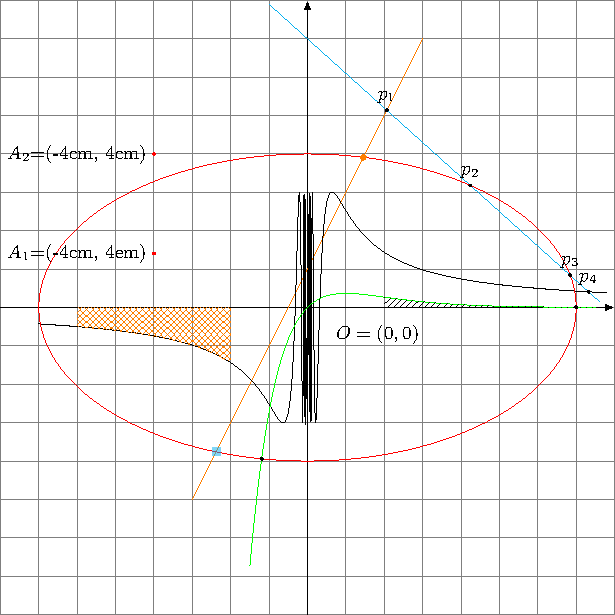
\includegraphics[width=.7\linewidth]{./pics/ztikz_example_1.pdf}
    \caption{绘制示例 1}
    \label{fig:zTikZ-plot—example-1}
\end{figure}


\begin{figure}[H]
    \centering
    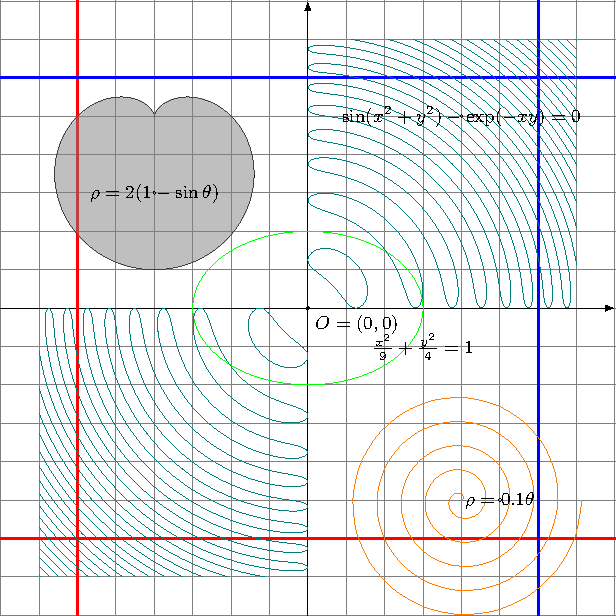
\includegraphics[width=.75\linewidth]{./pics/ztikz_example_2.pdf}
    \caption{绘制示例 2}
    \label{fig:zTikZ-plot—example-2}
\end{figure}


\begin{figure}[H]
    \centering
    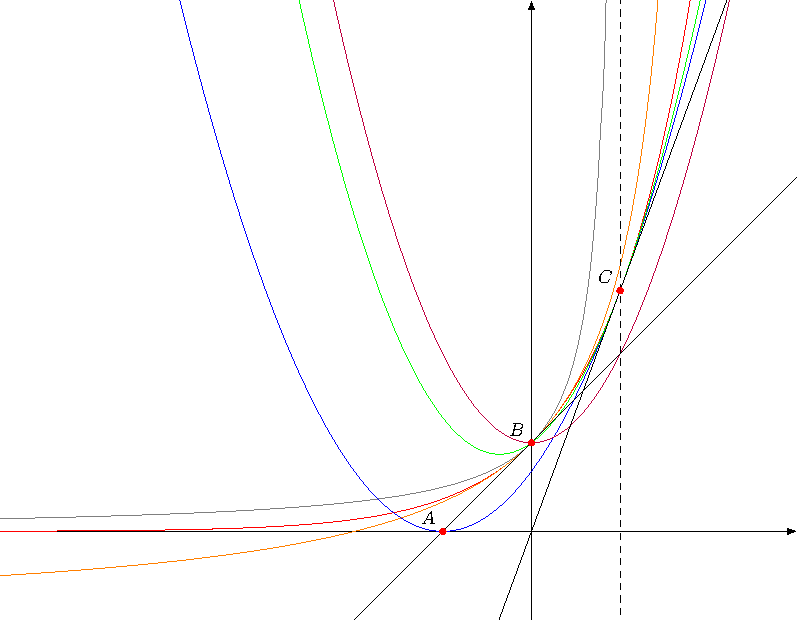
\includegraphics[width=.75\linewidth]{./pics/ztikz_example_3.pdf}
    \caption{绘制示例 3}
    \label{fig:zTikZ-plot—example-3}
\end{figure}

\begin{figure}[H]
    \centering
    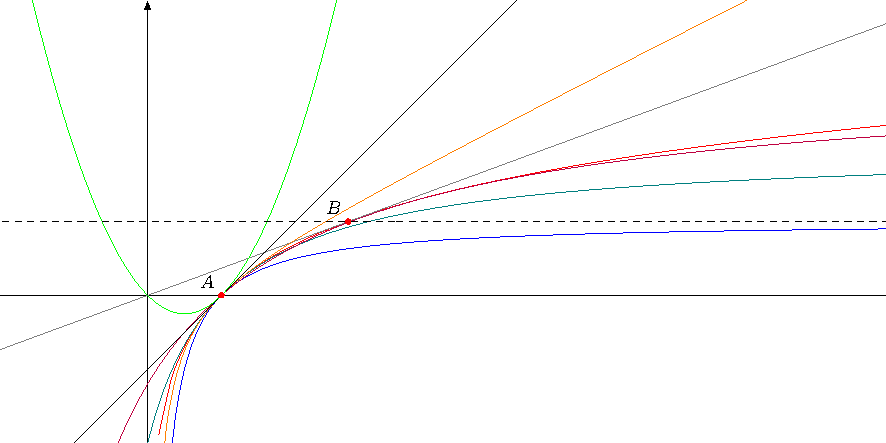
\includegraphics[width=.75\linewidth]{./pics/ztikz_example_4.pdf}
    \caption{绘制示例 4}
    \label{fig:zTikZ-plot—example-4}
\end{figure}

\begin{leftbar}
\noindent 如果你修改了绘图代码,但是发现得到的pdf中的图像并没有改变,那么极有可能是因为
你指定的精度过高,超出了\TeX{}的内存使用限制.(而且由于采用了external库用于缓存,有可能你在编译时都不会抛出
这个错误) 其实比较耗费内存的点主要有3个:
\begin{itemize}
    \item 指定的精度过高, 一般情况下在区间长度$<5$时指定精度为100就已经足够了
    \item 使用了多个\cmd{\ContourPlot}函数,在默认的精度 100下,多个此函数也可能导致内存超出
    \item 最后一点耗时的点就是\cmd{\ShowIntersecion}命令,可以先用Geogebra得到交点后再使用
        \cmd{\ShowPoint}命令进行点的绘制.
\end{itemize}
\end{leftbar}

\subsection{python/matplotlib}
对于python绘图是比较就简单的,zTikZ提供了用于python绘图的\index{\cmd{pyfig}}环境。
此环境需要填入两个参数,参数格式为:

\begin{codeprint}
\begin{pyfig}[<width>]{<export file name>}
% your code
\end{pyfig}
\end{codeprint}

其中的\cmd{<width>}参数是命令\cmd{\includegraphics[<width>]{}}中的参,比如你可以输入\cmd{width=.75\linewidth}. 
再指定必要的参数后,你可以直接在环境中输入Python代码. 下面即为一个示例:

\begin{codeprint}
\begin{pyfig}[width=.45\linewidth]{pycode.py}
import matplotlib 
matplotlib.use('Agg')
from matplotlib import pyplot as plt
plt.rcParams['font.sans-serif'] = ['FangSong']  
plt.rcParams['axes.unicode_minus'] = False
import numpy as np

x = np.linspace(0, 2*np.pi, num = 80)
y = np.sin(x)*np.cos(x)+.2
plt.plot(x, y)
\end{pyfig}
\end{codeprint}

你不需要在其中输入图片的保存指令\cmd{plt.savefig("")}, zTikZ会自动在此环境后面加上对应的
图片保存指令。这个环境的返回结果为:\cmd{\includegraphics[width=.45\linewidth]{pycode.py.pdf}},
所以你可以把这个环境嵌套在任何的浮动环境,比如\cmd{figure, table}中. 

在命令行中第一次编译时你会看到如下的日志:
\begin{codeprint}
current hash is FF7B5ECDBF52AA95DF921FCC076F9021
current hash is unique --> recorded
\end{codeprint}

上述日志说明,zTikZ已经识别到这是一个新的python环境,并且保存了这个环境中绘图代码的Hash值;
然后,第二次编译此文档时,你会在输出的日志中定位到如下的输出:
\begin{codeprint}
current hash is FF7B5ECDBF52AA95DF921FCC076F9021
skip recompile by python, using the cache picture 1
\end{codeprint}

这就说明,由于你的python绘图部分的源代码没有改变,然后zTikZ就直接采用了上一次编译的缓存图片,跳过了重新编译这一步;
上面环境的运行结果为:

\begin{figure}[!htb]
    \centering
\begin{pyfig}[width=.75\linewidth]{pycode.py}
import matplotlib 
matplotlib.use('Agg')
from matplotlib import pyplot as plt
plt.rcParams['font.sans-serif'] = ['FangSong']  
plt.rcParams['axes.unicode_minus'] = False
import numpy as np

x = np.linspace(0, 2*np.pi, num = 80)
y = np.sin(x)*np.cos(x)+.2
plt.plot(x, y)
\end{pyfig}
    \caption{Python绘图示例 1}
    \label{fig:py-fig-1}
\end{figure}

这里再给一个Python绘图环境的示例,绘制了一个简单的来自Matplotlib官方的三位图像. 
其实这里给出这个例子,就是为了让读者明白,尽管目前zTikZ还没有支持便捷的三维矢量图形绘制,
但是你可以使用Python生成对应的3维矢量图;虽然,你可能需要再去学习Python中Matplotlib的
相关语法,但是这是简单的.

\begin{figure}[!htb]
    \centering
    \input{./data/pyfig_II.mpl}
    \caption{Python绘图示例 2}
    \label{fig:py-fig-2}
\end{figure}

\begin{leftbar}
由于python是依靠缩进来识别代码结构的,所以在书写这部分的代码时,不能够人工添加缩进,在书写的时候
需写为下面这样:
\begin{center}
    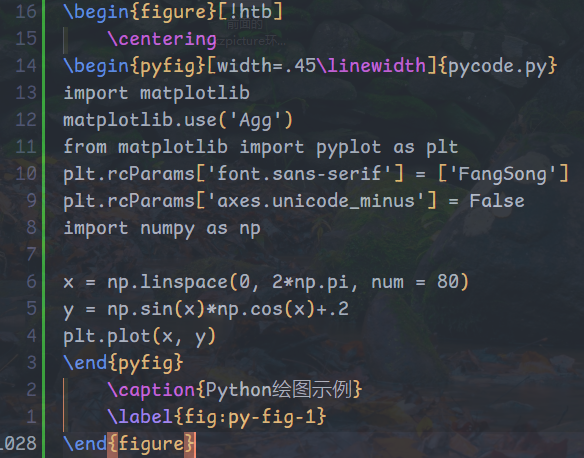
\includegraphics[width=.45\linewidth]{./pics/pyfig_example.png}
\end{center}

如果你实在是需要缩进,那么在这里我推荐另外一种一种可以使用缩进的方法;把\cmd{pyfig}环境连同其内部代码保存在另外一个文件中,
比如这里我保存为\cmd{pycode.mpl},然后在\cmd{figure}环境中使用\cmd{\input{pycode.mpl}}引入此部分的代码。如下:
\begin{codeprint}
\begin{figure}
    \centering
    \input{./data/pycode.mpl}
    \caption{Python Figure}
    \label{fig:pyfig-1}
\end{figure}
\end{codeprint}
\end{leftbar}


\subsection{mathematica}
其实使用mathematica进行绘图这个部分和前面的使用Python绘图是差不多的,zTikZ提供了一个
\index{\cmd{mmafig}}环境用于使用mathematica绘图. 与之前的\cmd{pyfig}环境不同的是,此时你需要手动加入
图片的保存路径;路径的前缀为:\cmd{./ztikz_output/mma_data/<figure name>}. 为何这里这个部分
我不使用zTikZ自动完成? 由于mathematica绘图代码中可能存在着多辐图形的情况,需要使用\cmd{Show}命令
组合成为一个图,那么这个组合方式就是千变万化的了。所以为了给用户提供给更多的自由操作的空间。
这里的图片保存命令由用户自己书写. 并且上述的\cmd{<figure name>}只能写为\cmd{<wls script name>.pdf}
的形式;比如你的WolframScript脚本名称为\cmd{mma_1.wls},那么你的\cmd{<figure name>}只能写为
\cmd{mma_1.wls.pdf},其中的图片格式可以自己指定,比如为\cmd{.png, .jpg, .mbp}等. 此环境同样是加入了Cache机制的,
下面给出一个具体的使用案例:

\begin{codeprint}
\begin{mmafig}[width=.4\linewidth]{mma_1.wls}
    plotFunction[fun_, xlimits_, ylimits_] := ContourPlot[fun, 
        xlimits, ylimits,
        ContourStyle->{
            RGBColor["#00C0A3"], 
            Thickness[0.004]
        },
        AspectRatio->((xlimits[[2]]//Abs) + (xlimits[[3]]//Abs))/((ylimits[[2]]//Abs) + (ylimits[[3]]//Abs)), 
        AxesOrigin->{0,0}, 
        Axes->True,
        Frame->False,
        AxesStyle->Arrowheads[{0, 0.03}],
        AxesLabel->{"x", "y"},
        PlotRange -> Full
    ]
    
    xlimits = {x, -3, 6};
    ylimits = {y, -4, 5};
    fp1 = plotFunction[y==Sin[x], xlimits, ylimits];
    fp2 = plotFunction[x^2/4 + y^2/3 == 5, {x, -5, 5}, {y, -5, 5}];
    
    figure = Show[fp2, fp1];
    (* 1.保存的图片格式为:*.wls.pdf; 2.保存路径在:./ztikz_output/mma_data *)
    Export["./ztikz_output/mma_data/mma_1.wls.pdf", figure];
\end{mmafig}
\end{codeprint}

因为mathematica中的代码是允许用户自由添加缩进的,所以你可以自己添加Mathematica代码的缩进.
和前面的Python绘图代码类似,你可以把此部分代码保存在一个单独的文件中,然后通过\cmd{\input}
进行引入,这里不再给出对应的案例.

\begin{leftbar}
\textbullet 注意空格与Tab,如果源代码中有Tab,那么zTikZ在进行此环境的抄录时会把原本
的Tab转义为 \verb|^^I|,从而造成Mathematica源代码的错误, 比如你可能会看到你的源代码
抄录后变成了下面的样子:
\begin{verbatim}
^^IContourStyle->{
^^I^^IRGBColor["#00C0A3"], 
^^I},
\end{verbatim}

\textbullet 同时注意Mathematica中注释的写法, 不是\verb|(* something*)|, 而是\verb|(* something *)|,
也就是你的注释不能够紧挨着 \verb|*|, 否则会造成mathematica script的解析错误.

\textbullet 由于WolframScript的限制,对应的Mathematica脚本的后缀只能为:\cmd{.wls},否则WolframScript
无法识别此脚本,也就不会去执行此脚本了.
\end{leftbar}


\begin{figure}[!htb]
    \centering
    \begin{mmafig}[width=.5\linewidth]{mma_1.wls}
        plotFunction[fun_, xlimits_, ylimits_] := ContourPlot[fun, 
            xlimits, ylimits,
            ContourStyle->{
                RGBColor["#00C0A3"], 
                Thickness[0.004]
            },
            AspectRatio->((xlimits[[2]]//Abs) + (xlimits[[3]]//Abs))/((ylimits[[2]]//Abs) + (ylimits[[3]]//Abs)), 
            AxesOrigin->{0,0}, 
            Axes->True,
            Frame->False,
            AxesStyle->Arrowheads[{0, 0.03}],
            AxesLabel->{"x", "y"},
            PlotRange -> Full
        ]
        
        xlimits = {x, -3, 6};
        ylimits = {y, -4, 5};
        fp1 = plotFunction[y==Sin[x], xlimits, ylimits];
        fp2 = plotFunction[x^2/4 + y^2/3 == 5, {x, -5, 5}, {y, -5, 5}];
        
        figure = Show[fp2, fp1];
        (* 1.保存的图片格式为:*.wls.pdf; 2.保存路径在:./ztikz_output/mma_data *)
        Export["./ztikz_output/mma_data/mma_1.wls.pdf", figure];
    \end{mmafig}
    \caption{Mathematica 绘图示例}
    \label{fig:mma-fig-1}
\end{figure}

同样的你可以使用Mathematica绘制3维图形\Footnote{由于目前的Mathematica不支持输出3维矢量图,所以想要 
是你的3维图像显得更加的清晰,可以调节图像的分辨率.}。目前zTikZ仅支持插入静态图片,后续可能会考虑加入 
动态图片的支持功能,就行另外一个开源矢量图象绘制软件\href{https://asymptote.sourceforge.io/}{Asymptote}
中的\cmd{.prc}文件一样. 但是要是的PDF支持动态图形,首先你的PDF阅读器必须支持JavaScript,常见的
这种类型的PDF阅读器就是Adobe家的Acrobat了.

\begin{figure}[!htb]
    \centering
    \input{./data/mma_2.wls}
    \caption{Mathematica绘图示例 2}
    \label{fig:mma-fig-2}
\end{figure}


\section{数值计算}
\subsection{xfp}
众说周知,\TeX{}自身的计算能力是比较若的,所以涉及到一定的计算需求时,一般宏包的解决方法都是
使用外部程序,让\TeX{}只负责排版就行了.但是在\LaTeX3项目发展了这么久之后,也做出了一些令人 
惊喜的结果。这里我们主要介绍\LaTeX3的 \href{https://www.ctan.org/pkg/xfp}{xfp} 宏包,用于浮点数运算. 

这里说明部分\index{\cmd{xfp}}也许可以解决的痛点: 
\begin{itemize}
    \item 在TikZ绘图中,常常时需要坐标运算的,尽管TikZ提供了一个\cmd{calc}库,但是
        这个库的使用语法总觉得不是那么的自然。于是这个时候你就可以使用\cmd{xfp}宏包.
    \item 在你自定义一些需要用到数值计算的宏命令时,使用\cmd{xfp}宏包是一个比较好的选择.
\end{itemize}

\cmd{xfp}宏包的详细使用教程请参见官方文档,这里不再赘述.

\begin{leftbar}
\noindent zTikZ或者是z\LaTeX{}并不会自动加载\cmd{xfp}宏包,如果你有这方面的需要,请自己加载.
\end{leftbar}

\subsection{python}
上面介绍了Python的绘图功能,这里再引入zTikZ中的浮点数计算部分(Sympy对应的部分应该不能叫浮点数计算了,毕竟Sympy
进行的是精确的计算。)这里使用的浮点数运算主要是基于Python,以及可能的宏包\cmd{numpy}等. zTikZ在调用
此命令是默认载入Python库\cmd{NumPy, SciPy},并且使用\cmd{numpy}中的函数时不用再加上前缀;比如求解$\sin(2.345)$
时,直接使用\cmd{\pyfp{sin(2.345)}}即可,不用写成\cmd{\pyfp{np.sin(2.345)}}.对于库\cmd{SciPy}中的函数
使用方法同理.

zTikZ提供了命令\index{\cmd{\pyfp}}用于浮点数运算, 这部分的结果并不会被缓存,也就是说每次编译此文档时,Python都会重新
计算此部分的结果. \cmd{\pyfp}的参数说明如下:

\begin{codeprint}
\pyfig{<expression>}
\end{codeprint}

下面给出一个使用样例:
\begin{codeprint}
\pyfp{0.9**10}
\end{codeprint}

\[
    0.9^{10} = \pyfp{0.9**10}
\]


\subsection{mathematica}
使用Mathematica进行数值计算这一部分和后面的\index{\cmd{\wolfram}}指令是有一部分重合的,详细的使用参见后面一节的
``符号计算'', 所以这一部分我们就在后面介绍.


\section{符号计算}
符号计算是区别于数值计算的,上述的数值计算章节应该也有介绍; 但在介绍zTikZ中的符号计算模块之前先给出一个
符号计算的定义,以下定义摘自wiki:

\begin{leftbar}
\kaishu 数学和计算机科学中,计算机代数或符号计算或代数计算,是研究、开发用于操作表达式等数学对象的算法与软件的科学领域。
这通常被视为是运算科学的一个子领域,但运算科学一般基于近似浮点数的数值计算,而符号计算则使用含变量的表达式进行精确计算,
其中变量没有赋值。 执行符号计算的软件系统称为计算机代数系统(computer algebra system, CAS),``系统''暗示了软件的复杂性,
其中至少包括一种在计算机中表示数学数据的方法、一种编程语言(通常异于用于实现的语言)、一种专门的内存管理器、
一套供输入输出表达式的用户界面、一大套用于通常运算的子程序,如表达式简化、能实现链式法则、多项式因式分解、
不定积分等等的求导算法。
\end{leftbar}

当前流行的计算机代数系统主要有:
\begin{multicols}{2}
    \begin{itemize}
    \item mathHandbook.com
    \item Sagemath
    \item Mathematica
    \item Maple
    \item MAGMA
    \item Maxima
    \item GAP
    \item PARI/GP
    \item Meditor
    \item MuPAD
    \item Mathomatic
    \item Xcas/Giac
    \item Yacas
    \item Mate
    \end{itemize}
\end{multicols}

zTikZ主要提供一个和Mathematica(假如你已经购买了该软件),以及Pyhton的Sympy模块的符号计算接口.
后续可能会开发一个统一的接口用于\TeX{}和外部程序的交互.

\subsection{python/sympy}
Python的Sympy是一个\textbf{免费,开源,轻量}的符号计算模块,其官网上有着详细的\href{https://docs.sympy.org/latest/tutorials/intro-tutorial/index.html}{教程}。
所以这里便不再赘述其语法,重点介绍zTikZ中提供的几个接口(命令),用于和Sympy交互.

zTikZ中针对Sympy提供了命令:\index{\cmd{\sympy}},其参数格式为:

\begin{codeprint}
\sympy{<expression>}
\end{codeprint}

和之前的使用Python进行数值计算不同的是,zTikZ针对此命令提供了Cache机制,此命令对应的结果会被保存在文件:
\cmd{./ztikz_output/python_data/sympy_<index>.out}文件中. 此文件名中的\cmd{<index>}表示的是对应的
符号计算表达式的序号. 

\cmd{\sympy}命令的运算结果被保存在文件中之后,通过\cmd{\input}命令把对应的运算结果导入到\TeX{}的输出流(文档)中,
由于默认的情况下此结果包含数学公式中的上下标:\cmd{^, _, ...}等, 所以在把其导入到\LaTeX{}源码中时需要放入数学环境中.

zTikZ模块的\cmd{\sympy}命令在进行符号运算时,默认的符号变量有:\cmd{x, y, z, u, v, t},这些变量你不需声明
便可以直接使用; 下面给出使用\cmd{\sympy}命令进行符号计算的部分示例:

\begin{codeprint}
% 定积分
\sympy{integrate(sin(x)/x, (x, -oo, oo))}
% 不定积分
\sympy{integrate( x**8 + cos(7*x) + 6*t, x )}
% 矩阵特征值
\sympy{Matrix([[1, 2], [2, 2]]).eigenvals()}  
% 极限计算
\sympy{limit(sin(x)/x, x, 0)}
\end{codeprint}

计算定积分的例子:
\[
\int_{-\infty}^{+\infty}{\frac{\sin(x)}{x} \;\mathrm{d}x}
    = \sympy{integrate(sin(x)/x, (x, -oo, oo))}      
\]   

或者是计算不定积分的例子:
\[
    \int x^8 + \cos(7x) + 6t\,\mathrm{d}x  
    = \sympy{integrate( x**8 + cos(7*x) + 6*t, x )}    
\]

或者是一个计算特征值的例子:
\[
\mathrm{eig}(\begin{bmatrix}1 & 2\\2 & 2\end{bmatrix})
    = \sympy{Matrix([[1, 2], [2, 2]]).eigenvals()}    
\]

计算极限的例子:
\[
\lim_{x\to 0}{\frac{\sin x}{x}}
    = \sympy{limit(sin(x)/x, x, 0)}    
\]

\begin{leftbar}
\noindent 目前的\cmd{\sympy}命令只支持单行命令的模式,如果你需要使用多行(条)命令来达到计算目的,
请考虑把它们变为一行命令(一条指令).
\end{leftbar}


\subsection{mathematica}
zTikZ模块提供和Mathematica相关的符号计算,数值运算和知识查询接口; 以下的所有命令均具有缓存机制.
\begin{itemize}
    \item \cmd{\wolfram[<option>]{<expression>}}: 使用Mathematica计算此表达式\cmd{<expression>},默认返回
        \TeX{}格式的代码,可以把\cmd{<option>}设为\cmd{text},让其返回一个文本对象. 可以在这个命令中执行
        任何的wolfram指令,但是需要注意的一点是,所有和wolfram相关的命令是不会自动进入数学模式的,需要手动
        添加数学模式的标记.
    \item \cmd{\wolframsolve[<cmd style>]{<expression>}[<varible>][<domain>]}:其中第一个可选参数默认值为:
        \cmd{part},意味着你的命令需要分拆为3个部分:表达式 -- (求解)变量名 -- 求解范围,对应上面的参数,分别填入。
        如果指定第一个参数为\cmd{full},那么此时只需要给出对应的\cmd{<expresion>},不用在指定后续的参数.(毕竟在
        第二个(强制性-Mandatory)参数中就已经包含了这些信息,参见后面的具体使用样例).
    \item \cmd{\wolframdsolve[<cmd style>]{<equation>}[<independent varible>][<dependent variablei>]}:
        此命令用于求解微分方程,其中的第一个可选参数和上面的\cmd{\wolframsolve}的意义一致,不再赘述.第二个参数表示
        要求解的微分方程,第三个参数表示求解的独立变量(函数),最后一个参数表示此微分方程求解函数的自变量.
\end{itemize}

\subsubsection{wolfram}
首先给出\index{\cmd{\wolfram}}命令的部分使用样例:

\begin{codeprint}
\wolfram{Series[Exp[x], {x, 0, 5}]}
\wolfram{LaplaceTransform[t^4 Sin[t],t,s]}  
\wolfram[text]{WolframAlpha["Shanghai population", "ShortAnswer"]} 
\end{codeprint}

函数 $y=\mathrm{e}^x$的5阶Taylor展开式为:
\[
    \wolfram{Series[Exp[x], {x, 0, 5}]}    
\]

函数 $x=t^4 \sin(t)$的Laplace变换为:
\[
    \C{L}[t^4 \sin(t)] = \wolfram{LaplaceTransform[t^4 Sin[t],t,s]}    
\]

在\cmd{\wolfram}指令中执行Mathematica中的\cmd{WolframAlpha}命令进行查询,比如这里查询
上海的人口数量,结果为:\wolfram[text]{WolframAlpha["Shanghai population", "ShortAnswer"]}

这里补充一个使用\cmd{\wolfram}就行数值运算的例子,因为Mathematica 中有着诸多的和数值运算的函数,
这里仅以内置的函数\cmd{N[<expression>]}为例: 

比如我们求解 $\pi$的截取前30小数的近似值为:
\[
    \pi \approx \wolfram{N[Pi, 30]}    
\]

\begin{leftbar}
\noindent 在使用\cmd{\wolfram}命令进行浮点数运算时,只要表达式中含有小数,那么Mathematica就会默认进行浮点数
运算,而不会计算表达式的精确值.
\end{leftbar}

\subsubsection{wolframsolve}
\index{\cmd{\wolframsolve}}命令可以用于多项式方程根的求解以及方程组的求解,并且可以给定求解的范围.
和前面的\cmd{\wolfram}命令类似,此命令\textbf{只}返回求解结果的\TeX{}代码,所以请把此命令置于公式环境中; 
下面给出几个比较简单的求解示例:

\begin{codeprint}
\wolframsolve{x^4 - x^2 - 5 == 0}{x}
\wolframsolve{a x + y == 7 && b x - y == 1}{x, y}
\wolframsolve{x^2 + 2 y^3 == 3681 && x > 0 && y > 0}[x, y][Integers] 
\wolframsolve[full]{x^2 + y^2 == 5^2 && y > x > 0, {x, y}, Integers}  
\end{codeprint}
    
方程 $x^4 - x^2 - 5 == 0$的所有根为:
\[
    \wolframsolve{x^4 - x^2 - 5 == 0}[x]
\]

方程组 $\left\{\begin{aligned}& a x + y == 7\\ & b x - y == 1\end{aligned}\right.$ 的解为:
\[
    \wolframsolve{a x + y == 7 && b x - y == 1}[x, y]
\]

不定方程 $\left\{\begin{aligned}& x^2 + 2 y^3 == 3681 \\ & x > 0, y>0\end{aligned}\right.$ 的整数解为:
\[
    \wolframsolve{x^2 + 2 y^3 == 3681 && x > 0 && y > 0}[x, y][Integers]    
\]

不定方程 $\left\{\begin{aligned}& x^2 + y^2 == 5^2 \\ & x > y > 0\end{aligned}\right.$ 的整数解为:
\[
    \wolframsolve[full]{x^2 + y^2 == 5^2 && y > x > 0, {x, y}, Integers}    
\]

\begin{leftbar}
\noindent 后续可能会考虑加入解的筛选等功能,其实就是根据不同解之间的分隔符 `,'来对返回的字符串进行一个划分.
根据划分的结果生成一个列表,然后采用一个整数进行索引.
\end{leftbar}

\subsubsection{wolframdsolve}
命令\index{\cmd{\wolframdsolve}}和命令\cmd{\wolframsolve}完全相同, 只是这个命令是用于求解微分方程的.
下面是几个示例:

\begin{codeprint}
\wolframdsolve{{y'[x] + y[x] == a*Sin[x], y[0] == 0}}[y[x]][x]   
\wolframdsolve[full]{{y'[x]==Exp[z[x]]+1, z'[x]==y[x]-x}, {y,z}, x}
\end{codeprint}

微分方程 $y' + y = a\sin(x), y(0)=0$的解为:
\[
    \wolframdsolve{{y'[x] + y[x] == a*Sin[x], y[0] == 0}}[y[x]][x]     
\]

非线性系统微分方程组$y'(x) + y(x) = \mathrm{Exp}(z(x))+1, z'(x) = y(x)-x$的解为:
\[
    \wolframdsolve[full]{{y'[x] == Exp[z[x]] + 1, z'[x] == y[x] - x}, {y[x], z[x]}, x}
\]



\chapter{致谢}
\section{(L\raise2.5pt\hbox{a})\TeX{}}
Wiki上对\TeX{}的定义:
\begin{leftbar}
    TeX (\texttt{/t$\varepsilon$x/}), stylized within the system as \TeX{}, is a typesetting system which was designed 
    and written by computer scientist and Stanford University professor \href{https://en.wikipedia.org/wiki/Donald_Knuth}{Donald Knuth} 
    and first released in 1978. \TeX{} is a popular means of typesetting complex mathematical formulae; 
    it has been noted as one of the most sophisticated digital typographical systems.
\end{leftbar}

但是在我看来\TeX{}不仅仅只是一个排版系统,他是一种精神,一种对于美的追求,一种对于细节的关注.
他并不是\cmd{$Word$}那种商业工具,更不是随性MarkDown.(这里不去谈论\textbf{方正}) 在\TeX{}的基础上
建立了一种格式\LaTeX{}, 这种格式更加的人性化,更加的易用. 使得我们普通人也可以使用部分\TeX{}的排版功能.
为何还有人说\LaTeX{}难学呢 ? 假如他用过\TeX{}之后就会明白\LaTeX{} 的平易近人了.


\section{(L\raise2.5pt\hbox{a})\TeX{}社区}
在此还要感谢所有的 \TeX{} 社区,正是因为他们的无私奉献,本系列才能够顺利的完成. 更特别
感谢 \href{https://www.latex-project.org/latex3/}{\LaTeX3} 团队的所有成员.



\addcontentsline{toc}{chapter}{部分名词索引}
\printindex

\end{document}"' ========

! Package tikz Error: Sorry, the system call 'pdflatex -halt-on-error -interact
ion=batchmode -jobname "tikzdata/release-figure0" "\def\tikzexternalrealjob{release}\i
nput{release}"' did NOT result in a usable output file 'tikzdatamain-figure0' (exp
ected one of .pdf:.jpg:.jpeg:.png:). Please verify that you have enabled system
    calls. For pdflatex, this is 'pdflatex -shell-escape'. Sometimes it is also na
med 'write 18' or something like that. Or maybe the command simply failed? Erro
r messages can be found in 'tikzdata/release-figure0.log'. If you continue now, I'l
l try to typeset the picture.
\end{minted}

% 关于此问题我已经在Github上给作者提了\href{https://github.com/maieul/indextools/issues/17}{Issue},
% 同时也在\TeX-SE上发出了\href{https://tex.stackexchange.com/questions/712716/indextools-confilict-with-tikz-library-external}{提问}.
% 可以关注上述的问题找到解决方法.

目前的解决方法有两个:
\begin{itemize}
    \item 取消加载indextools宏包,改用传统的\cmd{makeidx}宏包.(需自行去修改\cmd{zlatex.cls}中的加载项)
    \item 仍然使用此宏包,但是在第一遍(tikz图片还没有缓存时)取消导言区以及文档末尾的如下命令:
  \begin{minted}{latex}
% 导言区
\makeindex[title=Test Title, columns=3]
% 文末
\addcontentsline{toc}{chapter}{部分名词索引}
\printindex
  \end{minted}
  然后在文档的第二次编译时取消两处命令的注释,以此达到正常编译的目的.
\end{itemize}

\section{Plot Gallery}\label{sec:gallery}
\subsection{tikz}
下面我们给出zTikZ这部分命令的一些综合绘图案例:
\begin{leftbar}
\noindent 如果你修改了绘图代码,但是发现得到的pdf中的图像并没有改变,那么极有可能是因为
你指定的精度过高,超出了\TeX{}的内存使用限制.(而且由于采用了external库用于缓存,有可能你在编译时并不会抛出
这个错误) 其实比较耗费内存的点主要有3个:
\begin{itemize}
    \item 指定的精度过高, 一般情况下在区间长度$<5$时指定精度为100就已经足够了
    \item 使用了多个\cmd{\ContourPlot}函数,在默认的精度 100下,多个此函数也可能导致内存超出
    \item 最后一点耗时的点就是\cmd{\ShowIntersecion}命令,可以先用Geogebra得到交点后再使用
        \cmd{\ShowPoint}命令进行点的绘制.
    \item 更严重的如果出现了编译错误,请考虑去掉\cmd{\ShadePlot}命令,或在\cmd{\usepackage[external=false]{ztikz}}
        的情况下使用此命令.
\end{itemize}
\end{leftbar}


\subsubsection{Example 1}
\begin{figure}[!htb]
    \centering
    % show angle 
\tikzset{
    right angle quadrant/.code={
        \pgfmathsetmacro\quadranta{{1,1,-1,-1}[#1-1]}     % Arrays for selecting quadrant
        \pgfmathsetmacro\quadrantb{{1,-1,-1,1}[#1-1]}},
    right angle quadrant=1, % Make sure it is set, even if not called explicitly
    right angle length/.code={\def\rightanglelength{#1}},   % Length of symbol
    right angle length=2ex, % Make sure it is set...
    right angle symbol/.style n args={3}{
        insert path={
            let \p0 = ($(#1)!(#3)!(#2)$) in     % Intersection
                let \p1 = ($(\p0)!\quadranta*\rightanglelength!(#3)$), % Point on base line
                \p2 = ($(\p0)!\quadrantb*\rightanglelength!(#2)$) in % Point on perpendicular line
                let \p3 = ($(\p1)+(\p2)-(\p0)$) in  % Corner point of symbol
            (\p1) -- (\p3) -- (\p2)
        }
    }
}

% main code
\begin{tikzpicture}[scale=.75, >=Latex]
    \ShowGrid[step=1, color=gray, opacity=.5]{(-8, -8); (8, 8)}
    \ShowXYAxis{8}{8}
    % curve
    \ContourPlot[-8:8; -8:8]{x**2/3-y**2/4-1}
    \ContourPlot[-8:8; -8:8][dashed, red]{(x-3.05)**2 + (y-2.18)**2-4.76}
    % points and lines
    \coordinate (A) at (5.69, 6.26);
    \coordinate (B) at (-5, 0);
    \coordinate (C) at (5, 0);
    \coordinate (D) at (3.05, 2.18);
    \draw (A) -- (B) -- (C) -- cycle;
    % angle and 3-lines
    \draw [blue,right angle symbol={A}{1.94,4.06}{D}]; % F
    \draw [blue,right angle symbol={A}{5.21,1.94}{D}]; % E
    \draw [blue,right angle symbol={B}{3.05,0}{D}];    % G
    \draw (D) -- (1.94, 4.06);
    \draw (D) -- (5.21, 1.94);
    \draw (D) -- (3.05, 0);
    \ShowPoint[type=*, color=red]{(A); (B); (C); (D)}[$A$; $F_1$; $F_2$; $o$][below right]
\end{tikzpicture}
    \caption{Parabolic Example}
    \label{fig:1-parabolic}
\end{figure}
\inputminted{latex}{./gallery/example_1.tex}
\newpage

\subsubsection{Example 2}
\begin{figure}[!htb]
    \centering
    \begin{tikzpicture}[yscale=6, xscale=3]
    \ShowGrid{(-2,0); (2,1)}
    % pdf
    \Plot[-2:2][teal]{1/(sqrt(0.2)*sqrt(2*pi))*exp(-(x-0)**2/(2*0.2**2))}
    \Plot[-2:2][orange]{1/(sqrt(0.5)*sqrt(2*pi))*exp(-(x-0)**2/(2*0.5**2))}
    \Plot[-2:2][green]{1/(sqrt(1)*sqrt(2*pi))*exp(-(x-0)**2/(2*1**2))}
    % cdf
    \Plot[-2:2][teal]{0.5*(1+erf((x-0)/(sqrt(0.2)*sqrt(2))))}
    \Plot[-2:2][orange]{0.5*(1+erf((x-0)/(sqrt(0.5)*sqrt(2))))}
    \Plot[-2:2][green]{0.5*(1+erf((x-0)/(sqrt(1)*sqrt(2))))}
    % annotate
    \ShowPoint[radius=0pt]{(-1, 0); (0, 0); (1, 0)}[$\mu-\sigma$; $\mu=0$; $\mu+\sigma$][below]
    \ShowPoint[radius=0pt]{(1, 0.8); (1, 0.6); (1, 0.4)}[
        \textcolor{red}{\rule[1pt]{8pt}{3pt}}\;$\sigma^2=0.2$;
        \textcolor{orange}{\rule[1pt]{8pt}{3pt}}\;$\sigma^2=0.5$;
        \textcolor{green}{\rule[1pt]{8pt}{3pt}}\;$\sigma^2=1$;
    ][right=2em]
    \ShowPoint[radius=0pt]{(-1, 0.8)}[$\displaystyle y = \frac{1}{\sigma\sqrt{2\pi}}\mathrm{Exp}\{-\frac{(x-\mu)^2}{2\sigma^2}\}$]
    \ShowPoint[radius=0pt]{(-1, 0.6)}[$y=\frac12\left(1+\mathrm{Erf}(\frac{x-\mu}{\sigma\sqrt{2}})\right)$]
\end{tikzpicture}
    \caption{Normal-distribution Example}
    \label{fig:2-norm-distribution}
\end{figure}
\inputminted{latex}{./gallery/example_2.tex}
\newpage


\subsubsection{Example 3}
\begin{figure}[!htb]
    \centering
    \begin{tikzpicture}[>=Latex]
    \xAxis[-1][12]
    \yAxis[-1][7]

    \PlotPrecise{plot}{22}
    \Plot[0.75:11][red, thick, opacity=0][type=ball, color=red]{2.5-1/x}

    \PlotPrecise{plot}{22}
    \Plot[0.5:11.5][red, thick, opacity=0][type=ball, color=green]{3+1/x}

    \PlotPrecise{contour}[long]{40}
    \ContourPlot[0:12][dashed]{y-2.5}
    \ContourPlot[0:12][dashed]{y-3}
\end{tikzpicture}
    \caption{Sup and Inf Example}
    \label{fig:3-sup-inf}
\end{figure}
\inputminted{latex}{./gallery/example_3.tex}
\newpage


\subsubsection{Example 4}
\begin{figure}[!htb]
    \centering
    \ExplSyntaxOn
\clist_new:N \l__color_clist
\clist_set:Nn \l__color_clist {red, orange, yellow, green, blue, purple, brown, black}
\newcommand{\colorItem}[1]{
    \clist_item:Nn \l__color_clist {#1}
}
\ExplSyntaxOff
\begin{tikzpicture}[scale=8, >=Latex, font=\scriptsize]
    % plot and annotate
    \node at (.55, 0.15) [left] {$f(x)=\frac{1}{n}\sin(n+5)x$};
    \foreach \i in {6, 7, 8, 9, 10, 11, 12, 13}{
        \Plot[0:pi/3][\colorItem{\fpeval{\i-5}}]{\fpeval{1/\i}*sin(\fpeval{\i+5}*x)}
        \node[color=\colorItem{\fpeval{\i-5}}] at (1, \fpeval{(\i-6)*0.03}) [right] {$n=\i$};
    }
    % axis draw
    \ShowAxis [
        tickStyle=above,    axisColor=gray,
        tickStart=-0.15,    tickEnd=0.18,
        mainStep=0.05,
        mainTickColor=gray, mainTickLabelPosition=left,
        mainTickLength=.5pt,axisRotate=90,
    ]{(-0.18, 0); (0.18, 0)}
    \ShowAxis [
        tickStyle=below,    axisColor=gray,
        tickStart=0,        tickEnd=1.22,
        mainStep=\fpeval{3.1415926/18},
        mainTickColor=gray, subTickLength=0pt, 
        mainTickLength=.5pt, 
        mainTickLabel={\fpeval{\CurrentFp/(3.1415926/18)*10}$^\circ$}
    ]{(0, 0); (1.25, -0)}
\end{tikzpicture}
    \caption{Loop Plot Example}
    \label{fig:4-loop-to-plot-function}
\end{figure}
\inputminted{latex}{./gallery/example_4.tex}
\newpage

\subsubsection{Example 5}
\begin{figure}[!htb]
    \centering
    \begin{tikzpicture}[>=Latex]
    % draw axis
    \xAxis[0][10]
    \yAxis[-3.25][3.25]
    % plot ucntion and  generate discrete points
    \Plot[0:10]{2*sqrt(x)*cos(log(x))*sin(x)}
    \PlotPrecise{plot}{40}
    \Plot[0:10][opacity=0][type=*, color=red]{2*sqrt(x)*cos(log(x))*sin(x)}
    % bar plot
    \BarPlot[x][fill=orange!35!white, bar width=\fpeval{10/40}cm, opacity=.75, very thin, draw=orange]{\gnudata{2}}
\end{tikzpicture}
    \caption{Darboux Example}
    \label{fig:5-darboux-function}
\end{figure}
\inputminted{latex}{./gallery/example_5.tex}
\newpage


\subsubsection{Example 6}
\begin{figure}[!htb]
    \centering
    \begin{tikzpicture}[>=Latex]
    % grid and axis
    \ShowGrid[step=1, color=gray, opacity=.5]{(0, 0); (10, 10)}
    \xAxis[-1][10]      \yAxis[-1][10]
    % plot and points
    \Plot[0:10][red, jump mark right, very thick, xshift=2pt][type=*, opacity=0]{floor(x)}
    \Plot[0:10][dashed, blue]{x}
    \Plot[1:10][dashed, orange]{x-1}
    \PlotPrecise{plot}{11}
    \Plot[0:10][opacity=0, jump mark right][type=o, color=blue]{x}
    \PlotPrecise{plot}{11}
    \Plot[0:10][opacity=0, jump mark right][type=*, color=red]{x-1}
    \ShowPoint[opacity=0]{(2, 9); (2, 8); (2, 7)}[$y=\lfloor x\rfloor$; $y=x$; $y=x-1$][right]
\end{tikzpicture}
    \caption{Stairs Function Example}
    \label{fig:6-stairs-function}
\end{figure}
\inputminted{latex}{./gallery/example_6.tex}
\newpage


\subsubsection{Example 7}
\begin{figure}[!htb]
    \centering
    \begin{tikzpicture}[font=\small, >=Latex, scale=.65]
    %% ==> ztikz draw grid(coordinates)
    \ShowGrid{(-8, -8); (8, 8)}
    \ShowPoint[opacity=0]{(0, 0)}[$O=(0, 0)$][below right=.5em and 1em]
    \ShowAxis {(0, -8); (0, 8)}
    \ShowAxis {(-8, 0); (8, 0)}

    % draw function
    \Plot[-3:3][orange] {2*x+1}
    \Plot[-1:7.6][cyan] {-.9*x+7}

    %% ==> ztikz Plot functions
    % simple 2d-plot
    \PlotPrecise{plot}{1500}
    \Plot[-7:7.8]{3*sin(1/x)}
    \Plot[-1.5:7.5][green, name path=exp] {x*exp(-x)}
    % param plot
    \ParamPlot[0:2*pi][red, name path=ellipse]{7*sin(t), 4*cos(t)}

    %%% ==> Fill region 
    \begin{scope}
        \clip (2, 0) rectangle (8, 1); 
        \fill[pattern=north east lines] plot file{\gnudata{4}};
    \end{scope}
    \begin{scope}
        \clip (-6, 0) rectangle (-2, -2);
        \fill[pattern=crosshatch, pattern color=orange] plot file{\gnudata{3}} -- (-2, 0) -- (-6, 0);
    \end{scope}

    % default tikz unit
    \ShowPoint[color=red]{(-4cm, 4em); (-4cm, 4cm)}[$A_1$=(-4cm, 4em); $A_2$=(-4cm, 4cm)][left]

    % plot shape and other properties
    \ShowPoint[radius=3pt, color=blue, opacity=.5, type=square*, color=cyan] {(-2.380, -3.761)}
    \ShowPoint[color=orange, opacity=1, radius=2pt] {(1.456, 3.912)}

    % ==> find intersection
    \ShowIntersection{exp; ellipse}{2}
    \ShowPoint {(2.068, 5.137); (4.242, 3.181); (6.843, 0.840); (7.324, 0.408)}
        [$p_1$; $p_2$; $p_3$; $p_4$; $p_5$; $p_6$; $p_7$][above]
\end{tikzpicture}
    \caption{Functions and Points Example}
    \label{fig:7-points-function}
\end{figure}
\inputminted{latex}{./gallery/example_7.tex}
\newpage


\subsubsection{Example 8}
\begin{figure}[!htb]
    \centering
    \begin{tikzpicture}[font=\small, >=Latex, scale=.65]
    %% ==> ztikz draw grid(coordinates)
    \ShowGrid{(-8, -8); (8, 8)}
    \ShowPoint{(0, 0)}[$O=(0, 0)$][below right]
    \ShowAxis {(0, -8); (0, 8)}
    \ShowAxis {(-8, 0); (8, 0)}

    % contour plot
    \PlotPrecise{contour}[long]{10}
    \ContourPlot[-8:8; -8:8][thick, red]{x+6}
    \ContourPlot[-8:8; -8:8][thick, red]{y+6}
    \ContourPlot[-8:8; -8:8][thick, blue]{y-6}
    \ContourPlot[-8:8; -8:8][thick, blue]{x-6}
    \PlotPrecise{contour}[long]{100}
    \ContourPlot[-4:4][green]{x**2/9+y**2/4-1}
    \ContourPlot[-7:7; -7:7][teal]{sin(x**2+y**2)-exp(-x*y)}

    % polar plot
    \begin{scope}[xshift=4cm, yshift=-5cm]
        \PolarPlot[0:10*pi][orange]{0.1*t}
    \end{scope}
    \begin{scope}[xshift=-4cm, yshift=5cm]
        \PolarPlot{2*(1-sin(t))}
        \fill[gray, opacity=.5] plot file {\gnudata{8}};
    \end{scope}

    % node annotate
    \ShowPoint[opacity=0]{(-4, 3); (4, 5); (5, -5); (3, -1)}
        [$\rho=2(1-\sin\theta)$; $\sin(x^2+y^2)-\exp(-xy)=0$; $\rho=0.1\theta$; $\frac{x^2}{9} + \frac{y^2}{4}=1$]
\end{tikzpicture}
    \caption{Polar and Contour Example}
    \label{fig:polar-contour-plot}
\end{figure}
\inputminted{latex}{./gallery/example_8.tex}
\newpage


\subsubsection{Example 9}
\begin{figure}[!htb]
    \centering
    \begin{tikzpicture}[>=Latex, font=\small, scale=1.5]
    % basic
    \clip (-6, -1) rectangle (3, 6);
    \ShowAxis{(-8, 0); (3, 0)}      \ShowAxis{(0, -1.5); (0, 6)}
    % functions
    \Plot[-8:5][red]                {exp(x)}
    \Plot[-8:5][blue]               {exp(1)/4*(x+1)**2}
    \Plot[-8:5][green]              {exp(1)*x + (x-1)**2}
    \Plot[-8:5][purple]             {x**2 + 1}
    \Plot[-8:0.95][gray]            {1/(1-x)}
    \Plot[-8:1.95][orange]          {(2+x)/(2-x)}
    \Plot[-8:5]                     {x+1}
    \Plot[-8:8]                     {exp(1)*x}
    \ContourPlot[0:2;-6:6][dashed]  {x-1}
    % points
    \ShowPoint[color=red, radius=1pt]{(-1, 0); (0, 1); (1, 2.71828)}[$A$; $B$; $C$][above left]
\end{tikzpicture}
    \caption{Exp Functions Example}
    \label{fig:9-exp-functions}
\end{figure}
\inputminted{latex}{./gallery/example_9.tex}
\newpage



\subsubsection{Example 10}
\begin{figure}[!htb]
    \centering
    \begin{tikzpicture}[>=Latex, font=\small, scale=1.25]
    % basic
    \clip (-2, -2) rectangle (10, 4);
    \ShowAxis{(-2, 0); (12, 0)}
    \ShowAxis{(0, -2); (0, 4)}

    % functions
    \Plot[-5:12][red]               {log(x)}
    \Plot[0:12][blue]               {(x-1)/x}
    \Plot[0:12][teal]               {2*(x-1)/(x+1)}
    \Plot[-1:12][purple]            {6*(x-1)/(2*x+5)}
    \Plot[-5:12][gray]              {x/exp(1)}
    \Plot[0.1:12][orange]           {0.5*(x-1/x)}
    \Plot[-5:12]                    {x-1}
    \Plot[-5:12][green]             {x**2-x}
    \ContourPlot[-5:12;-6:6][dashed]{y-1}
    % points
    \ShowPoint[color=red, radius=1pt]
            {(1, 0);(2.71828, 1)}
            [$A$; $B$]
            [above left]
\end{tikzpicture}
    \caption{Log Functions Example}
    \label{fig:10-log-function}
\end{figure}
\inputminted{latex}{./gallery/example_10.tex}
\newpage


\subsubsection{Example 11}
\begin{figure}[!htb]
    \centering
    \begin{tikzpicture}[scale=0.5, >=Latex]
    % axis
    \draw[->](-1,0)--(10,0);
    \draw[->](0,-4)--(0,4);
    % plot function
    \draw[domain=-2:2] plot({(\x)^2}, \x);
    \draw[domain=-2:2] plot(\x+1, \x);
\end{tikzpicture}
    \caption{11 Inverse Function Plot-1}
    \label{fig:11-inverse-function-1}
\end{figure}
\inputminted{latex}{./gallery/example_11_1.tex}

\begin{figure}[!htb]
    \centering
    \begin{tikzpicture}[scale=0.5, >=Latex]
    % axis
    \draw[->](0, -1) -- (0, 7);
    \draw[->](-4, 0)   -- (4, 0);
    % plot function
    \draw[domain=-2:2] plot(\x, {(\x)^2});
    \draw[domain=-2:2] plot(\x, \x+1);
\end{tikzpicture}
    \caption{11 Inverse Function Plot-2}
    \label{fig:11-inverse-function-2}
\end{figure}
\inputminted{latex}{./gallery/example_11_2.tex}
\newpage

\subsubsection{Example 12}
\begin{figure}[!htb]
    \centering
    \begin{tikzpicture}[domain=0:4]
    \draw[very thin,color=gray] (-0.1,-1.1) grid (3.9,3.9);
    \draw[->] (-0.2,0) -- (4.2,0) node[right] {$x$};
    \draw[->] (0,-1.2) -- (0,4.2) node[above] {$f(x)$};
    \draw[color=red] plot[id=x] function{x} node[right] {$f(x) =x$};
    \draw[color=blue] plot[id=sin] function{sin(x)} node[right] {$f(x) = \sin x$};
    \draw[color=orange] plot[id=exp] function{0.05*exp(x)} node[right] {$f(x) = \frac{1}{20} \mathrm e^x$};
\end{tikzpicture}
    \caption{12 TikZ Built-in Plot}
    \label{fig:12-tikz-plot}
\end{figure}
\inputminted{latex}{./gallery/example_12.tex}
\newpage

\subsubsection{Example 13}
\begin{figure}[!htb]
    \centering
    % https://texample.net/tikz/examples/polar-coordinates-template/
\begin{tikzpicture}[scale=.7]
    %Circles 
    \foreach \r in {1, 2,...,7}
        \draw[teal, thick] (0,0) circle (\r);    
    \foreach \r in {0.5, 1.5,...,7}
        \draw[gray, thin] (0,0) circle (\r);
    %1° Rays
    \foreach \a in {0, 1,...,359}
        \draw[gray] (\a:7.7) -- (\a:8);
    %5° Rays
    \foreach \a in {0, 5,...,359}
        \draw[gray] (\a:7.5) -- (\a:8);      
    %15° Rays
    \foreach \a in {0, 15,...,359}
        \draw[thick,gray] (\a:1) -- (\a:8); 
    %30° Rays
    \foreach \a in {0, 30,...,359}
        \draw[thick,gray] (0, 0) -- (\a:8);
    %Radius labels (background filled white)
    \foreach \r in {1, 2,...,7}
        \draw (\r,0) node[inner sep=1pt,below=3pt,rectangle,fill=white] {$\r$};
    %Main rays
    \foreach \a in {0, 90,...,359}
        \draw[very thick] (0, 0) -- (\a:8);
    %Angle labels  
    \foreach \a in {0, 15,...,359}
        \draw (\a: 8.5) node {$\a^\circ$};
    %Central point
    \draw[fill=red] (0,0) circle(0.7mm);
    \PolarPlot[0:2*pi][thick, orange]{t}
\end{tikzpicture}
    \caption{13 Polar Plot And Coordinates}
    \label{fig:13-polar-plot}
\end{figure}
\inputminted{latex}{./gallery/example_13.tex}
\newpage


\subsection{Mathematica}
\subsubsection{Example 1}
\begin{figure}[!htb]
    \centering
    % show angle 
\tikzset{
    right angle quadrant/.code={
        \pgfmathsetmacro\quadranta{{1,1,-1,-1}[#1-1]}     % Arrays for selecting quadrant
        \pgfmathsetmacro\quadrantb{{1,-1,-1,1}[#1-1]}},
    right angle quadrant=1, % Make sure it is set, even if not called explicitly
    right angle length/.code={\def\rightanglelength{#1}},   % Length of symbol
    right angle length=2ex, % Make sure it is set...
    right angle symbol/.style n args={3}{
        insert path={
            let \p0 = ($(#1)!(#3)!(#2)$) in     % Intersection
                let \p1 = ($(\p0)!\quadranta*\rightanglelength!(#3)$), % Point on base line
                \p2 = ($(\p0)!\quadrantb*\rightanglelength!(#2)$) in % Point on perpendicular line
                let \p3 = ($(\p1)+(\p2)-(\p0)$) in  % Corner point of symbol
            (\p1) -- (\p3) -- (\p2)
        }
    }
}

% main code
\begin{tikzpicture}[scale=.75, >=Latex]
    \ShowGrid[step=1, color=gray, opacity=.5]{(-8, -8); (8, 8)}
    \ShowXYAxis{8}{8}
    % curve
    \ContourPlot[-8:8; -8:8]{x**2/3-y**2/4-1}
    \ContourPlot[-8:8; -8:8][dashed, red]{(x-3.05)**2 + (y-2.18)**2-4.76}
    % points and lines
    \coordinate (A) at (5.69, 6.26);
    \coordinate (B) at (-5, 0);
    \coordinate (C) at (5, 0);
    \coordinate (D) at (3.05, 2.18);
    \draw (A) -- (B) -- (C) -- cycle;
    % angle and 3-lines
    \draw [blue,right angle symbol={A}{1.94,4.06}{D}]; % F
    \draw [blue,right angle symbol={A}{5.21,1.94}{D}]; % E
    \draw [blue,right angle symbol={B}{3.05,0}{D}];    % G
    \draw (D) -- (1.94, 4.06);
    \draw (D) -- (5.21, 1.94);
    \draw (D) -- (3.05, 0);
    \ShowPoint[type=*, color=red]{(A); (B); (C); (D)}[$A$; $F_1$; $F_2$; $o$][below right]
\end{tikzpicture}
    \caption{1 Plot Stoke}
    \label{fig:1-plot-stoke}
\end{figure}
\inputminted{mathematica}{./gallery/example_1.wls}
\newpage


\subsubsection{Example 2}
\begin{figure}[!htb]
    \centering
    \begin{tikzpicture}[yscale=6, xscale=3]
    \ShowGrid{(-2,0); (2,1)}
    % pdf
    \Plot[-2:2][teal]{1/(sqrt(0.2)*sqrt(2*pi))*exp(-(x-0)**2/(2*0.2**2))}
    \Plot[-2:2][orange]{1/(sqrt(0.5)*sqrt(2*pi))*exp(-(x-0)**2/(2*0.5**2))}
    \Plot[-2:2][green]{1/(sqrt(1)*sqrt(2*pi))*exp(-(x-0)**2/(2*1**2))}
    % cdf
    \Plot[-2:2][teal]{0.5*(1+erf((x-0)/(sqrt(0.2)*sqrt(2))))}
    \Plot[-2:2][orange]{0.5*(1+erf((x-0)/(sqrt(0.5)*sqrt(2))))}
    \Plot[-2:2][green]{0.5*(1+erf((x-0)/(sqrt(1)*sqrt(2))))}
    % annotate
    \ShowPoint[radius=0pt]{(-1, 0); (0, 0); (1, 0)}[$\mu-\sigma$; $\mu=0$; $\mu+\sigma$][below]
    \ShowPoint[radius=0pt]{(1, 0.8); (1, 0.6); (1, 0.4)}[
        \textcolor{red}{\rule[1pt]{8pt}{3pt}}\;$\sigma^2=0.2$;
        \textcolor{orange}{\rule[1pt]{8pt}{3pt}}\;$\sigma^2=0.5$;
        \textcolor{green}{\rule[1pt]{8pt}{3pt}}\;$\sigma^2=1$;
    ][right=2em]
    \ShowPoint[radius=0pt]{(-1, 0.8)}[$\displaystyle y = \frac{1}{\sigma\sqrt{2\pi}}\mathrm{Exp}\{-\frac{(x-\mu)^2}{2\sigma^2}\}$]
    \ShowPoint[radius=0pt]{(-1, 0.6)}[$y=\frac12\left(1+\mathrm{Erf}(\frac{x-\mu}{\sigma\sqrt{2}})\right)$]
\end{tikzpicture}
    \caption{2 3D Plot}
    \label{fig:2-3d-plot}
\end{figure}
\inputminted{mathematica}{./gallery/example_2.wls}
\newpage


\subsubsection{Example 3}
\begin{figure}[!htb]
    \centering
    \begin{tikzpicture}[>=Latex]
    \xAxis[-1][12]
    \yAxis[-1][7]

    \PlotPrecise{plot}{22}
    \Plot[0.75:11][red, thick, opacity=0][type=ball, color=red]{2.5-1/x}

    \PlotPrecise{plot}{22}
    \Plot[0.5:11.5][red, thick, opacity=0][type=ball, color=green]{3+1/x}

    \PlotPrecise{contour}[long]{40}
    \ContourPlot[0:12][dashed]{y-2.5}
    \ContourPlot[0:12][dashed]{y-3}
\end{tikzpicture}
    \caption{3 Interval Plot}
    \label{fig:3-interval-plot}
\end{figure}
\inputminted{mathematica}{./gallery/example_3.wls}
\newpage


\subsubsection{Example 4}
\begin{figure}[!htb]
    \centering
    \ExplSyntaxOn
\clist_new:N \l__color_clist
\clist_set:Nn \l__color_clist {red, orange, yellow, green, blue, purple, brown, black}
\newcommand{\colorItem}[1]{
    \clist_item:Nn \l__color_clist {#1}
}
\ExplSyntaxOff
\begin{tikzpicture}[scale=8, >=Latex, font=\scriptsize]
    % plot and annotate
    \node at (.55, 0.15) [left] {$f(x)=\frac{1}{n}\sin(n+5)x$};
    \foreach \i in {6, 7, 8, 9, 10, 11, 12, 13}{
        \Plot[0:pi/3][\colorItem{\fpeval{\i-5}}]{\fpeval{1/\i}*sin(\fpeval{\i+5}*x)}
        \node[color=\colorItem{\fpeval{\i-5}}] at (1, \fpeval{(\i-6)*0.03}) [right] {$n=\i$};
    }
    % axis draw
    \ShowAxis [
        tickStyle=above,    axisColor=gray,
        tickStart=-0.15,    tickEnd=0.18,
        mainStep=0.05,
        mainTickColor=gray, mainTickLabelPosition=left,
        mainTickLength=.5pt,axisRotate=90,
    ]{(-0.18, 0); (0.18, 0)}
    \ShowAxis [
        tickStyle=below,    axisColor=gray,
        tickStart=0,        tickEnd=1.22,
        mainStep=\fpeval{3.1415926/18},
        mainTickColor=gray, subTickLength=0pt, 
        mainTickLength=.5pt, 
        mainTickLabel={\fpeval{\CurrentFp/(3.1415926/18)*10}$^\circ$}
    ]{(0, 0); (1.25, -0)}
\end{tikzpicture}
    \caption{4 Stream Plot}
    \label{fig:4-stream-plot}
\end{figure}
\inputminted{mathematica}{./gallery/example_4.wls}
\newpage

\subsubsection{Example 5}
\begin{figure}[!htb]
    \centering
    \begin{tikzpicture}[>=Latex]
    % draw axis
    \xAxis[0][10]
    \yAxis[-3.25][3.25]
    % plot ucntion and  generate discrete points
    \Plot[0:10]{2*sqrt(x)*cos(log(x))*sin(x)}
    \PlotPrecise{plot}{40}
    \Plot[0:10][opacity=0][type=*, color=red]{2*sqrt(x)*cos(log(x))*sin(x)}
    % bar plot
    \BarPlot[x][fill=orange!35!white, bar width=\fpeval{10/40}cm, opacity=.75, very thin, draw=orange]{\gnudata{2}}
\end{tikzpicture}
    \caption{5 Hamiltonian Graph}
    \label{fig:5-hamiltonian-graph}
\end{figure}
\inputminted{mathematica}{./gallery/example_5.wls}
\newpage


\subsubsection{Example 6}
\begin{figure}[!htb]
    \centering
    \begin{tikzpicture}[>=Latex]
    % grid and axis
    \ShowGrid[step=1, color=gray, opacity=.5]{(0, 0); (10, 10)}
    \xAxis[-1][10]      \yAxis[-1][10]
    % plot and points
    \Plot[0:10][red, jump mark right, very thick, xshift=2pt][type=*, opacity=0]{floor(x)}
    \Plot[0:10][dashed, blue]{x}
    \Plot[1:10][dashed, orange]{x-1}
    \PlotPrecise{plot}{11}
    \Plot[0:10][opacity=0, jump mark right][type=o, color=blue]{x}
    \PlotPrecise{plot}{11}
    \Plot[0:10][opacity=0, jump mark right][type=*, color=red]{x-1}
    \ShowPoint[opacity=0]{(2, 9); (2, 8); (2, 7)}[$y=\lfloor x\rfloor$; $y=x$; $y=x-1$][right]
\end{tikzpicture}
    \caption{6 statistic Plot}
    \label{fig:6-statistic-plot}
\end{figure}
\inputminted{mathematica}{./gallery/example_6.wls}
\newpage



\subsubsection{Example 7}
\begin{figure}[!htb]
    \centering
    \begin{tikzpicture}[font=\small, >=Latex, scale=.65]
    %% ==> ztikz draw grid(coordinates)
    \ShowGrid{(-8, -8); (8, 8)}
    \ShowPoint[opacity=0]{(0, 0)}[$O=(0, 0)$][below right=.5em and 1em]
    \ShowAxis {(0, -8); (0, 8)}
    \ShowAxis {(-8, 0); (8, 0)}

    % draw function
    \Plot[-3:3][orange] {2*x+1}
    \Plot[-1:7.6][cyan] {-.9*x+7}

    %% ==> ztikz Plot functions
    % simple 2d-plot
    \PlotPrecise{plot}{1500}
    \Plot[-7:7.8]{3*sin(1/x)}
    \Plot[-1.5:7.5][green, name path=exp] {x*exp(-x)}
    % param plot
    \ParamPlot[0:2*pi][red, name path=ellipse]{7*sin(t), 4*cos(t)}

    %%% ==> Fill region 
    \begin{scope}
        \clip (2, 0) rectangle (8, 1); 
        \fill[pattern=north east lines] plot file{\gnudata{4}};
    \end{scope}
    \begin{scope}
        \clip (-6, 0) rectangle (-2, -2);
        \fill[pattern=crosshatch, pattern color=orange] plot file{\gnudata{3}} -- (-2, 0) -- (-6, 0);
    \end{scope}

    % default tikz unit
    \ShowPoint[color=red]{(-4cm, 4em); (-4cm, 4cm)}[$A_1$=(-4cm, 4em); $A_2$=(-4cm, 4cm)][left]

    % plot shape and other properties
    \ShowPoint[radius=3pt, color=blue, opacity=.5, type=square*, color=cyan] {(-2.380, -3.761)}
    \ShowPoint[color=orange, opacity=1, radius=2pt] {(1.456, 3.912)}

    % ==> find intersection
    \ShowIntersection{exp; ellipse}{2}
    \ShowPoint {(2.068, 5.137); (4.242, 3.181); (6.843, 0.840); (7.324, 0.408)}
        [$p_1$; $p_2$; $p_3$; $p_4$; $p_5$; $p_6$; $p_7$][above]
\end{tikzpicture}
    \caption{7 Stream Plot}
    \label{fig:7-stream-plot}
\end{figure}
\inputminted{mathematica}{./gallery/example_7.wls}
\newpage

\subsubsection{Example 8}
\begin{figure}[!htb]
    \centering
    \begin{tikzpicture}[font=\small, >=Latex, scale=.65]
    %% ==> ztikz draw grid(coordinates)
    \ShowGrid{(-8, -8); (8, 8)}
    \ShowPoint{(0, 0)}[$O=(0, 0)$][below right]
    \ShowAxis {(0, -8); (0, 8)}
    \ShowAxis {(-8, 0); (8, 0)}

    % contour plot
    \PlotPrecise{contour}[long]{10}
    \ContourPlot[-8:8; -8:8][thick, red]{x+6}
    \ContourPlot[-8:8; -8:8][thick, red]{y+6}
    \ContourPlot[-8:8; -8:8][thick, blue]{y-6}
    \ContourPlot[-8:8; -8:8][thick, blue]{x-6}
    \PlotPrecise{contour}[long]{100}
    \ContourPlot[-4:4][green]{x**2/9+y**2/4-1}
    \ContourPlot[-7:7; -7:7][teal]{sin(x**2+y**2)-exp(-x*y)}

    % polar plot
    \begin{scope}[xshift=4cm, yshift=-5cm]
        \PolarPlot[0:10*pi][orange]{0.1*t}
    \end{scope}
    \begin{scope}[xshift=-4cm, yshift=5cm]
        \PolarPlot{2*(1-sin(t))}
        \fill[gray, opacity=.5] plot file {\gnudata{8}};
    \end{scope}

    % node annotate
    \ShowPoint[opacity=0]{(-4, 3); (4, 5); (5, -5); (3, -1)}
        [$\rho=2(1-\sin\theta)$; $\sin(x^2+y^2)-\exp(-xy)=0$; $\rho=0.1\theta$; $\frac{x^2}{9} + \frac{y^2}{4}=1$]
\end{tikzpicture}
    \caption{8 3D Sphere}
    \label{fig:8-3d-sphere}
\end{figure}
\inputminted{mathematica}{./gallery/example_8.wls}
\newpage


\subsection{Python}
\subsubsection{Example 1}
\begin{figure}[!htb]
    \centering
    % show angle 
\tikzset{
    right angle quadrant/.code={
        \pgfmathsetmacro\quadranta{{1,1,-1,-1}[#1-1]}     % Arrays for selecting quadrant
        \pgfmathsetmacro\quadrantb{{1,-1,-1,1}[#1-1]}},
    right angle quadrant=1, % Make sure it is set, even if not called explicitly
    right angle length/.code={\def\rightanglelength{#1}},   % Length of symbol
    right angle length=2ex, % Make sure it is set...
    right angle symbol/.style n args={3}{
        insert path={
            let \p0 = ($(#1)!(#3)!(#2)$) in     % Intersection
                let \p1 = ($(\p0)!\quadranta*\rightanglelength!(#3)$), % Point on base line
                \p2 = ($(\p0)!\quadrantb*\rightanglelength!(#2)$) in % Point on perpendicular line
                let \p3 = ($(\p1)+(\p2)-(\p0)$) in  % Corner point of symbol
            (\p1) -- (\p3) -- (\p2)
        }
    }
}

% main code
\begin{tikzpicture}[scale=.75, >=Latex]
    \ShowGrid[step=1, color=gray, opacity=.5]{(-8, -8); (8, 8)}
    \ShowXYAxis{8}{8}
    % curve
    \ContourPlot[-8:8; -8:8]{x**2/3-y**2/4-1}
    \ContourPlot[-8:8; -8:8][dashed, red]{(x-3.05)**2 + (y-2.18)**2-4.76}
    % points and lines
    \coordinate (A) at (5.69, 6.26);
    \coordinate (B) at (-5, 0);
    \coordinate (C) at (5, 0);
    \coordinate (D) at (3.05, 2.18);
    \draw (A) -- (B) -- (C) -- cycle;
    % angle and 3-lines
    \draw [blue,right angle symbol={A}{1.94,4.06}{D}]; % F
    \draw [blue,right angle symbol={A}{5.21,1.94}{D}]; % E
    \draw [blue,right angle symbol={B}{3.05,0}{D}];    % G
    \draw (D) -- (1.94, 4.06);
    \draw (D) -- (5.21, 1.94);
    \draw (D) -- (3.05, 0);
    \ShowPoint[type=*, color=red]{(A); (B); (C); (D)}[$A$; $F_1$; $F_2$; $o$][below right]
\end{tikzpicture}
    \caption{1 Step Demo}
    \label{fig:1-step-demo}
\end{figure}
\inputminted{python}{./gallery/example_1.mpl}
\newpage


\subsubsection{Example 2}
\begin{figure}[!htb]
    \centering
    \begin{tikzpicture}[yscale=6, xscale=3]
    \ShowGrid{(-2,0); (2,1)}
    % pdf
    \Plot[-2:2][teal]{1/(sqrt(0.2)*sqrt(2*pi))*exp(-(x-0)**2/(2*0.2**2))}
    \Plot[-2:2][orange]{1/(sqrt(0.5)*sqrt(2*pi))*exp(-(x-0)**2/(2*0.5**2))}
    \Plot[-2:2][green]{1/(sqrt(1)*sqrt(2*pi))*exp(-(x-0)**2/(2*1**2))}
    % cdf
    \Plot[-2:2][teal]{0.5*(1+erf((x-0)/(sqrt(0.2)*sqrt(2))))}
    \Plot[-2:2][orange]{0.5*(1+erf((x-0)/(sqrt(0.5)*sqrt(2))))}
    \Plot[-2:2][green]{0.5*(1+erf((x-0)/(sqrt(1)*sqrt(2))))}
    % annotate
    \ShowPoint[radius=0pt]{(-1, 0); (0, 0); (1, 0)}[$\mu-\sigma$; $\mu=0$; $\mu+\sigma$][below]
    \ShowPoint[radius=0pt]{(1, 0.8); (1, 0.6); (1, 0.4)}[
        \textcolor{red}{\rule[1pt]{8pt}{3pt}}\;$\sigma^2=0.2$;
        \textcolor{orange}{\rule[1pt]{8pt}{3pt}}\;$\sigma^2=0.5$;
        \textcolor{green}{\rule[1pt]{8pt}{3pt}}\;$\sigma^2=1$;
    ][right=2em]
    \ShowPoint[radius=0pt]{(-1, 0.8)}[$\displaystyle y = \frac{1}{\sigma\sqrt{2\pi}}\mathrm{Exp}\{-\frac{(x-\mu)^2}{2\sigma^2}\}$]
    \ShowPoint[radius=0pt]{(-1, 0.6)}[$y=\frac12\left(1+\mathrm{Erf}(\frac{x-\mu}{\sigma\sqrt{2}})\right)$]
\end{tikzpicture}
    \caption{2 Histogram Demo}
    \label{fig:2-histogram-demo}
\end{figure}
\inputminted{python}{./gallery/example_2.mpl}
\newpage


\subsubsection{Example 3}
\begin{figure}[!htb]
    \centering
    \begin{tikzpicture}[>=Latex]
    \xAxis[-1][12]
    \yAxis[-1][7]

    \PlotPrecise{plot}{22}
    \Plot[0.75:11][red, thick, opacity=0][type=ball, color=red]{2.5-1/x}

    \PlotPrecise{plot}{22}
    \Plot[0.5:11.5][red, thick, opacity=0][type=ball, color=green]{3+1/x}

    \PlotPrecise{contour}[long]{40}
    \ContourPlot[0:12][dashed]{y-2.5}
    \ContourPlot[0:12][dashed]{y-3}
\end{tikzpicture}
    \caption{3 3D Stem Demo}
    \label{fig:3-3d-stem-demo}
\end{figure}
\inputminted{python}{./gallery/example_3.mpl}
\newpage

\subsubsection{Example 4}
\begin{figure}[!htb]
    \centering
    \ExplSyntaxOn
\clist_new:N \l__color_clist
\clist_set:Nn \l__color_clist {red, orange, yellow, green, blue, purple, brown, black}
\newcommand{\colorItem}[1]{
    \clist_item:Nn \l__color_clist {#1}
}
\ExplSyntaxOff
\begin{tikzpicture}[scale=8, >=Latex, font=\scriptsize]
    % plot and annotate
    \node at (.55, 0.15) [left] {$f(x)=\frac{1}{n}\sin(n+5)x$};
    \foreach \i in {6, 7, 8, 9, 10, 11, 12, 13}{
        \Plot[0:pi/3][\colorItem{\fpeval{\i-5}}]{\fpeval{1/\i}*sin(\fpeval{\i+5}*x)}
        \node[color=\colorItem{\fpeval{\i-5}}] at (1, \fpeval{(\i-6)*0.03}) [right] {$n=\i$};
    }
    % axis draw
    \ShowAxis [
        tickStyle=above,    axisColor=gray,
        tickStart=-0.15,    tickEnd=0.18,
        mainStep=0.05,
        mainTickColor=gray, mainTickLabelPosition=left,
        mainTickLength=.5pt,axisRotate=90,
    ]{(-0.18, 0); (0.18, 0)}
    \ShowAxis [
        tickStyle=below,    axisColor=gray,
        tickStart=0,        tickEnd=1.22,
        mainStep=\fpeval{3.1415926/18},
        mainTickColor=gray, subTickLength=0pt, 
        mainTickLength=.5pt, 
        mainTickLabel={\fpeval{\CurrentFp/(3.1415926/18)*10}$^\circ$}
    ]{(0, 0); (1.25, -0)}
\end{tikzpicture}
    \caption{4 3D Numpy Logo}
    \label{fig:4-numpy-logo}
\end{figure}
\inputminted{python}{./gallery/example_4.mpl}
\newpage



\part{索引与参考}
\printindex


% Appendix
\chapter{TikZ Built-in Functions}
\label{chap:tikz_function_plot}
本节主要截取了TikZ官方文档中的部分内容,主要涵盖TikZ内置函数的绘制的内容。
相信这一部分的内容可以帮助读者更好的理解zTikZ宏包的工作原理,同时也能够使得
zTikZ宏包的使用更加的便捷.

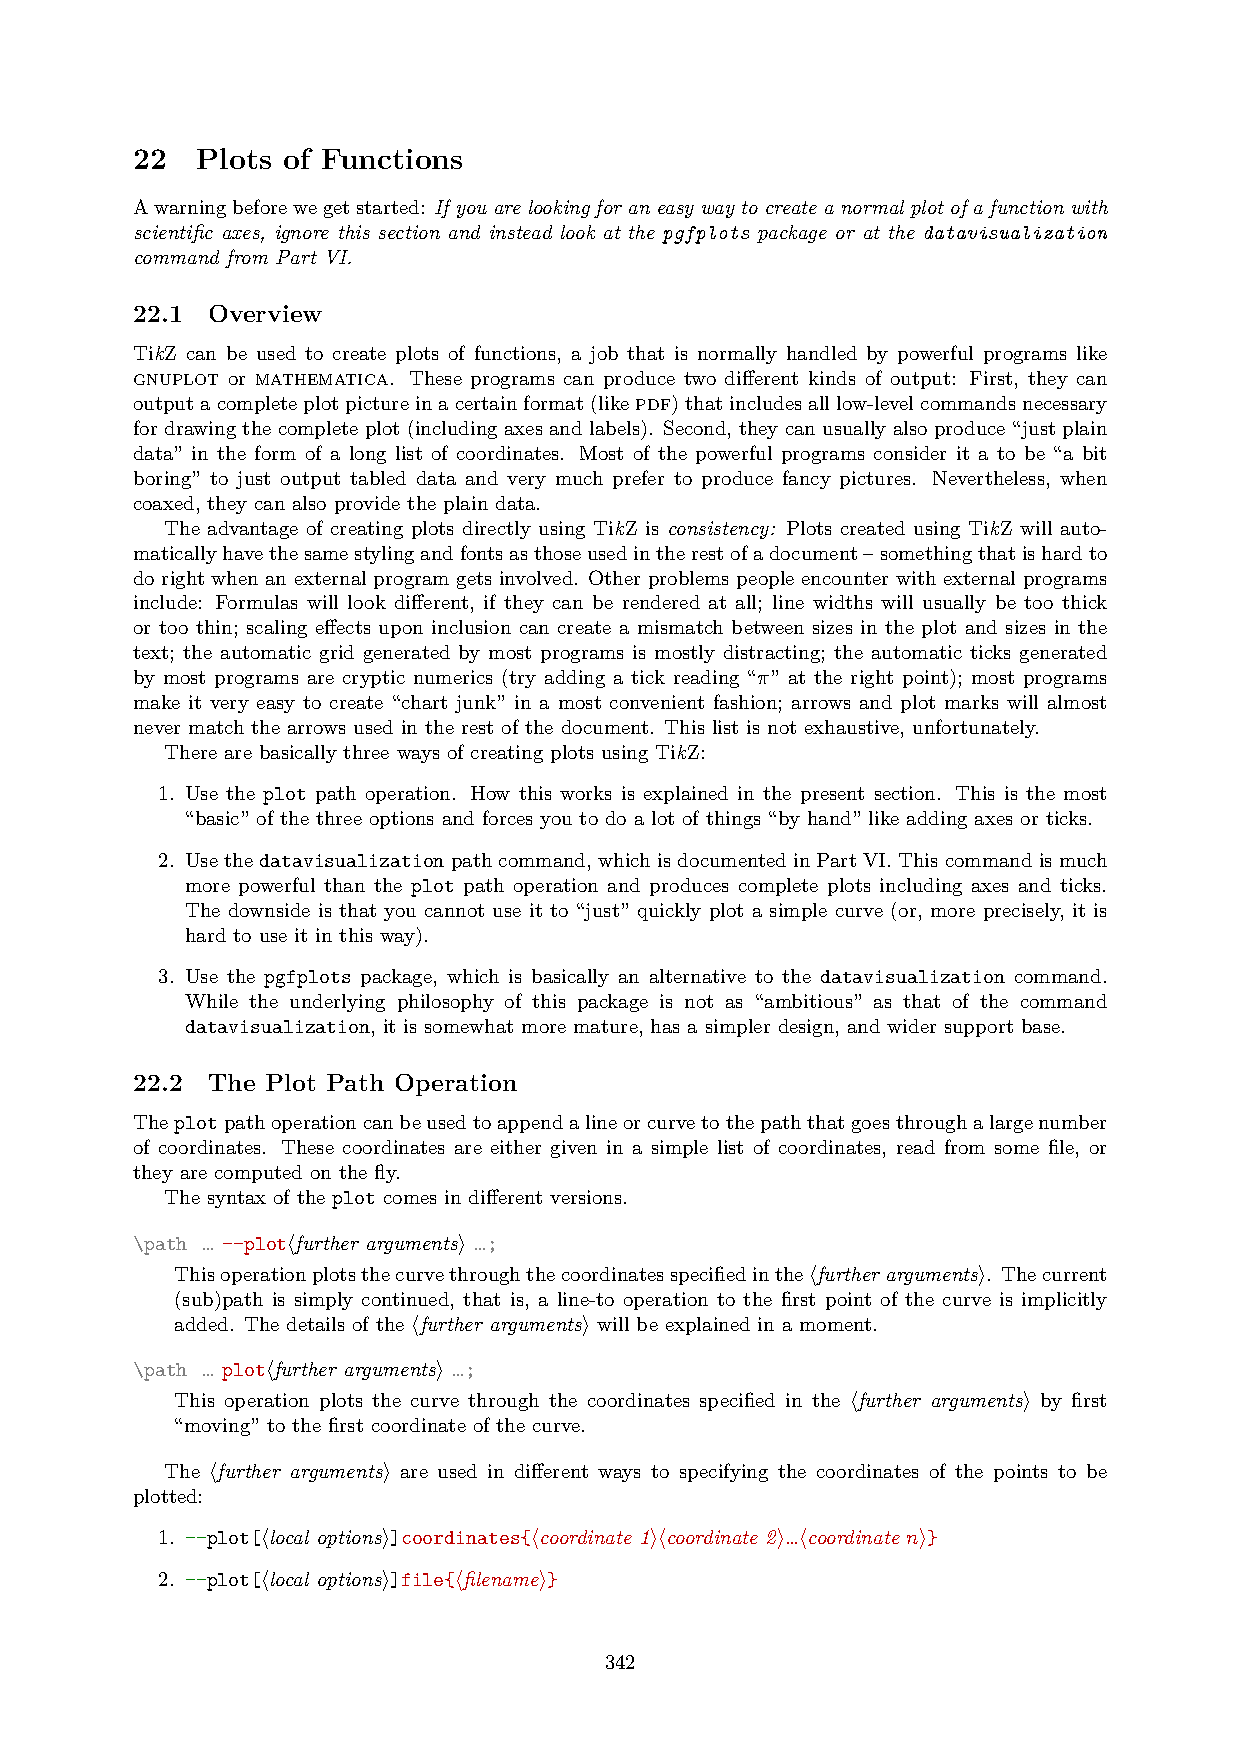
\includepdf[pages=1-11]{tikz_manual.pdf}
\chapter{z\LaTeX{} Implement}
\section{文档选项}
\subsection{Key-Value}
\begin{minted}[linenos=true]{latex}
\cs_new_protected:Npn \zlatex_define_option:n
    { \keys_define:nn { zlatex / option } }
\cs_new_protected:Npn \zlatex_define:nn #1
    { \keys_define:nn { zlatex / #1} }
\cs_new_protected:Npn \zlatex_set:nn #1
    { \keys_set:nn { zlatex / #1 } }
\cs_new_protected:Npn \zlatex_load_after:n #1
    { \AtBeginDocument {#1} }
\end{minted}

\subsection{Load Options}
\begin{minted}[linenos=true]{latex}
\RequirePackage {l3keys2e}
% key-value alias
\cs_new_protected:Npn \zlatex_define_option:n
    { \keys_define:nn { zlatex / option } }
\cs_new_protected:Npn \zlatex_define:nn #1
    { \keys_define:nn { zlatex / #1} }
\cs_new_protected:Npn \zlatex_set:nn #1
    { \keys_set:nn { zlatex / #1 } }
\cs_new_protected:Npn \zlatex_load_after:n #1
    { \AtBeginDocument {#1} }

% setup options for class
\zlatex_define_option:n {
  % zlatex language
  lang            .str_gset:N   =  \g__zlatex_lang_str,
  lang            .initial:n    =  { en },
  hyper           .bool_gset:N  =  \g__zlatex_hyperref_bool,
  hyper           .initial:n    =  { false },
  % class and options
  class           .str_gset:N   = \g__zlatex_subclass_type_str,
  class           .initial:n    = { article },
  classOption     .clist_gset:N = \g__zlatex_subclass_option_clist,
  classOption     .initial:n    = { oneside, 10pt },
  % zlatex options meta key 
  layout          .meta:nn      = {zlatex / layout}{#1},
  mathSpec        .meta:nn      = {zlatex / mathSpec}{#1},
  font            .meta:nn      = {zlatex / font}{#1},
  bib             .meta:nn      = {zlatex / bib}{#1},
  % toc setup
  toc             .multichoice:,
  toc / 2column   .code:n       =  { \zlatex_load_after:n { \RequirePackage[toc]{multitoc} } },
  toc / redef     .code:n       =  { 
      \str_case:VnF \g__zlatex_lang_str {
          {en}{ \zlatex_load_after:n {\renewcommand{\contentsname}{\hfill\bfseries\huge Contents \hfill}} }
          {cn}{ \zlatex_load_after:n {\renewcommand{\contentsname}{\hfill\bfseries\huge 目录     \hfill}} }
      }{\msg_error:nn {zlatex}{option-language}}
  },
  toc / unknown.code:n          =  {
      \msg_new:nnn {zlatex}{option-toc}{Current~toc~option~is~:~'#1'~,default~toc~settings~substitute.}
      \msg_warning:nn {zlatex}{option-toc}
  },
}

% sub-key for each option
\zlatex_define:nn {layout}{
  margin              .bool_gset:N  = \g__zlatex_margin_bool,
  margin              .initial:n    = { false },
  slide               .bool_gset:N  = \g__zlatex_slide_bool,
  slide               .initial:n    = { false },
  aspect              .tl_gset:N    = \g__zlatex_aspectratio_tl,
  aspect              .initial:n    = { 12|9 },
}
\zlatex_define:nn {mathSpec}{
    alias               .bool_gset:N  = \g__zlatex_math_alias_bool,
    alias               .initial:n    = { false },
    envStyle            .tl_gset:N    = \g__zlatex_math_env_style_tl,
    envStyle            .initial:n    = { plain },
    font                .choice:,
    font / newtx        .code:n       = { \zlatex_load_after:n { \RequirePackage{newtxmath} } },
    font / mtpro2       .code:n       = { \zlatex_load_after:n { \RequirePackage[lite, subscriptcorrection, slantedGreek, nofontinfo]{mtpro2} } },
    font / euler        .code:n       = { \zlatex_load_after:n { \RequirePackage[OT1, euler-digits]{eulervm} } },
    font / mathpazo     .code:n       = { \let\rmbefore\rmdefault\zlatex_load_after:n { \RequirePackage{mathpazo} } \let\rmdefault\rmbefore},
    font / unknown      .code:n       = {
        \msg_new:nnn {zlatex}{option-mathfont}{Current~math~font~option~is~:~'#1'~,default~math-font~substitute.}
        \msg_warning:nn {zlatex}{option-mathfont}
    },
}
\zlatex_define:nn {font}{

}
\zlatex_define:nn {bib}{
    source              .str_gset:N   =  \g__zlatex_bib_source_str,
    source              .initial:n    =  { ref.bib },
    backend             .str_gset:N   =  \g__zlatex_bib_backend_str,
    backend             .initial:n    =  { biber },
}

% option setup
\ProcessKeysOptions {zlatex / option}
\NewDocumentCommand{\zlatexSetup}{m}{
    \zlatex_set:nn {option}{#1}
}
\end{minted}

\section{class load}
\begin{minted}[linenos=true]{latex}
% pass clist options main subclass: 'article', 'book', 'ctexbook'
\str_case:VnF \g__zlatex_subclass_type_str {
    {article}{
        \PassOptionsToClass{\g__zlatex_subclass_option_clist}{ article }
        \LoadClass{article}
    }
    {book}{
        \PassOptionsToClass{\g__zlatex_subclass_option_clist}{ book }
        \LoadClass{book}   
    }
    {ctexbook}{
        \str_set:Nn \g__zlatex_lang_str {cn}
        \PassOptionsToClass{\g__zlatex_subclass_option_clist}{ ctexbook }
        \PassOptionsToPackage{quiet}{fontspec}
        \LoadClass{ctexbook}    
    }
}{\relax}
\end{minted}

\section{compile engine}
\begin{minted}[linenos=true]{latex}
% baisc document class and packages option
\msg_new:nnn {zlatex}{compile-engine-pdftex}{Current~compile~engine~is~XETEX,~use~PDFTEX~instead.}
\msg_new:nnn {zlatex}{compile-engine-xetex }{Current~compile~engine~is~PDFTEX,~use~XETEX~instead.}
\str_case:VnF \g__zlatex_lang_str {
    {en} { 
        \sys_if_engine_xetex:TF 
            {\msg_warning:nn {zlatex}{compile-engine-pdftex}}
            {\RequirePackage[utf8]{inputenc}}
        \RequirePackage[T1]{fontenc}
        \RequirePackage[english]{babel}
    }
    {cn} {
        \sys_if_engine_xetex:TF {}{\msg_error:nn {zlatex}{compile-engine-xetex}}
        \PassOptionsToPackage{quiet}{fontspec}
        \PassOptionsToPackage{no-math}{fontspec}
        \str_if_eq:VnF \g__zlatex_subclass_type_str {ctexbook}{
            \RequirePackage[UTF8, heading]{ctex}
            \linespread{1.3}
        }
    }
}{\msg_error:nn {zlatex}{option-language}}   
\end{minted}

\section{Layout}
\subsection{geometry}
\begin{minted}[linenos=true]{latex}
\RequirePackage{geometry}
% page layout 
\if@twoside 
    \geometry{a4paper, left=3cm, right=5.5cm, bottom=3.5cm, footskip=1.5cm, marginparsep=1em}
    \bool_if:NTF \g__zlatex_margin_bool {}{
        \msg_new:nnn {zlatex}{option-page-margin}{No~margin~option~is~only~accessible~in~oneside~layout,~margin~option~is~now~enabled~by~default.} 
        \msg_warning:nn {zlatex}{option-page-margin}
    }
\else 
    \bool_if:NTF \g__zlatex_margin_bool {
        \geometry{a4paper, left=3cm, right=5.5cm, bottom=3.5cm, footskip=1.5cm, marginparsep=1em}
        \dim_gset:Nn \marginparwidth{9.25em}
    }{
        \geometry{a4paper, left=3cm, right=3cm, bottom=3.5cm, footskip=1.5cm, marginparsep=1em}
        \renewcommand{\marginpar}[1]{\leftbar\noindent#1\endleftbar}
    }
\fi
\end{minted}

\subsection{Slide mode}
\begin{minted}{latex}
% slide mode (only in 'oneside' mode)
\exp_args:NNnx \seq_set_split:Nnn \l_tmpa_seq {|}{\g__zlatex_aspectratio_tl}
\bool_if:NTF \g__zlatex_slide_bool {
  \RequirePackage{lastpage}
  \definecolor{slideRed}{HTML}{a30000}
  \definecolor{slideGray}{HTML}{e0e0e0}
  \definecolor{slideWhite}{HTML}{f0f0f0}
  % hook shipout
  \RequirePackage{eso-pic}
  \AddToShipoutPictureBG {
    \AtPageUpperLeft {
      \textcolor{slideRed}{\rule[-1.25em]{.5\paperwidth}{1.25em}}
      \textcolor{slideGray}{\rule[-1.25em]{.5\paperwidth}{1.25em}}
    }
    \AtPageLowerLeft {
      \textcolor{slideRed}{\rule{.35\paperwidth}{1.25em}}
      \textcolor{slideWhite}{\rule{.3\paperwidth}{1.25em}}
      \textcolor{slideGray}{\rule{.35\paperwidth}{1.25em}}
    }
  }
  % layout and mark
  \RequirePackage{titling}
  \IfClassLoadedTF{book}{
    \renewcommand\chaptermark[1]{\markboth{#1}{}}
  }{\relax}
  \renewcommand\sectionmark[1]{\markboth{#1}{}}
  \geometry {
    papersize={\seq_item:Nn \l_tmpa_seq {1}cm, \seq_item:Nn \l_tmpa_seq {2}cm},
    hmargin=1cm,
    vmargin=.65cm,
    head=0.52cm,
    foot=12pt,
    headsep=5pt,
    footskip=15pt
  }
  % init slide mode
  \zlatex_load_after:n {\pagestyle{fancy}}
}{\relax}
\end{minted}

\subsection{fancyhdr}
\begin{minted}[linenos=true]{latex}
% fancy page settings
% fancy page settings
\cs_if_exist_use:NF \theauthor{
  \newcommand{\theauthor}{}
  \newcommand{\thetitle}{}
  \newcommand{\thedate}{}
}

\fancypagestyle{fancy}{
  \fancyhf{}  
  \dim_gset:Nn \headheight{15pt}
  \renewcommand{\headrule}{\hrule width\textwidth}
  % slide mode
  \bool_if:NTF \g__zlatex_slide_bool {
    \def\headrule{}
    \fancyhead[L]{\hbox to .42\paperwidth{\hss\sffamily\textcolor{white}{Section \ \thesection}\;}}
    \fancyhead[R]{\hbox to .42\paperwidth{\;\sffamily\textcolor{slideRed}{\leftmark}\hss}}
    \fancyfoot[L]{\sffamily\textcolor{white}{\theauthor}}
    \fancyfoot[C]{\sffamily\textcolor{slideRed}{\thetitle}}
    \fancyfoot[R]{\sffamily\textcolor{slideRed}{\hbox to .25\paperwidth{\hfill\thedate\kern2.5em\thepage/\pageref{LastPage}}}}
  }{
  % doc mode
    \if@twoside
      \fancyhead[EL]{\leftmark}
      \fancyhead[ER]{\thepage}
      \fancyhead[OL]{\thepage}
      \fancyhead[OR]{\rightmark}
    \else
      \IfClassLoadedTF{book}{
        \fancyhead[L]{\thepage}
        \fancyhead[R]{\rightmark}
      }{
        \fancyhead[L]{\thepage}
        \fancyhead[R]{\leftmark}
      }
    \fi
  }
}

% front and main matter cmds in book class
\IfClassLoadedTF{book}{
    \renewcommand\frontmatter{
        \cleardoublepage
        \pagestyle{plain}
        \@mainmatterfalse
        \pagenumbering{Roman}
    }
    \renewcommand\mainmatter{
        \cleardoublepage
        \pagestyle{fancy}
        \@mainmattertrue
        \pagenumbering{arabic}
    }
}{\relax}
\end{minted}


\section{math}
\subsection{math env theme}
\begin{minted}[linenos=true]{latex}
% color spec for zlatex
\zlatex_define:nn {color}{
    % structure color
    link            .tl_set:N     =  \l__zlatex_link_color_tl,
    link            .initial:n    =  { purple },
    cite            .tl_set:N     =  \l__zlatex_cite_color_tl,
    cite            .initial:n    =  { teal },
    url             .tl_set:N     =  \l__zlatex_url_color_tl,
    url             .initial:n    =  { RoyalRed  },
    chapter         .tl_set:N     =  \l__zlatex_chapter_color_tl,
    chapter         .initial:n    =  { RoyalRed },  
    chapter-rule    .tl_set:N     =  \l__zlatex_chapter_rule_color_tl,
    chapter-rule    .initial:n    =  { black },
    % math envs      color
    axiom           .tl_set:N     =  \l__zlatex_axiom_color_tl,
    axiom           .initial:n    =  { mathaxiomColor },
    definition      .tl_set:N     =  \l__zlatex_definition_color_tl,
    definition      .initial:n    =  { mathdefinitionColor },
    theorem         .tl_set:N     =  \l__zlatex_theorem_color_tl,
    theorem         .initial:n    =  { maththeoremColor },
    lemma           .tl_set:N     =  \l__zlatex_lemma_color_tl,
    lemma           .initial:n    =  { mathlemmaColor },
    corollary       .tl_set:N     =  \l__zlatex_corollary_color_tl,
    corollary       .initial:n    =  { mathcorollaryColor },
    proposition     .tl_set:N     =  \l__zlatex_proposition_color_tl,
    proposition     .initial:n    =  { mathpropositionColor },
    remark          .tl_set:N     =  \l__zlatex_remark_color_tl,
    remark          .initial:n    =  { mathremarkColor },
}
\NewDocumentCommand{\zlatexColorSetup}{m}{
    \zlatex_set:nn {color}{#1}
    \bool_if:NTF \g__zlatex_hyperref_bool {
      \hypersetup{
        colorlinks = true,
        urlcolor   = \tl_use:N \l__zlatex_url_color_tl,
        linkcolor  = \tl_use:N \l__zlatex_link_color_tl,
        citecolor  = \tl_use:N \l__zlatex_cite_color_tl,
      }
    }{\relax}
}
\zlatexColorSetup{link=purple, cite=teal, url=RoyalRed}
\end{minted}

\subsection{math environment}
\begin{minted}[linenos=true]{latex}
% framed env for user interface
\cs_new_protected:Npn \zlatexFramed:nn #1#2 {
    \DeclareDocumentEnvironment{#1}{O{#2}}{
        \def\FrameCommand{{\color{##1}\vrule width 3pt}\colorbox{##1!10}}
        \MakeFramed{\advance\hsize-\width\FrameRestore}\noindent   
    }{\endMakeFramed}
}
\NewDocumentCommand\zlatexFramed{mO{black}}{
    \zlatexFramed:nn {#1}{#2}
}

% theorem/proof-like envs list 
\clist_gset:Nn \g__zlatex_theoremlike_envs_clist  { 
    axiom, definition, theorem, 
    lemma, corollary,  proposition, remark 
}
\clist_gset:Nn \g__zlatex_prooflike_envs_clist  { 
    proof,    exercise, example, 
    solution, problem,  
}

% math envs' name accrodingt to language
\msg_new:nnn {zlatex}{mathenv-name}{Current~math~env~name~is~:~'#1'~,which~is-invalid.}
\str_case:VnTF \g__zlatex_lang_str { 
    {en}{
        \zlatex_define:nn {math-env}{
            math-env                .multichoice:,
            math-env / axiom        .code:n = { \tl_gset:cn {zlatex#1Name}{Axiom} },
            math-env / definition   .code:n = { \tl_gset:cn {zlatex#1Name}{Definition} },
            math-env / theorem      .code:n = { \tl_gset:cn {zlatex#1Name}{Theorem} },
            math-env / lemma        .code:n = { \tl_gset:cn {zlatex#1Name}{Lemma} },
            math-env / corollary    .code:n = { \tl_gset:cn {zlatex#1Name}{Corollary} },
            math-env / proposition  .code:n = { \tl_gset:cn {zlatex#1Name}{Proposition} },
            math-env / remark       .code:n = { \tl_gset:cn {zlatex#1Name}{Remark} },
            math-env / proof        .code:n = { \tl_gset:cn {zlatex#1Name}{Proof} },
            math-env / exercise     .code:n = { \tl_gset:cn {zlatex#1Name}{Exercise} },
            math-env / example      .code:n = { \tl_gset:cn {zlatex#1Name}{Example} },
            math-env / solution     .code:n = { \tl_gset:cn {zlatex#1Name}{Solution} },
            math-env / problem      .code:n = { \tl_gset:cn {zlatex#1Name}{Problem} },
            math-enc / unknown      .code:n = {
                \msg_error:nn {zlatex}{mathenv-name}
            },
        }
    }
    {cn}{
        \zlatex_define:nn {math-env}{
            math-env                .multichoice:,
            math-env / axiom        .code:n = { \tl_gset:cn {zlatex#1Name}{公理} },
            math-env / definition   .code:n = { \tl_gset:cn {zlatex#1Name}{定义} },
            math-env / theorem      .code:n = { \tl_gset:cn {zlatex#1Name}{定理} },
            math-env / lemma        .code:n = { \tl_gset:cn {zlatex#1Name}{引理} },
            math-env / corollary    .code:n = { \tl_gset:cn {zlatex#1Name}{推论} },
            math-env / proposition  .code:n = { \tl_gset:cn {zlatex#1Name}{命题} },
            math-env / remark       .code:n = { \tl_gset:cn {zlatex#1Name}{注记} },
            math-env / proof        .code:n = { \tl_gset:cn {zlatex#1Name}{证明} },
            math-env / exercise     .code:n = { \tl_gset:cn {zlatex#1Name}{练习} },
            math-env / example      .code:n = { \tl_gset:cn {zlatex#1Name}{示例} },
            math-env / solution     .code:n = { \tl_gset:cn {zlatex#1Name}{解} },
            math-env / problem      .code:n = { \tl_gset:cn {zlatex#1Name}{问题} },
            math-enc / unknown      .code:n = {
                \msg_error:nn {zlatex}{mathenv-name}
            },
        }
    }
}{\zlatex_set:nn {math-env}{math-env={axiom, definition, theorem, lemma, corollary, proposition, remark, proof, exercise, example, solution, problem}}}
{\msg_error:nn {zlatex}{mathenv-lang}}

% math env's style
\newtheoremstyle{zlatexMathEnv}
    {2pt}{2pt}{}
    {0pt}{\bfseries}{}
    {.25em}{\thmname{#1}~ \thmnumber{#2}~ \thmnote{(#3)}}
\theoremstyle{zlatexMathEnv}

% theorem-like env declaration
\msg_new:nnn {zlatex}{mathenv-type}{Current~math~env~is~:~'\str_use:N \g__zlatex_math_env_style_tl'~,only~'plain',~'leftbar',~'background',~'fancy'~types~are-valid.}
\DeclareDocumentEnvironment{zlatexTheoremLikeFrame}{O{black}}{
  \str_case:VnF \g__zlatex_math_env_style_tl {
    {plain}{  
      \def\FrameCommand{}
      \MakeFramed {\advance\hsize-\width \FrameRestore}
    }
    {leftbar}{
      \def\FrameCommand{{\color{#1}\vrule width 3pt}\hspace{5pt}}
      \MakeFramed {\advance\hsize-\width \FrameRestore}
    }
    {background}{
      \def\FrameCommand{\colorbox{#1!10}}
      \MakeFramed {\advance\hsize-\width \FrameRestore}
    }
    {fancy}{
      \def\FrameCommand{{\color{#1}\vrule width 3pt}\colorbox{#1!10}}
      \MakeFramed{\advance\hsize-\width \FrameRestore}
    }
  }{\msg_error:nn {zlatex}{mathenv-type}}
}{\endMakeFramed}

% loop to create math env, setup \cref
\clist_map_inline:Nn \g__zlatex_theoremlike_envs_clist {
    % theorem create
    \newtheorem{zlatex#1}{\tl_use:c {zlatex#1Name}}[section]

    % env create (3 types: 'leftbar', 'none' and 'backgroud')
    \NewDocumentEnvironment{#1}{O{}}{
        \begin{zlatexTheoremLikeFrame}[\tl_use:c {l__zlatex_#1_color_tl}]
        \begin{zlatex#1}[##1]
    }{\end{zlatex#1}\end{zlatexTheoremLikeFrame}}

    % cref settings
    \cs_generate_variant:Nn \exp_args:Nnnx {Nxxx}
    \str_case:VnF \g__zlatex_lang_str {
        {en}{
            \crefname{zlatex#1}{#1}{#1s}
            \creflabelformat{zlatex#1}{##2(##1)##3}
        }
        {cn}{
            \exp_args:Nxxx \crefname{zlatex#1}{\tl_use:c {zlatex#1Name}}{\tl_use:c {zlatex#1Name}}
            \creflabelformat{zlatex#1}{##2(##1)##3}
        }
    }{\msg_error:nn {zlatex}{option-lang}}
}

% proof-like env decalration
\NewDocumentEnvironment{zlatexProofLikeFrame}{O{}}{
    \def\FrameCommand{}
    \MakeFramed {\advance\hsize-\width \FrameRestore}
}{\endMakeFramed}
\renewcommand{\qedsymbol}{\ensuremath{\blacksquare}}
\clist_map_inline:Nn \g__zlatex_prooflike_envs_clist{
    \DeclareDocumentEnvironment{#1}{O{}}{
        \begin{zlatexProofLikeFrame}[]
        {\noindent{\bfseries\tl_use:c {zlatex#1Name}:}}
        \tl_set:Nn \l__arg_one_tl {#1}
    }{\str_if_eq:VnTF \l__arg_one_tl{proof}{\hfill\qedsymbol\par}{\par}\end{zlatexProofLikeFrame}}
}
\end{minted}

\subsection{Math alias}
\begin{minted}[linenos=true]{latex}
% math related cmds alias
\bool_if:NTF \g__zlatex_math_alias_bool{
    \RequirePackage{amssymb, mathtools}
    \RequirePackage{bm}          
    % Math Font 
    \newcommand{\dd}{\mathrm{d}}
    \newcommand{\C}[1]{\ensuremath{\mathcal{#1}}}
    \let\ss\S
    \renewcommand{\S}[1]{\ensuremath{\mathscr{#1}}}
    \newcommand{\B}[1]{\ensuremath{\mathbb{#1}}}
    \newcommand{\FF}[1]{\ensuremath{\mathbf{#1}}}
    \newcommand{\F}[1]{\ensuremath{\bm{#1}}}
    \newcommand{\R}[1]{\ensuremath{\mathrm{#1}}}
    \newcommand{\K}[1]{\ensuremath{\mathfrak{#1}}}
    % Math Arrow 
    \newcommand{\lr}{\ensuremath{\longrightarrow}}
    \let\LL\ll
    \renewcommand{\ll}{\ensuremath{\longleftarrow}}
    \newcommand{\equ}{\ensuremath{\Longleftrightarrow}\,}
    \newcommand{\sr}{\ensuremath{\longmapsto}}
    \newcommand{\lrr}[2][]{\ensuremath{\xRightarrow[#1]{#2}}}
    \renewcommand{\lll}[2][]{\ensuremath{\xLeftarrow[#1]{#2}}}
    \newcommand{\ns}{\ensuremath{\varnothing}}
    \newcommand{\A}{\ensuremath{\forall}}
    % Math Operator
    \newcommand{\alt}{\ensuremath{\mathrm{Alt}\;}}
    \newcommand{\sgn}{\ensuremath{\mathrm{sgn}\;}}
    \newcommand{\curl}{\ensuremath{\mathrm{curl}\;}}
    \newcommand{\grad}{\ensuremath{\mathrm{grad}\;}}
    \newcommand{\trace}{\ensuremath{\mathrm{trace}\;}}
    \renewcommand{\div}{\ensuremath{\mathrm{div}\;}}
}{}
\end{minted}

\section{structure Style}
\subsection{hyperref/index and bib}
\begin{minted}[linenos=true]{latex}
\str_case:VnF \g__zlatex_bib_backend_str {
    {bibtex}{\RequirePackage[backend=bibtex]{biblatex}}
    {biber}{\RequirePackage[backend=biber]{biblatex}}
}{\relax}
\exp_args:Nx \addbibresource{\str_use:N \g__zlatex_bib_source_str}
\RequirePackage{indextools}
\RequirePackage{hyperref}
\end{minted}

\subsection{cref name}
\begin{minted}[linenos=true]{latex}
\RequirePackage{indextools}
\RequirePackage{hyperref}
\RequirePackage[nameinlink]{cleveref}

% figure and table prefix for \cref 
\str_case:VnF \g__zlatex_lang_str {
    {en}{
        \IfClassLoadedTF{book}{
            \crefname{part}{part}{parts}
            \crefname{chapter}{chapter}{chapters}
        }{\relax}
        \crefname{section}{section}{sections}
        \crefname{subsection}{subsection}{subsections}
        \crefname{figure}{figure}{figures}
        \crefname{table}{table}{tables}
        \crefname{equation}{equation}{equations}
    }
    {cn}{
        \IfClassLoadedTF{book}{
            \crefname{part}{部分}{部分}
            \crefname{chapter}{章}{章}
        }{\relax}
        \crefname{section}{节}{节}
        \crefname{subsection}{小节}{小节}
        \crefname{figure}{图}{图}
        \crefname{table}{表}{表}
        \crefname{equation}{方程}{方程}
    }
}{\msg_error:nn {zlatex}{option-language}}    
\end{minted}

\subsection{contents}
\begin{minted}[linenos=true]{latex}
% partial ToC
\RequirePackage{titletoc}
\NewDocumentCommand\stopPartToc{mm}{
  \int_compare:nNnTF {#2}<{1}
    {\relax}{\stopcontents[#1]}
}
\NewDocumentCommand{\partialToc}{O{2}}{
  % depth setup
  \setcounter{tocdepth}{#1} 
  \titlecontents{psection}[2em]
    {} {\contentslabel{2em}} {} {\titlerule*[1pc]{.}\contentspage}
  \titlecontents{psubsection}[4.5em]
    {} {\contentslabel{2.5em}} {} {\titlerule*[1pc]{.}\contentspage}
  \titlecontents{psubsubsection}[5.5em]
    {} {\contentslabel{0em}} {} {\titlerule*[1pc]{.}\contentspage}
  % print pToc
  \IfClassLoadedTF{book}{ 
    \startcontents[chapters]
    \printcontents[chapters]{p}{1}{}
    \pretocmd{\chapter}{
      \stopPartToc{chapters}{\thechapter}
    }{}{}
  }{
    \startcontents[sections]
    \printcontents[sections]{p}{1}{}
    \pretocmd{\section}{
      \stopPartToc{sections}{\thesection}
    }{}{}
  }
}
\end{minted}

\subsection{Chapter and section}
\begin{minted}[linenos=true]{latex}
% chapter head style
\IfClassLoadedTF{book}{
    \RequirePackage{titlesec}
    \titleformat{\chapter}[display]
        {\bfseries\huge\color{black}}
        {\flushright\Large\color{\tl_use:N \l__zlatex_chapter_color_tl}
        \MakeUppercase{\chaptertitlename}\hspace{1ex}
        {\scalebox{4}{\thechapter}}}
        {10pt}
        {\color{\tl_use:N \l__zlatex_chapter_rule_color_tl}\titlerule\vspace{1ex}}
    % chapter space
    \titlespacing{\chapter}{0pt}{-30pt}{40pt}
    \titleformat{name=\chapter, numberless}
        {\normalfont\bfseries\Huge}
        {}{0pt}{}
}{\relax}

% title page
% title page
\let\orimaketitle\maketitle
\def\Maketitle{
  \newgeometry{margin=1in}
  \orimaketitle
  \restoregeometry
}
\bool_if:NTF \g__zlatex_slide_bool {
  \let\orithepage\thepage
  \renewcommand\maketitle{
    \Maketitle
    \def\thepage{}
    \setcounter{page}{0}
    \newpage
    \let\thepage\orithepage
  }
}{
  \renewcommand{\maketitle}{
    \bool_if:NTF \g__zlatex_hyperref_bool {\hypersetup{pageanchor=false}}{\relax}
    \newgeometry{margin=1in}
    \begin{titlepage}
      \vfill\vspace*{40pt}
      \noindent\hspace*{134pt}\rule[-75pt]{6pt}{95pt}
      {\hspace*{10pt}\leavevmode\parbox[t]{25em}{\fontsize{25}{25}\selectfont\bfseries\@title}}\par
      \vspace*{-15pt}
      \noindent\hspace*{150pt}{\leavevmode\parbox[t]{30em}{\Large\bfseries\@author}}\par
      \vfill
      \noindent\hspace*{150pt}{\Large\textcolor{gray}{\@date}}
    \end{titlepage}
    \restoregeometry
    \bool_if:NTF \g__zlatex_hyperref_bool {\hypersetup{pageanchor=true}}{\relax}
  }
}

% reset counter command
\NewDocumentCommand{\zlatexUpdateCounterAfter}{mm}{\@addtoreset{#1}{#2}}
\end{minted}

\end{document}